\documentclass[12pt, oneside, a4paper]{article}
%--------This section sets up the document class and packages.
\usepackage[includeheadfoot, margin=20mm, headheight=20mm]{geometry} 
\usepackage{fancyhdr}
\usepackage{mwe}
\usepackage{amsmath}
\usepackage{amsthm}
\usepackage[utf8]{inputenc}
\usepackage{amssymb}
%\usepackage{xcolor,graphicx}
\usepackage{hyperref}
\usepackage{centernot}
\usepackage{tikz}  % Uncomment this line iff you are using the tikz package to add drawings
\usepackage{tkz-euclide}
\usepackage{pgf}
\usepackage{pgfplots}
\pgfplotsset{compat=newest}
\pgfplotsset{plot coordinates/math parser=false}
\usepackage[toc,page]{appendix}
\usepackage{hyperref}
\usepackage{pdfpages}
\usepackage{xargs}                      % Use more than one optional parameter in a new commands
%\usepackage[pdftex,dvipsnames]{xcolor}  % Coloured text etc.
% 
\usepackage[colorinlistoftodos,prependcaption]{todonotes}
\newcommandx{\unsure}[2][1=]{\todo[linecolor=red,backgroundcolor=red!25, size=\small,bordercolor=red,#1]{#2}}
\usepackage{url}
\usepackage[ruled,vlined]{algorithm2e}
\SetKwComment{Comment}{$\triangleright$\ }{}
\usepackage{listings}

\allowdisplaybreaks
\pgfplotsset{soldot/.style={color=blue,only marks,mark=*}} \pgfplotsset{holdot/.style={color=blue,fill=white,only marks,mark=*}}

\usepackage{tocloft}
\renewcommand{\cftsecleader}{\cftdotfill{\cftdotsep}}
\renewcommand\labelenumi{(\roman{enumi})}

%--- This section makes possible customized theorem numbering.
\newtheorem{innercustomgeneric}{\customgenericname}
\providecommand{\customgenericname}{}
\newcommand{\newcustomtheorem}[2]{%
  \newenvironment{#1}[1]
  {%
   \renewcommand\customgenericname{#2}%
   \renewcommand\theinnercustomgeneric{##1}%
   \innercustomgeneric
  }
  {\endinnercustomgeneric}
}
\newcustomtheorem{cthm}{Theorem}
\newcustomtheorem{caxm}{Axiom}
\newcustomtheorem{clem}{Lemma}
\newcustomtheorem{ccor}{Corollary}
\newcustomtheorem{cprop}{Proposition}
\newcustomtheorem{cdefn}{Definition}
\newcustomtheorem{ceg}{Example}
\newcustomtheorem{crmk}{Remark}
\newcustomtheorem{ccus}{}
\newcustomtheorem{cprob}{Problem}

%---The following code sets up the way theorems are typeset and labeled.
\newtheorem{thm}{Theorem}
\newtheorem{lem}[thm]{Lemma}
\newtheorem{cor}[thm]{Corollary}
\newtheorem{prop}[thm]{Proposition}
\theoremstyle{definition}
\newtheorem{defn}[thm]{Definition}
\newtheorem{axm}[thm]{Axiom}
\newtheorem{eg}[thm]{Example}
\theoremstyle{remark}
\newtheorem{rmk}[thm]{Remark}
\newtheorem{sol}{Solution}

% \numberwithin{equation}{subsection}
% \numberwithin{thm}{section}

% \newtheorem*{thm}{Theorem}
% \newtheorem*{lem}{Lemma}
% \newtheorem*{cor}{Corollary}
% \newtheorem*{prop}{Proposition}
% \theoremstyle{definition}
% \newtheorem*{defn}{Definition}
% \newtheorem*{axm}{Axiom}
% \newtheorem*{eg}{Example}
% \theoremstyle{remark}
% \newtheorem*{rmk}{Remark}
% \newtheorem*{sol}{Solution}


%---The following code defines a few extra commands that will be useful in some exercises.
\newcommand{\abs}[1]{\lvert#1\rvert}     % Absolute value symbol
\newcommand{\Abs}[1]{\Bigg\lvert#1\Bigg\rvert}     % Absolute value symbol (big)
\newcommand{\Z}{\mathbb Z}              % The set of integers
\newcommand{\Q}{\mathbb Q}              % The set of rationals
\newcommand{\R}{\mathbb R}              % The set of reals
\newcommand{\N}{\mathbb N}              % The set of natural numbers
\newcommand{\C}{\mathbb C}              % The set of complex numbers
\newcommand{\F}{\mathbb F}  

\newcommand{\ZZ}{\mathcal{Z}}
\newcommand{\OO}{\mathcal{O}}
\newcommand{\CC}{\mathcal{C}}
\newcommand{\UU}{\mathcal{U}}
\newcommand{\power}{\mathcal{P}}         % The power set of a set
\newcommand{\bfun}{\mathcal{F}}          % The finite subsets
\newcommand{\Id}{\mathrm{Id}}            % The identity function
\newcommand{\nil}{\emptyset}             % Empty set
\newcommand{\inflim}[1]{\lim_{#1\to\infty}} % Limit to infinity
\newcommand{\ninflim}[1]{\lim_{#1\to\infty}}% Limit to negative infinity
\providecommand{\BVec}[1]{\mathbf{#1}}   % Bold font for vectors
\DeclareMathOperator{\gon}{gon}          % A polygon
\DeclareMathOperator{\Fun}{Fun}          % The set of all functions from one set to another
\DeclareMathOperator{\Perm}{Perm}        % The set of all permutations on a set
\DeclareMathOperator{\Int}{int} %interior of a set
\DeclareMathOperator{\cl}{cl} %closure of a set
\DeclareMathOperator{\diam}{diam}
\DeclareMathOperator{\sinc}{sinc}
\DeclareMathOperator{\rank}{rank}
\DeclareMathOperator{\Span}{span}
\DeclareMathOperator{\len}{length}
%\newcommand{\Re}{\mathrm{Re}} %real part

\providecommand{\LIN}[1]{{\color{blue}#1}} %Linda's notes

% Dave's macros
\definecolor{colorDAS}{RGB}{255,127,0}
\providecommand{\DAS}[1]{{\color{colorDAS}#1}}     % Dave's comments

\usepackage[english]{babel}
\usepackage[utf8]{inputenc}
\usepackage{amsmath}
\usepackage{graphicx}
%\usepackage{physics}
%\usepackage{float}
% \usepackage[margin=1.in]{geometry}
\usepackage{geometry}
\geometry{a4paper,top=2.5cm,bottom=2.5cm,right=2.5cm,left=4cm}
\usepackage{setspace}
\doublespacing
\usepackage{tocloft}
\renewcommand{\cfttoctitlefont}{\hfill\Large\bfseries}
\renewcommand{\cftaftertoctitle}{\hfill\hfill}
\renewcommand{\cftloftitlefont}{\hfill\Large\bfseries}
\renewcommand{\cftafterloftitle}{\hfill}
\renewcommand{\cftlottitlefont}{\hfill\Large\bfseries}
\renewcommand{\cftafterlottitle}{\hfill}
% These 6 lines will center the titles of the table of contents, list of figures and list of tables

\setcounter{tocdepth}{5}    % how many sectioning levels to show in ToC
% --------------------------------------------------------------------------
\begin{document}
% \begin{titlepage}
% \pagenumbering{gobble}
% % \addcontentsline{toc}{section}{Abstract}
% \begin{center}
% \vspace{1cm}
% \LARGE
% \textbf{Algorithmic Solution of\\ High Order Partial Differential Equations\\
% in Julia\\ via the Fokas Transform Method}

% \Large
% \vspace{.5cm}
% Capstone Thesis for BSc (Honours) in
% Mathematical, Computational and Statistical Sciences\\
% \vspace{.5cm}
% \textbf{Linfan Xiao}\\
% \vspace{.5cm}
% \Large
% \vspace{.5cm}
% \Large
% % \textbf{Abstract}
% \end{center}

% \vfill
% \large
% \begin{center}	
% Mathematical, Computational, and Statistical Sciences\\
% Under the supervision of Prof. Dave Smith\\
% Yale-NUS College\\
% AY 2018/2019\\
% \end{center}
% \end{titlepage}
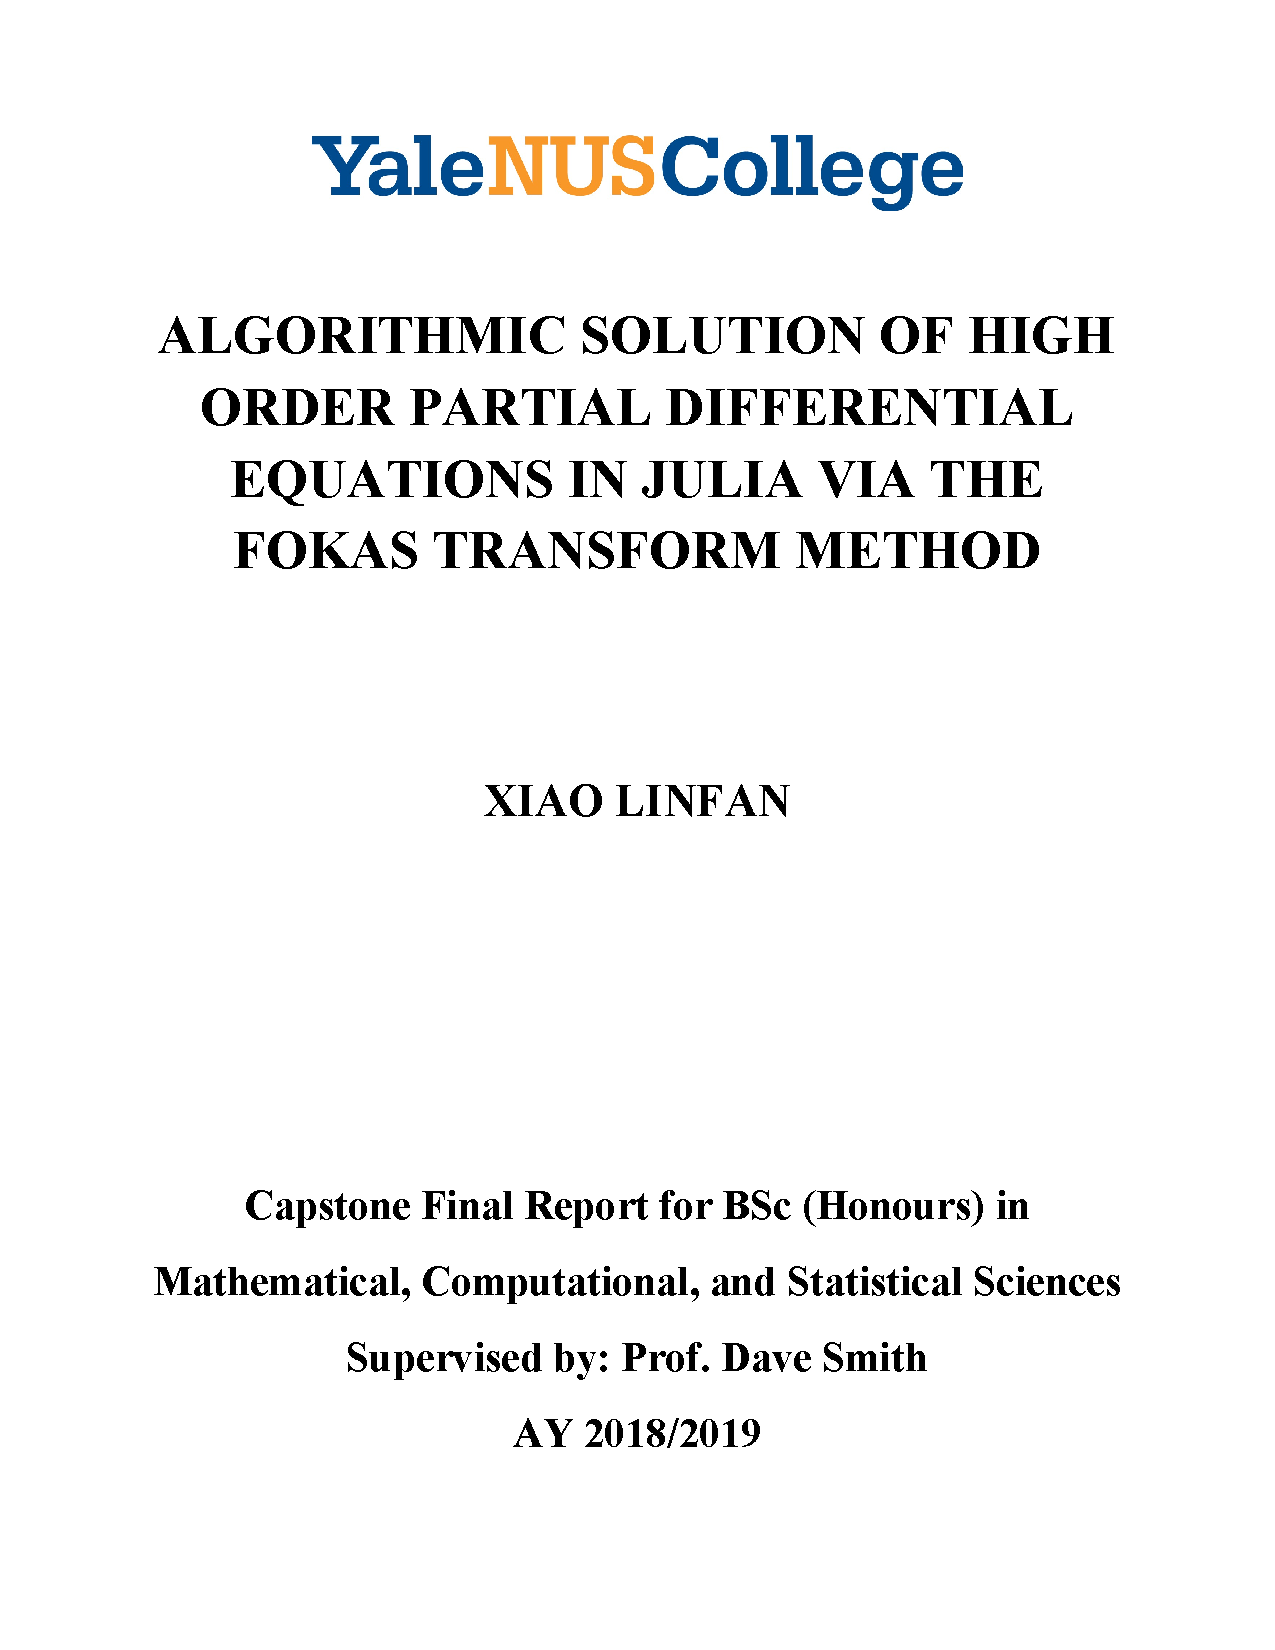
\includepdf[pages={1}]{title_page.pdf}
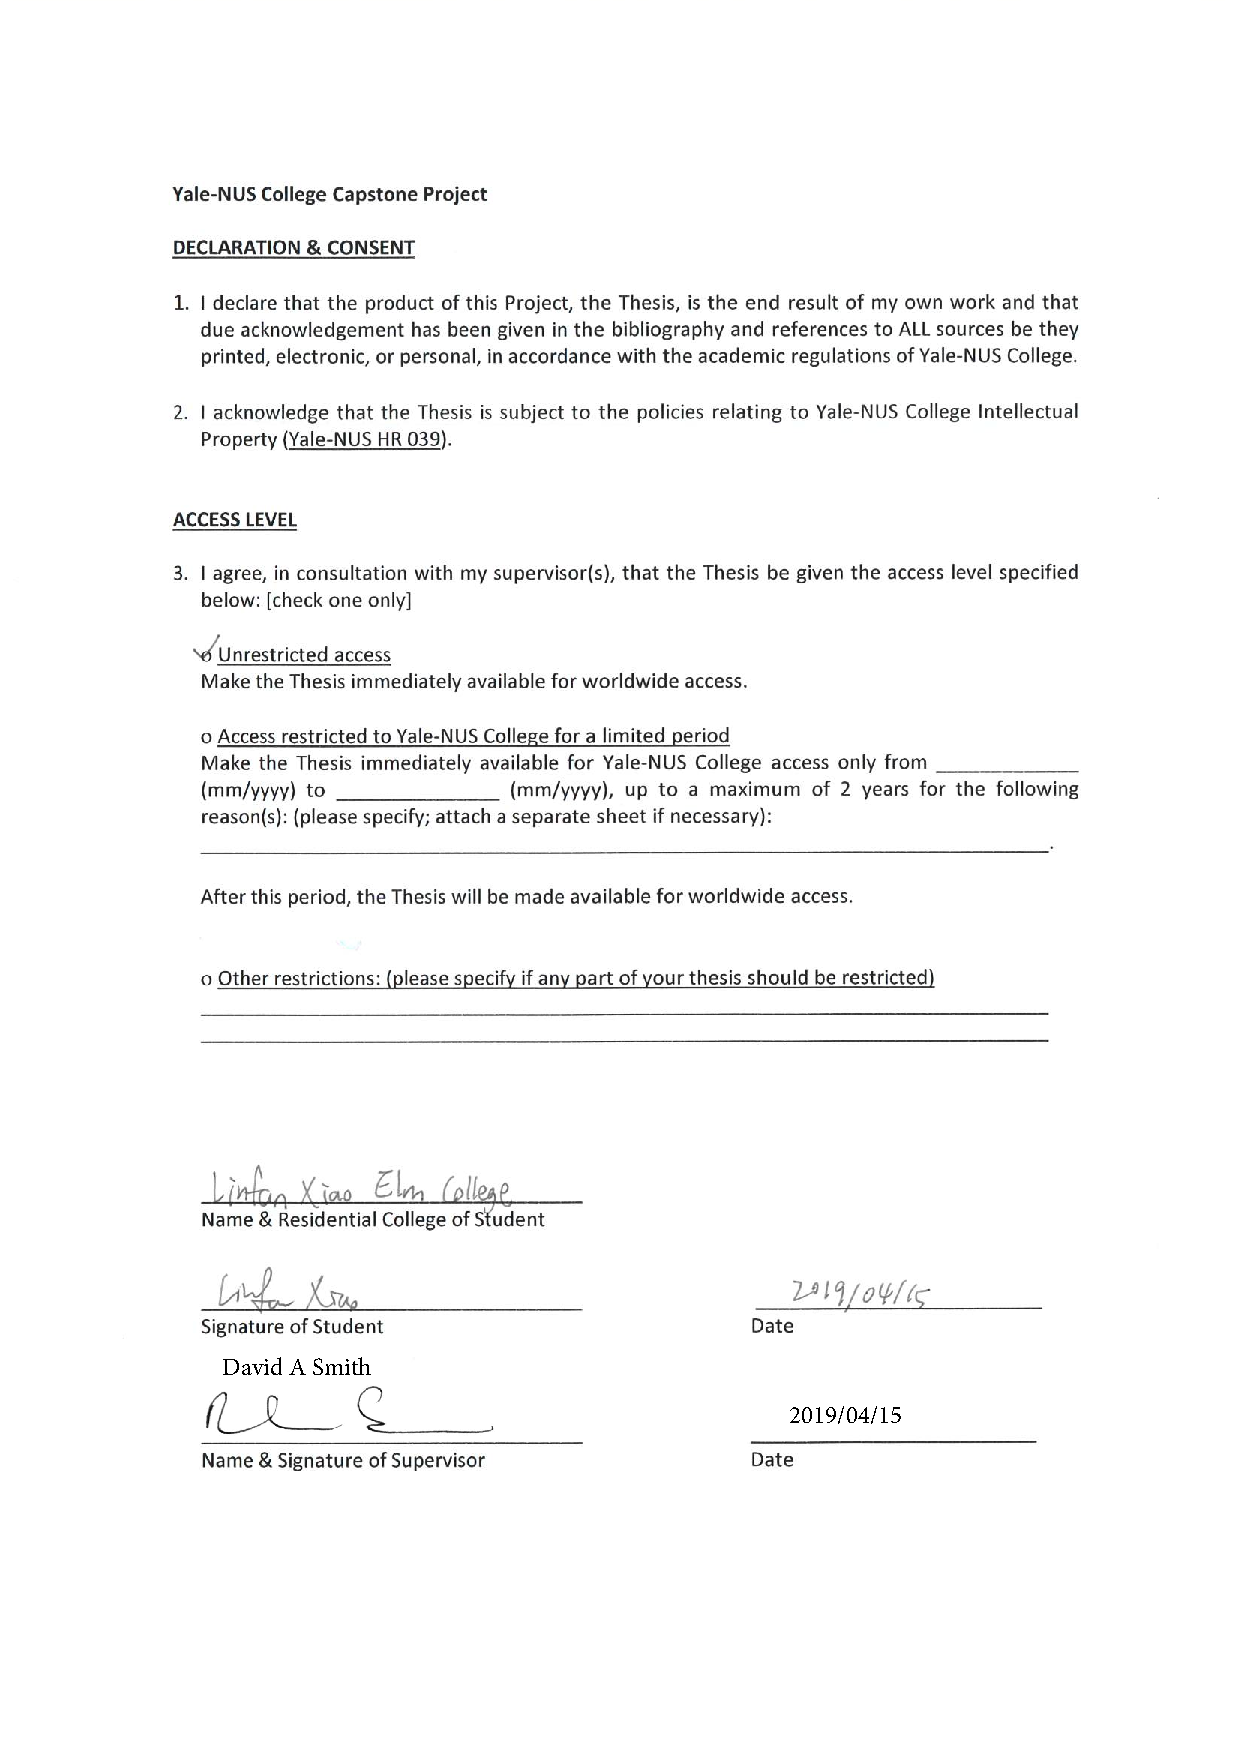
\includepdf[pages={1}]{declaration_form_signed.pdf}
\pagenumbering{gobble}
\tableofcontents
% \listoffigures
% \listoftables
\pagebreak
\pagenumbering{gobble}
% \begin{center}\section*{Acknowledgements}\end{center}
% \addcontentsline{toc}{section}{Acknowledgements}
% I thank Linkin Park, Imagine Dragons, Two Steps from Hell, Paramount Pictures, Marvel Entertainment, and Netflix for providing mental sustenance throughout my capstone project.

\pagebreak
\pagenumbering{arabic}

\section{Introduction}\label{sec:intro}
Evolution partial differential equations (PDEs) relate a quantity to its rates of change with respect to both time and position. Evolution PDEs can model a variety of phenomena, such as heat flow, wave propagation, and particle motion. This project concerns implementing an algorithmic procedure to solve a class of initial-boundary value problems (IBVPs) for linear evolution PDEs of arbitrary spatial order in the finite interval \cite{Smith2016} based on the Fokas transform method \cite{Fokas2000}\cite{Fokas2001}\cite{Fokas2008}\cite{Smith2012}\cite{Deconinck2014}\cite{Fokas2015}. The implementation is developed in Julia \cite{julia}, featuring symbolic computation along with numeric evaluation.

\subsection{Motivation}\label{sec:motivation}
%To motivate the project, suppose we want to solve some IBVPs.

IBVPs arise naturally in the study of physical systems. Certain IBVPs (henceforth referred to as type I problems) can be solved algorithmically via classical transform pairs such as the Fourier transform (Figure \ref{fig:classical_transform}). 
\begin{figure}[htpb!]
    \centering
    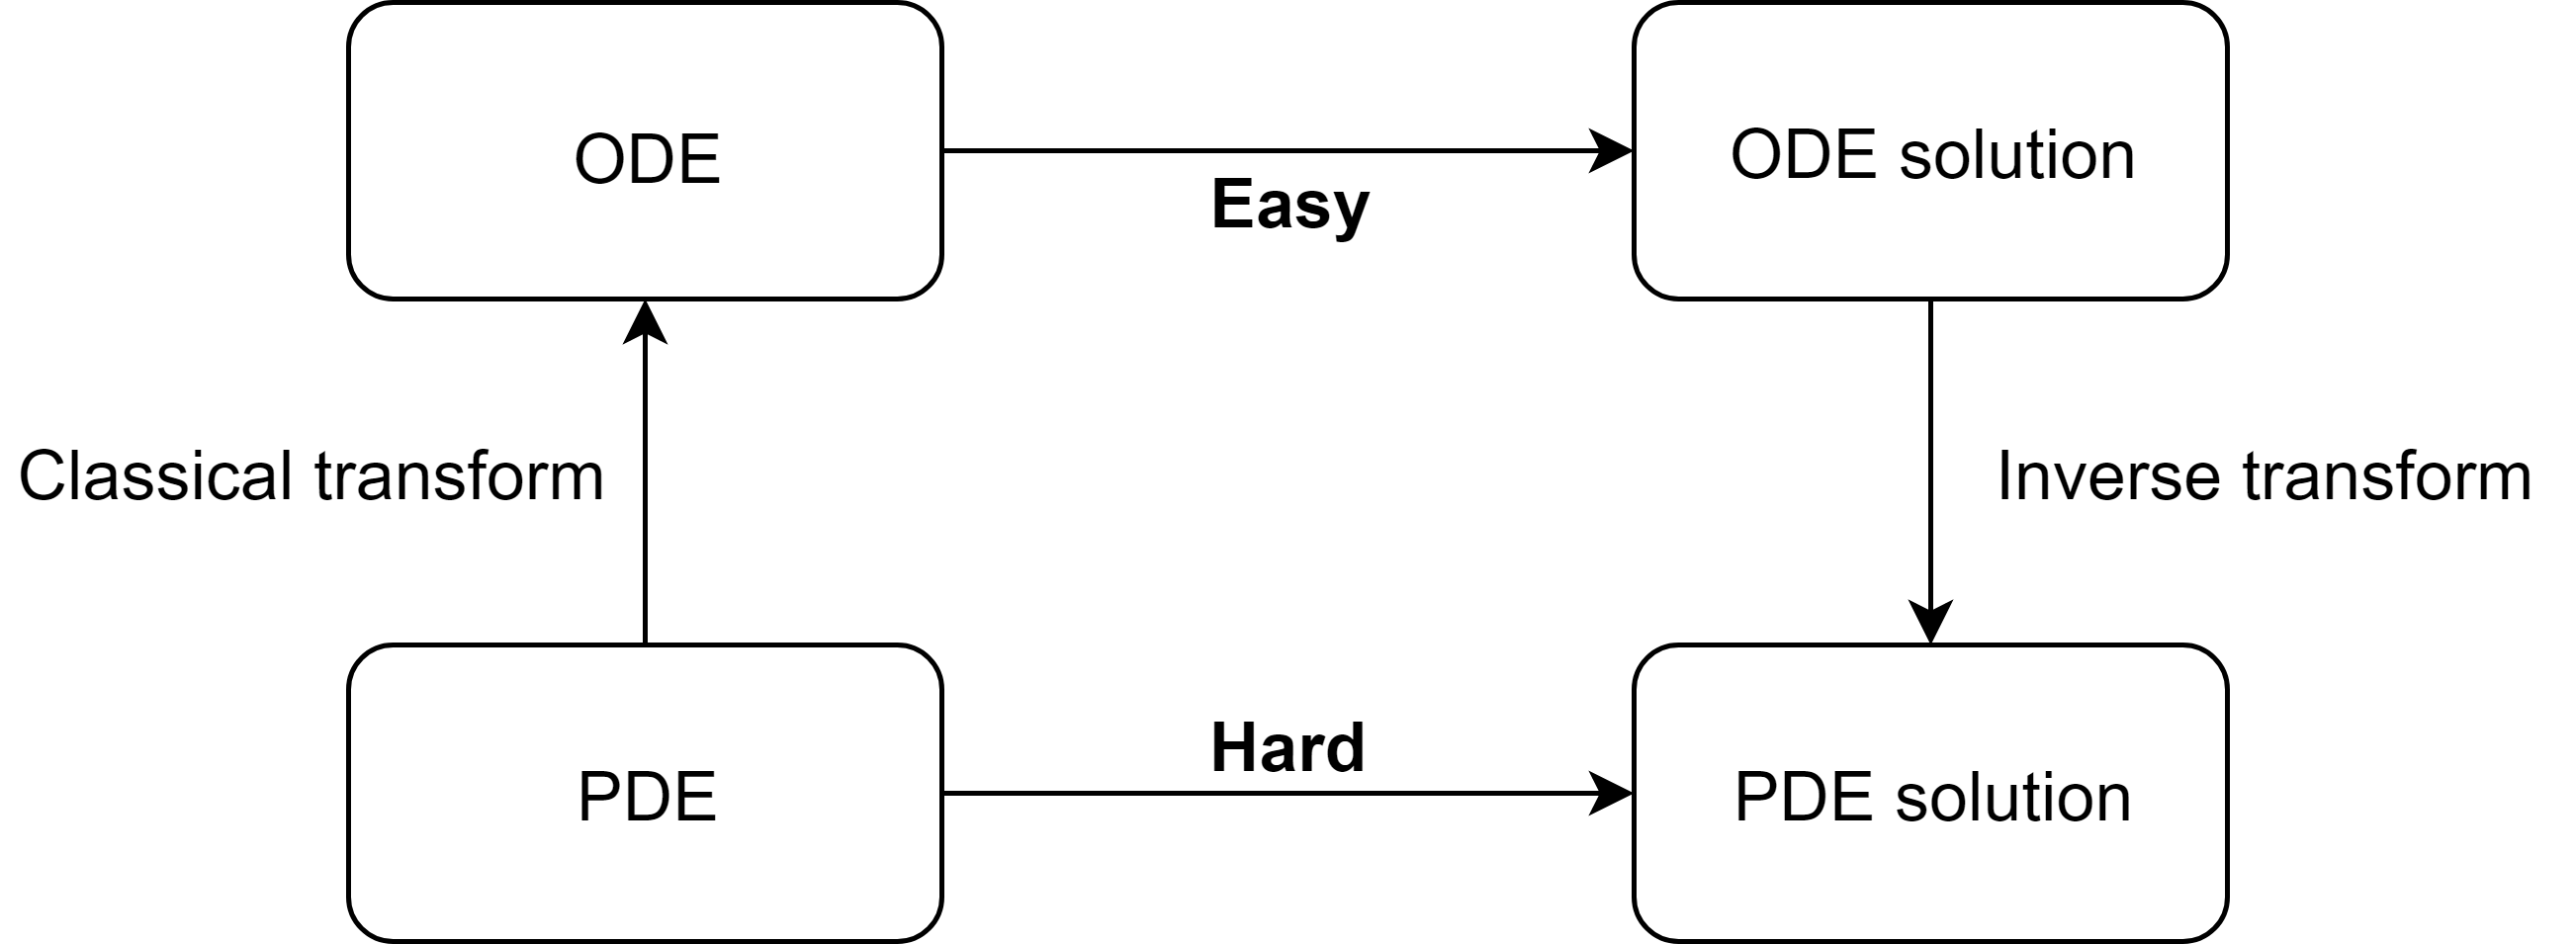
\includegraphics[width=0.8\textwidth]{classical_transform.png}
    \caption{Solving type I IBVPs using classical transform pairs.}
    \label{fig:classical_transform}
\end{figure}

\noindent For example, the heat equation \cite{Pinsky1991}
\[u_t = Ku_{xx},\quad (x,t)\in (0, L)\times (0,\infty)\]
with periodic boundary conditions
\begin{alignat*}{3}
    u(0, t) &= u(L, t),&\quad t&\in (0,\infty)\\
    u_x(0, t) &= u_x(L, t),&\quad t&\in (0,\infty)
\end{alignat*}
and initial datum
\[u(x,0) = f(x), \quad x\in (0, L)\]
can be turned into an ordinary differential equation (ODE) in the temporal variable $t$
\[U_t = -K\lambda^2U\]
with initial datum
\[U(\lambda,0) = F(\lambda),\quad \lambda\in (0,L).\]
where $U(\lambda,t):=\mathcal{F}[u]$ and $F(\lambda):=\mathcal{F}[f]$ are the Fourier transforms of $u(x,t)$ and $f(x)$ with respect to $x$, respectively. This initial-value problem (IVP) for the ODE can be solved directly as 
\[U(\lambda,t) = F(\lambda)e^{-\lambda^2 K t},\]
which, when applying the inverse Fourier transform, gives the IBVP solution $u(x,t)$.

% Similarly, the linear Schr\"{o}dinger equation \cite{Taylor2018} for a free particle given by 
% \[ih w_t(x,t) = -\frac{h^2}{2m}w_{xx}(x,t)\]
% with periodic boundary conditions can be turned into an ODE
% \[W_t(s,t) = \frac{h}{2mi} s^2W(s,t),\]
% where $W(s,t):=\mathcal{F}[w]$ is the Fourier transform of the wave function $w(x,t)$.

For more complicated IBVPs (henceforth referred to as type II problems), no such classical transform pairs exist. The linearized Korteweg-de Vries (linearized KdV) equation which describes shallow water waves \cite{Korteweg1895},
\begin{equation}\label{eq:linearied_kdv}
    u_t + u_{xxx} = 0,
\end{equation}
is one such example. Solving type II problems typically requires a combination of ad-hoc methods, which are often specific to the given problem and cannot be generalized to related problems with different parameters (e.g., IBVPs involving PDEs of different orders or different boundary conditions).

The Fokas transform method extends the idea of classical transform pairs to solving type II problems by constructing non-classical transform pairs (henceforth referred to as the Fokas transform pairs) based on the IBVP parameters. In other words, the Fokas method ``customizes'' appropriate transform pairs for a class of related IBVPs with different parameters; this class of IBVPs can then be solved algorithmically in a manner similar to Figure \ref{fig:classical_transform}, as illustrated in Figure \ref{fig:fokas_transform}.
\begin{figure}[htpb!]
    \centering
    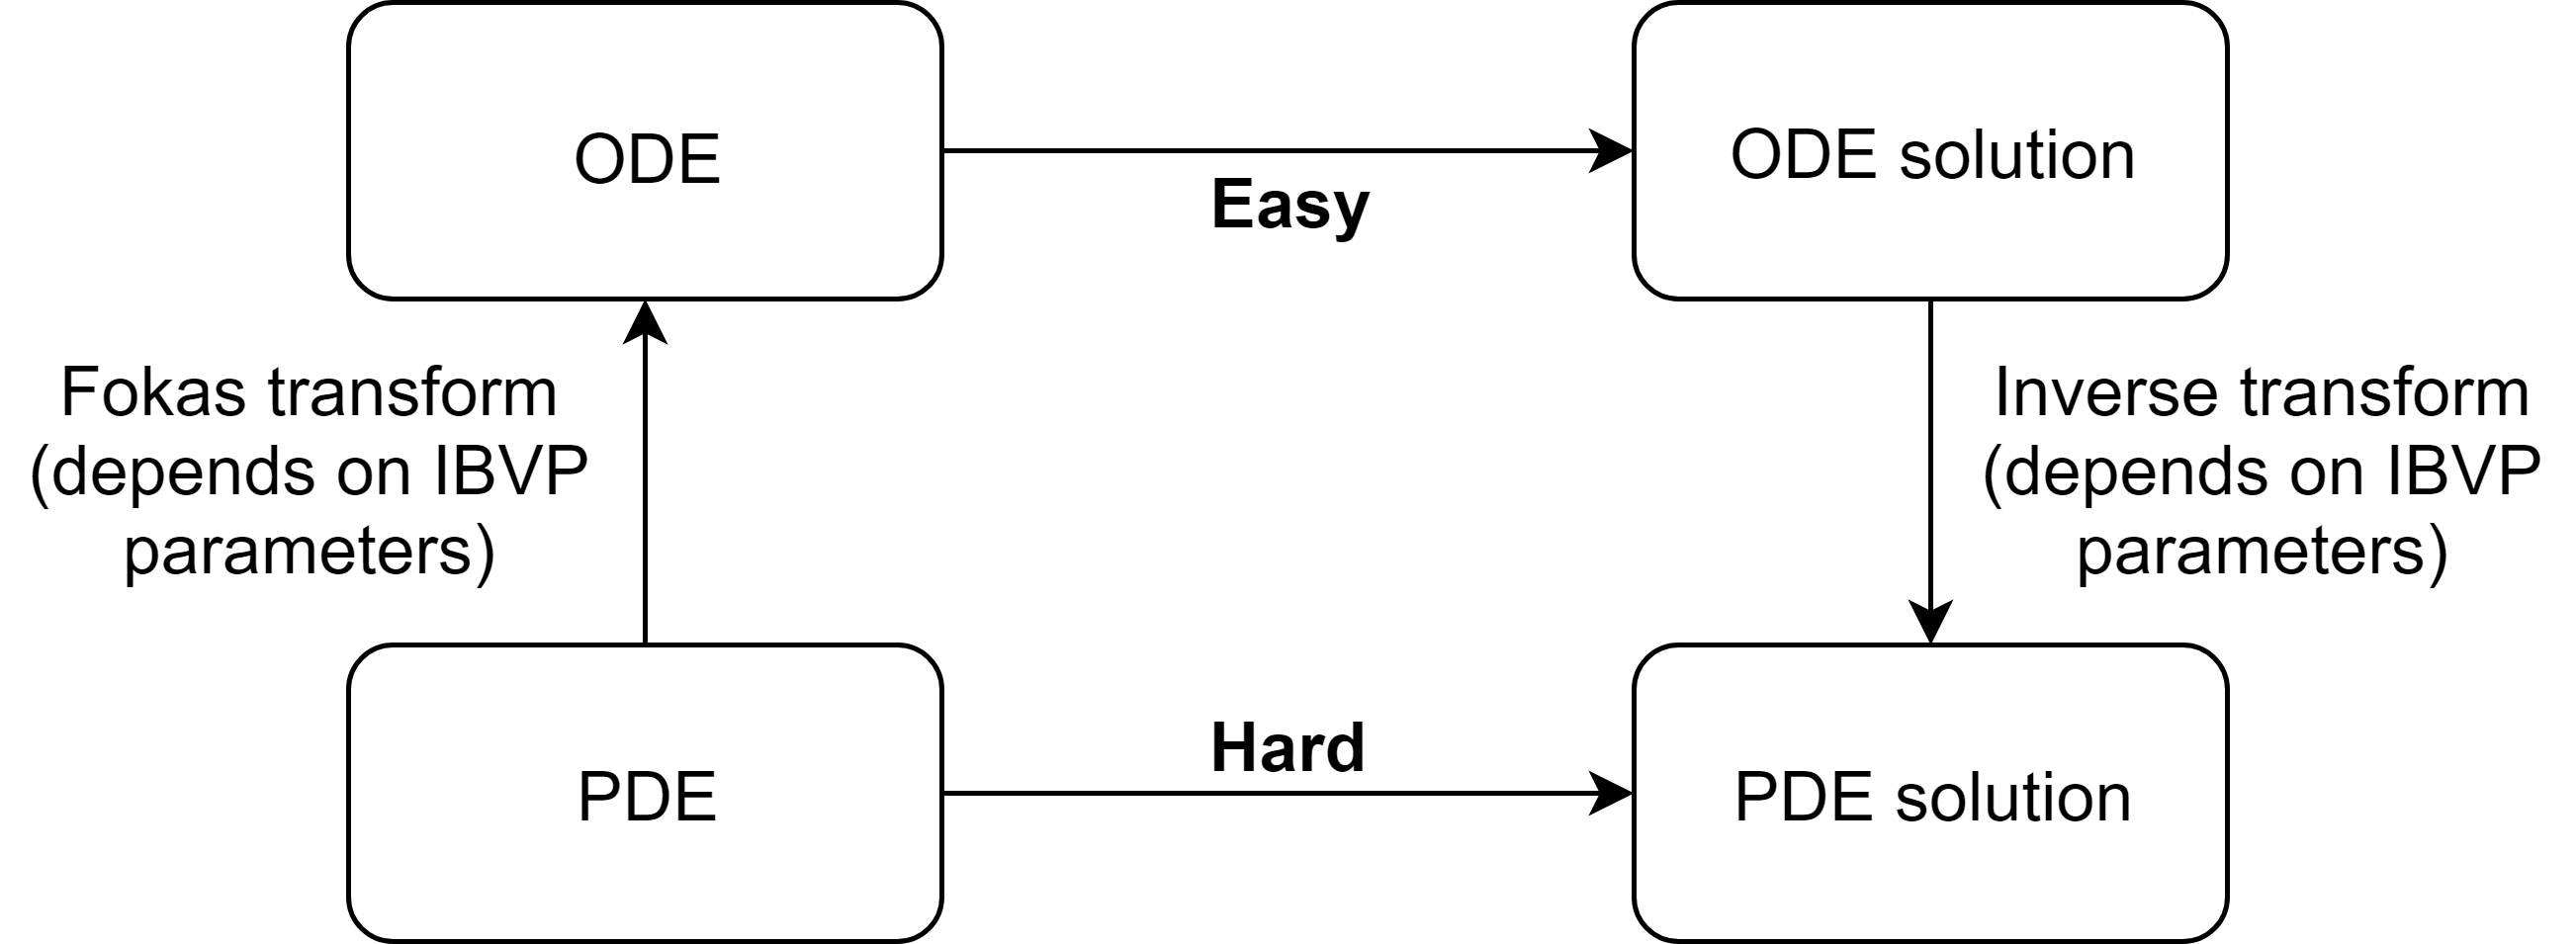
\includegraphics[width=0.8\textwidth]{fokas_transform.png}
    \caption{Solving type II IBVPs using the Fokas transform pairs.}
    \label{fig:fokas_transform}
\end{figure}

A thorough presentation of the Fokas method can be found in \cite{Fokas2008}, and a pedagogical introduction in \cite{Deconinck2014}. Yet the history of the Fokas method can be traced back to a general approach to solving IBVPs for linear and integrable nonlinear PDEs, introduced in 1997 \cite{Fokas1997}. Research efforts thus inspired motivated the discovery of a new transform method to solve boundary-value problems (BVPs) for linear evolution PDEs in two dimensions with arbitrary spatial order (i.e., arbitrary order in the derivative of the spatial variable) in 2000 \cite{Fokas2000}. The Fokas method for two-point BVPs for linear evolution PDEs was proposed in \cite{Fokas2001}. The discussion was expanded to a complete analysis of third and higher-order two-point BVPs in \cite{Smith2012}. Ongoing research is extending the Fokas method to various settings, such as PDEs of fractional order \cite{Fernandez2018}.

This project focuses on the Fokas method for IBVPs \cite{Smith2016}. Examples of IBVPs that can be solved by the Fokas method include the following IBVPs for the linearized KdV equation \cite{Smith2016}:
\begin{subequations}\label{eq:problem_1}
    \begin{alignat}{3}
        q_t(x,t) + q_{xxx}(x,t) &= 0,\quad &(x,t)&\in (0,1)\times (0,T)\\
        q(x,0) &= f(x),\quad &x&\in [0,1]\\
        q(0,t) = q(1,t) &= 0, \quad &t&\in [0,T]\\
        q_x(1,t) &= \frac{1}{2}q_x(0,t)\quad &t&\in [0,T],
    \end{alignat}
\end{subequations}
and 
\begin{subequations}\label{eq:problem_2}
    \begin{alignat}{3}
        q_t(x,t) + q_{xxx}(x,t) &= 0,\quad &(x,t)&\in (0,1)\times (0,T)\\
        q(x,0) &= f(x),\quad &x&\in [0,1]\\
        q(0,t) = q(1,t) = q_x(1,t) &= 0, \quad &t&\in [0,T].
    \end{alignat}
\end{subequations}
% \[q_t(x,t) + a(-i)^2 q_{xx}(x,t) = 0,\]
% with boundary conditions
% \begin{equation}\label{eq:informal_example}
%     \begin{split}
%     q(0,t) + c_0q(1,t) &= 0\\
%     q_x(0,t) + c_1q_x(1,t) &= 0,
%     \end{split}
% \end{equation}
% or
% \begin{align*}
%     q(0,t) + c_0 q_x(0,t) &= 0\\
%     q(1) + c_1 q_x(1,t) &= 0,
% \end{align*}
% where $c_0, c_1\in\widehat{\C}:=\C\cup\{0,\infty\}$ (in the sense that if $c_0=\infty$ in equation \eqref{eq:informal_example}, then dividing by $c_0$ makes $q(0,t)$ disappear and leaves the first equation as $q(1,t) = 0$), as well as third order PDEs of the form 
% \[q_t(x,t) \pm i(-i)^2 q_{xxx}(x,t) = 0,\]
% with boundary conditions
% \begin{align*}
%     q(0,t) + c_0 q(1,t) &= 0\\
%     q_x(0,t) + c_1 q_x(1,t) &= 0\\
%     q_{xx}(0,t) + c_2 q_{xx}(1,t) &= 0,
% \end{align*}
% where $c_j\in\widehat{\C}$ for $j=0,1,2$, or 
% \begin{align*}
%     q(0,t) &= 0\\
%     q(1,t) &= 0\\
%     q_x(0,t) + c q_x(1,t) &= 0,
% \end{align*}
% where $c\in\widehat{\C}$. 

As mentioned earlier and will be shown later, beyond the two examples above, the Fokas method is in fact applicable to IBVPs with arbitrary spatial order. PDEs of higher order are generally not as well understood as their first and second order counterparts. The Fokas method thus advances the understanding of higher order PDEs by providing an algorithmic procedure to solve an entire class of IBVPs of arbitrary spatial order. Applying the Fokas method by hand, however, is laborious. It is thus of interest to implement the Fokas method as a software library that aims to supply as much computer aid as possible in the computation process. The types of computer aid include visualizations of integration contours, numeric evaluation, and more importantly, derivation of explicit symbolic formulas for important mathematical objects which would help proving technical lemmas that arise in applying the Fokas method to IBVPs \cite{Smith2012} and beyond \cite{Miller2018}.

In this project, the implementation of the Fokas method is developed in Julia, a free open-source, high-performance language for numerical computing \cite{julia}. Among tools for numerical computing, commercial software packages may provide functionalities to execute sophisticated computational tasks; yet due to being closed-source, there exists a lack of transparency which limits users' understanding of the nature of the software output. As a result, there has been a trend in the mathematical community that encourages the use of open-source languages like Julia, which allows users to verify the correctness of the output. Therefore, we choose Julia to be the language of implementation. At the start of this project, the latest release of Julia is 1.0; however, existing graphical libraries in Julia were not yet made compatible with Julia 1.0 at that time. Thus, this project uses the next latest release of Julia that is stable at that time, namely Julia 0.6.4. 

To the best of our knowledge, despite the presence of various differential equation solvers in mathematical software such as Julia, Mathematica, and Matlab, this is the first time that the Fokas method is implemented computationally in any generality, and it allows solving a particular class of IBVPs for which no other general analytic solver algorithm yet exists.

\subsection{The initial-boundary value problem}\label{sec:IBVP}
To formally characterize the class of IBVPs that can be solved by the Fokas method \cite[p.9]{Smith2016}, we first introduce the following definitions.

Define linearly independent boundary forms $B_j: C^\infty[0,1]\to \C$ (where $C^\infty[0,1]$ denotes the class of real-valued functions differentiable for all orders on $[0,1]$) by
\begin{equation}\label{eq:B_j}
    B_j\phi := \sum_{k=0}^{n-1}\left(b_{jk}\phi^{(k)}(0) + \beta_{jk}\phi^{(k)}(1)\right),\, j\in\{1,2,\ldots,n\}
\end{equation}
where the boundary coefficients $b_{jk}$, $\beta_{jk}\in\R$. 

Define the set of smooth functions $\phi$ that satisfy the homogeneous boundary conditions $B_j\phi=0$ for $j\in\{1,2,\ldots,n\}$ as
\begin{equation}\label{eq:Phi}
    \Phi:=\{\phi\in C^\infty[0,1]:\, B_j\phi = 0\,\forall j\in\{1,2,\ldots,n\}\}.
\end{equation}

Define a spatial differential operator (i.e., a differential operator in the spatial variable $x$) of order $n$ to be
\begin{equation}\label{eq:S}
    S := (-i)^n \frac{d^n}{dx^n}.
\end{equation}

The Fokas method allows solving any well-posed IBVP that can be written in the form
\begin{subequations}\label{eq:IBVP}
    \begin{alignat}{3}
        (\partial_t + aS)q(x,t) &= 0\quad &\forall (x,t)&\in (0,1)\times (0,T) \label{eq:PDE}\\
        q(x,0) &= f(x)\in \Phi\quad &\forall x&\in [0,1]\label{eq:initial_condition}\\
        q(\cdot, t) &\in \Phi \quad &\forall t&\in [0,T],\label{eq:boundary_condition}
    \end{alignat}
\end{subequations}
where $a$ is a complex constant. For the IBVP to be well-posed, we require at least that $a=\pm i$ if $n$ is odd and $\real(a)\geq 0$ if $n$ is even. Equation \eqref{eq:PDE} is a PDE in the spatial variable $x$ and the temporal variable $t$ with arbitrary spatial order $n$.
%relating a quantity $q$ to its temporal and spatial rates of change $\partial_t[q]$ and $aS[q]$. 
Equation \eqref{eq:initial_condition} is an initial datum where the temporal variable $t=0$. Equation \eqref{eq:boundary_condition} corresponds to the homogeneous spatial boundary conditions, specifying that for any fixed $t\in [0,T]$, $q(x,t)=:\phi(x)$ as a function of $x$ satisfies $B_j\phi=0$ for $j\in \{1,2,\ldots,n\}$.

The linearized KdV equations introduced in equation \eqref{eq:linearied_kdv} are examples of such IBVPs. Specifically, IBVP \eqref{eq:problem_1} can be written in the form of \eqref{eq:IBVP} with $a=-i$,
\[S = (-i)^3 \frac{d^3}{dx^3} = i\frac{d^3}{dx^3},\]
\begin{align*}
    B_1 \phi &= 1\cdot\phi(0) + 0\cdot\phi(1) + 0\cdot\phi^{(1)}(0) + 0\cdot\phi^{(1)}(1) + 0\cdot\phi^{(2)}(0) + 0\cdot\phi^{(2)}(1)\\
    B_2 \phi &= 0\cdot\phi(0) + 1\cdot\phi(1) + 0\cdot\phi^{(1)}(0) + 0\cdot\phi^{(1)}(1) + 0\cdot\phi^{(2)}(0) + 0\cdot\phi^{(2)}(1)\\
    B_3 \phi &= 0\cdot\phi(0) + 0\cdot\phi(1) + 1\cdot\phi^{(1)}(0) - 2\cdot\phi^{(1)}(1) + 0\cdot\phi^{(2)}(0) + 0\cdot\phi^{(2)}(1),
\end{align*}
and 
\[\Phi = \{\phi\in C^{\infty}[0,1]:\, B_j\phi = 0\,\forall j\in\{1,2,3\}\}.\]
Similarly, IBVP \eqref{eq:problem_2} can be written in the form of \eqref{eq:IBVP} with $a=-i$,
\[S = (-i)^3 \frac{d^3}{dx^3} = i\frac{d^3}{dx^3},\]
\begin{align*}
    B_1 \phi &= 1\cdot\phi(0) + 0\cdot\phi(1) + 0\cdot\phi^{(1)}(0) + 0\cdot\phi^{(1)}(1) + 0\cdot\phi^{(2)}(0) + 0\cdot\phi^{(2)}(1)\\
    B_2 \phi &= 0\cdot\phi(0) + 1\cdot\phi(1) + 0\cdot\phi^{(1)}(0) + 0\cdot\phi^{(1)}(1) + 0\cdot\phi^{(2)}(0) + 0\cdot\phi^{(2)}(1)\\
    B_3 \phi &= 0\cdot\phi(0) + 0\cdot\phi(1) + 0\cdot\phi^{(1)}(0) + 1\cdot\phi^{(1)}(1) + 0\cdot\phi^{(2)}(0) + 0\cdot\phi^{(2)}(1),
\end{align*}
and 
\[\Phi = \{\phi\in C^{\infty}[0,1]:\, B_j\phi = 0\,\forall j\in\{1,2,3\}\}.\]

% An example of such IBVPs is the linear Schr\"{o}dinger equation \cite{Taylor2018}, which describes the wave form of a quantum system in free space. The linear Schr\"{o}dinger equation with zero potential is given by
% \[ih\frac{\partial}{\partial t}w + \frac{h^2}{2m}\frac{\partial^2}{\partial x^2}w = 0,\]
% where $w(x,t)$ is the wave function, $h$ is the Planck's constant, $m$ is the mass of the particle, and $kx$ describes the potential energy of the particle in the force field. It can be written in the form of \eqref{eq:PDE} as
% \[(\partial_t + aS)q(x,t) = 0\]
% where $q=w$, $S = \frac{\partial^2}{\partial x^2}$, and $a = \frac{h}{2mi}$. The initial datum 
% \[w(x,0) = w_0(x)\]
% would mean that the system's wave form at initial stage is described by the wave function $w_0(x)$, and the boundary conditions 
% \[w(\cdot, t) = f\]
% would mean that the behaviour of the system at its boundary is described by the function $f$ (e.g., if we are considering particles moving in a box, $f$ would describe how the particles behave at the box's boundaries).

For appropriate transform $F_\lambda$ and inverse transform $f_x$ pair found using the Fokas method (to be explained in detail later), the solution to the IBVP characterized above is given by \cite[p.15]{Smith2016}
\begin{equation}\label{eq:q(x,t)}
    q(x,t) = f_x(e^{-a\lambda^n t}F_\lambda(f)),
\end{equation}
thus completing the procedure summarised in Figure \ref{fig:fokas_transform}.

\section{Preliminaries}
We now begin to introduce the preliminary definitions and results used in the algorithmic procedure that finds \eqref{eq:q(x,t)}. The key to the algorithm is the construction of the Fokas transform pair, which in turn depends on finding a valid adjoint of the given boundary conditions. Thus, we devote the following sections to characterizing the adjoint, and by doing so, outline its construction. This section presents material from chapter 11 of \cite{CoddingtonLevinson}, with proofs expanded and completed, and the utility of the theorems expounded.

\subsection{Homogeneous boundary value problems}
\begin{defn}\cite[p.81]{CoddingtonLevinson}\label{defn:linear differential operator}
    A \textbf{linear differential operator} $L$ of order $n$ ($n>1$) on interval $[a,b]$ is defined by
    \begin{equation}\label{eq:L}
        Lx = p_0x^{(n)} + p_1x^{(n-1)} + \cdots + p_{n-1}x' + p_nx,
    \end{equation}
    where the $p_k$ are complex-valued functions of class $C^{n-k}$ on $[a,b]$ and $p_0(t)\neq 0$ on $[a,b]$.
\end{defn}

\begin{defn}\cite[p.284]{CoddingtonLevinson}\label{defn:homogeneous boundary conditions}
    \textbf{Homogeneous boundary conditions} refer to a set of equations of the type
    \begin{equation}\label{eq:homogeneous boundary conditions}
        \sum_{k=1}^n (M_{jk}x^{(k-1)}(a) + N_{jk}x^{(k-1)}(b))=0 \quad (j=1,\ldots,m) 
    \end{equation}
    where $M_{jk}, N_{jk}$ are complex constants.
\end{defn}

\begin{defn}\cite[p.284]{CoddingtonLevinson}\label{defn:homogeneous boundary value problem}
    A \textbf{homogeneous boundary value problem} concerns finding the solutions of 
    \[Lx=0\] on some interval $[a,b]$ which satisfy some homogeneous boundary conditions.
\end{defn}

\subsection{Adjoints of homogeneous boundary value problems}\label{sec:adjoints_of_homogeneous_BVPs}

Recall from linear algebra that, given a linear map $T$ from inner product spaces $V$ to $W$, the adjoint of $T$ is the function $T^\star:W\to V$ with
\begin{equation}\label{eq:linear map adjoint}
    \langle Tv, w\rangle = \langle v, T^\star w\rangle
\end{equation}
for $v\in V$, $w\in W$, where $\langle \cdot,\,\cdot \rangle$ denotes the inner product defined on $V$ and $W$ \cite[p.204]{Axler1997}. There exists a similar notion for boundary value problems, which we begin to formulate below.

\subsubsection{Adjoint differential operator}
\begin{defn}\cite[p.84]{CoddingtonLevinson}\label{defn:adjoint linear differential operator}
    Given a linear differential operator $L$ of order $n$ as in Definition \ref{defn:linear differential operator}, the operator $L^+$ given by
    \[L^+x = (-1)^n (\bar{p}_0 x)^{(n)} + (-1)^{n-1}(\bar{p}_1 x)^{(n-1)} +\cdots +\bar{p}_nx\]
    (where $\bar{p}_k$ denotes the complex conjugate of $p_k$ for $k\in\{0,\ldots,n\}$) is the \textbf{adjoint} of $L$.
\end{defn}

\subsubsection{Adjoint boundary conditions}
For a homogeneous boundary value problem $\pi$ with linear differential operator $L$ and some homogeneous boundary conditions, an adjoint problem $\pi^+$ involves the adjoint linear differential operator $L^+$ and a set of homogeneous adjoint boundary conditions. The adjoint boundary conditions are such that an equation similar to \eqref{eq:linear map adjoint} holds for solutions of $\pi$ and those of $\pi^+$, with the inner product $\langle\cdot,\,\cdot\rangle$ defined as $\langle u,v\rangle := \int_a^b u\bar{v}\,dt$ for $u, v\in C^n$ on $[a,b]$. In the following sections, we seek to characterize the adjoint boundary conditions and their construction.

The construction depends on two important results, namely Green's formula and the boundary-form formula. Green's formula allows characterizing a form, which, when used in the boundary-form formula, gives rise to the desired construction. 

We begin with Green's formula.

\paragraph{Green's formula}
\begin{thm}\cite[p.284]{CoddingtonLevinson}{(Green's formula)}\label{thm:green's formula}
    For $u, v\in C^n$ on $[a,b]$,
    \begin{equation}\label{eq:green's formula}
        \int_{t_1}^{t_2}(Lu)\bar{v}\,dt - \int_{t_1}^{t_2}u(\overline{L^+v})\,dt = [uv](t_2) - [uv](t_1) 
    \end{equation}
    where $a\leq t_1<t_2\leq b$ and $[uv](t)$ is the form in $(u, u', \ldots, u^{(n-1)})$ and $(v, v', \ldots, v^{(n-1)})$ given by
    \begin{equation}\label{eq:[uv](t) defn}
        [uv](t)=\sum_{m=1}^n\sum_{j+k=m-1}(-1)^j u^{(k)}(t)(p_{n-m}\bar{v})^{(j)}(t)
    \end{equation}
\end{thm}
Using the form $[uv](t)$, we define an important $n\times n$ matrix $B$ whose entries $B_{jk}$ satisfy
\begin{equation}\label{eq:[uv](t) in B matrix}
    \begin{split}
        [uv](t) = \sum_{j,k=1}^n B_{jk}(t)u^{(k-1)}(t)\bar{v}^{(j-1)}(t).
    \end{split}
\end{equation}
Note that
\begin{align*}
    [uv](t) &= \sum_{m=1}^n\sum_{j+k=m-1}(-1)^j u^{(k)}(t)(p_{n-m}\bar{v})^{(j)}(t)\\
        &= \sum_{m=1}^n\sum_{j+k=m-1}(-1)^j u^{(k)}(t)\left(\sum_{\ell=0}^j\binom{j}{\ell}p_{n-m}^{(j-\ell)}(t)\bar{v}^{(\ell)}(t)\right)\\
        &= \sum_{m=1}^n\sum_{k=0}^{m-1}(-1)^{m-1-k} u^{(k)}(t)\left(\sum_{\ell=0}^{m-1-k}\binom{m-1-k}{\ell}p_{n-m}^{(m-1-k-\ell)}(t)\bar{v}^{(\ell)}(t)\right)\\
        &= \sum_{m=1}^n\sum_{k=1}^{m}(-1)^{m-k}\left(\sum_{\ell=0}^{m-k}\binom{m-k}{\ell}p_{n-m}^{(m-k-\ell)}(t)\bar{v}^{(\ell)}(t)\right)u^{(k-1)}(t)\quad\mbox{(shifting $k$ to $k+1$)}\\
        &= \sum_{k=1}^n\sum_{m=k}^n (-1)^{m-k}\left(\sum_{\ell=0}^{m-k}\binom{m-k}{\ell}p_{n-m}^{(m-k-\ell)}(t)\bar{v}^{(\ell)}(t)\right)u^{(k-1)}(t).
\end{align*}

To find $B_{jk}$, we need to extract the coefficients of $u^{(k-1)}\bar{v}^{(j-1)}$. We first note that, fixing $m$ and $k$, when $\ell=j-1$, the coefficient of $\bar{v}^{(j-1)}$ is
\begin{align*}
    \binom{m-k}{j-1}p_{n-m}^{(m-k-j+1)}(t).
\end{align*}
To find the coefficient of $u^{(k-1)}\bar{v}^{(j-1)}$, we need to fix $k$ and collect the above coefficient across all values of $m$. Since $m$ goes up to $n$, $m-k$ goes up to $n-k$. Since $\ell\leq m-k$, $\ell=j-1$ implies $j-1\leq m-k$. Thus, $m-k$ ranges from $j-1$ to $n-k$. Let $\ell':=m-k$, then $m=k+\ell'$, and the above equation becomes
\begin{align*}
    [uv](t) 
    &= \sum_{k=1}^n\sum_{j=1}^n (-1)^{\ell'}\left(\sum_{\ell'=j-1}^{n-k}\binom{\ell'}{j-1}p_{n-(k+\ell')}^{(\ell'-(j-1))}(t)\right)\bar{v}^{(j-1)}(t)u^{(k-1)}(t)\\
    &= \sum_{j,k=1}^n \left(\sum_{\ell=j-1}^{n-k}\binom{\ell}{j-1}p^{(\ell-j+1)}_{n-k-\ell}(t)(-1)^\ell\right)u^{(k-1)}(t)\bar{v}^{(j-1)}(t)\quad\mbox{(replace $\ell'$ by $\ell$)}.
\end{align*}
Thus,
\[B_{jk}(t) = \sum_{\ell=j-1}^{n-k}\binom{\ell}{j-1}p^{(\ell-j+1)}_{n-k-\ell}(t)(-1)^\ell.\]
We note that for $j+k>n+1$, or $j-1>n-k$, $\ell$ is undefined, for the terms $u^{(k-1)}(t)\bar{v}^{(j-1)}(t)$ with $j+k>n+1$ do not exist in $[uv](t)$. Thus, $B_{jk}(t)=0$. Also, for $j+k=n+1$, or $j-1=n-k$,
\[B_{jk}(t) = \binom{j-1}{j-1}p^{(j-1-j+1)}_{j-1-(j-1)}(t)(-1)^{j-1} = (-1)^{j-1}p_0(t).\] 
Thus, the matrix $B$ has the form
\begin{equation}\label{eq:B(t)}
    B(t)=\begin{bmatrix}
        B_{11} & B_{12} & \cdots & \cdots & B_{1\,n-1} & p_0(t)\\
        B_{21} & B_{22} & \cdots & \cdots & -p_0(t) & 0\\
        \vdots & \vdots & \ddots &  & \vdots & \vdots\\
        \vdots & \vdots &  & \ddots & \vdots & \vdots\\
        (-1)^{n-1}p_0(t) & 0 & \cdots & \cdots & 0 & 0
    \end{bmatrix}.
\end{equation}
We note that because $p_0(t)\neq 0$ on $[a,b]$ (as required in Definition \ref{defn:linear differential operator}), $B(t)$ is square with $\det B(t)=(p_0(t))^n\neq 0$ on $[a,b]$. Thus, $B(t)$ is nonsingular for $t\in [a,b]$.


Now we seek another matrix $\widehat{B}$ that embodies both the characteristics of $B$ and those of the interval $[a,b]$. This concerns writing the right-hand side of Green's formula in matrix form. We begin by introducing the following definitions.

\begin{defn}\cite[p.285]{CoddingtonLevinson}\label{defn:f cdot g}
    For vectors $f=(f_1,\ldots,f_k)$ and $g=(g_1,\ldots,g_k)$, define the product
    \[f\cdot g:=\sum_{i=1}^k f_i\bar{g}_i.\]
    Note that $f\cdot g = g^*\cdot f$ where $^*$ denotes the conjugate transpose.
\end{defn}

\begin{defn}\cite[p.285]{CoddingtonLevinson}\label{defn:semibilinear form}
    A \textbf{semibilinear form} is a complex-valued function $\mathcal{S}$ defined for pairs of vectors $f=(f_1,\ldots,f_k)$, $g=(g_1,\ldots,g_k)$ satisfying
    \begin{align*}
        \mathcal{S}(\alpha f+\beta g, h)&=\alpha\mathcal{S}(f,h) + \beta\mathcal{S}(g,h)\\
        \mathcal{S}(f, \alpha g + \beta h) &= \bar{\alpha}\mathcal{S}(f,g) + \bar{\beta}\mathcal{S}(f, h)
    \end{align*}
    for any complex numbers $\alpha, \beta$ and vectors $f,g,h$.
\end{defn}
We note that if
\[S = \begin{bmatrix}
    s_{11} & \cdots & s_{1k}\\
    \vdots & \ddots & \vdots\\
    s_{k1} & \cdots & s_{kk}
\end{bmatrix},\]
then $Sf\cdot g$ is given by
\begin{equation}\label{eq:semibilinear form}
    \begin{split}
    \mathcal{S}(f,g) &:= Sf\cdot g = \begin{bmatrix}
        s_{11} & \cdots & s_{1k}\\
        \vdots & \ddots & \vdots\\
        s_{k1} & \cdots & s_{kk}
    \end{bmatrix} \begin{bmatrix}
        f_1\\
        \vdots\\
        f_k
    \end{bmatrix} \cdot \begin{bmatrix}
        g_1\\
        \vdots\\
        g_k
    \end{bmatrix} = \begin{bmatrix}
        \sum_{j=1}^k s_{1j}f_j\\
        \vdots\\
        \sum_{j=1}^k s_{kj}f_j
    \end{bmatrix}\cdot \begin{bmatrix}
        g_1\\
        \vdots\\
        g_k
    \end{bmatrix}\\
    &= \sum_{i=1}^k\left(\sum_{j=1}^k s_{ij}f_j\right)\bar{g}_i =\sum_{i,j=1}^k s_{ij}f_i\bar{g}_i.
    \end{split}
\end{equation}
To see that this is a semibilinear form:
\begin{align*}
    \mathcal{S}(\alpha f+\beta g, h)
    &= \sum_{i,j=1}^k s_{ij}(\alpha f_j + \beta g_j)\bar{h}_i
    = \alpha \sum_{i,j=1}^k s_{ij}f_j\bar{h}_i + \beta \sum_{i,j=1}^k g_j\bar{h}_i\\
    &= \alpha Sf\cdot h + \beta Sg\cdot h
    = \alpha\mathcal{S}(f,h) + \beta\mathcal{S}(g,h);
\end{align*}
and similarly,
\begin{align*}
    \mathcal{S}(f, \alpha g + \beta h)
    &= \sum_{i,j=1}^k s_{ij}f_j(\overline{\alpha g_i + \beta h_i})
    = \bar{\alpha}\sum_{i,j=1}^k s_{ij}f_j\bar{g}_i + \bar{\beta}\sum_{i,j=1}^k f_j \bar{h}_i\\
    &= \bar{\alpha}Sf\cdot g + \bar{\beta}Sf\cdot h
    = \bar{\alpha}\mathcal{S}(f,g) + \bar{\beta}\mathcal{S}(f,h).
\end{align*}

Under a similar matrix framework, we see that $[uv](t)$ is a semibilinear form with matrix $B(t)$: Let $\vec{u}=(u, u', \ldots, u^{(n-1)})$ and $\vec{v}=(v, v', \ldots, v^{(n-1)})$. Then we have
\begin{equation}\label{[uv](t) in semibilinear form}
    \begin{split}
    [uv](t) &= \sum_{j,k=1}^n B_{jk}(t)u^{(k-1)}(t)\bar{v}^{(j-1)}(t)\quad\mbox{(by equation \eqref{eq:[uv](t) in B matrix})}\\
    &= \sum_{i,j=1}^n (B_{ij}u^{(j-1)}\overline{v}^{(i-1)})(t)\\
    &= (B\vec{u}\cdot \vec{v})(t)\quad\mbox{(by equation \eqref{eq:semibilinear form})}\\
    &=: \mathcal{S}(\vec{u},\vec{v})(t).
    \end{split}
\end{equation}
With this notation, we can rewrite the right-hand side of Green's formula as a semibilinear form below:
\begin{equation}\label{eq:green's formula in semibilinear form}
    \begin{split}
    [uv](t_2)-[uv](t_1) &= \sum_{j,k=1}^n B_{jk}(t_2)u^{(k-1)}(t_2)\bar{v}^{(j-1)}(t_2) - \sum_{j,k=1}^n B_{jk}(t_2)u^{(k-1)}(t_1)\bar{v}^{(j-1)}(t_1)\\
    &= B(t_2)\vec{u}(t_2)\cdot \vec{v}(t_2) - B(t_1)\vec{u}(t_1)\cdot \vec{v}(t_1)\\
    &= \begin{bmatrix}
        B_{11}(t_2) & \cdots & B_{1n}(t_2)\\
        \vdots & \ddots & \vdots\\
        B_{n1}(t_2) & \ldots & B_{nn}(t_2)
    \end{bmatrix} 
    \begin{bmatrix}
    u(t_2)\\
    \vdots\\
    u^{(n-1)}(t_2)
    \end{bmatrix}\cdot 
    \begin{bmatrix}
        \bar{v}(t_2)\\
        \vdots\\
        \bar{v}^{(n-1)}(t_2)
    \end{bmatrix} -\\
    &\qquad \begin{bmatrix}
        B_{11}(t_1) & \cdots & B_{1n}(t_1)\\
        \vdots & \ddots & \vdots\\
        B_{n1}(t_1) & \ldots & B_{nn}(t_1)
    \end{bmatrix} 
    \begin{bmatrix}
    u(t_1)\\
    \vdots\\
    u^{(n-1)}(t_1)
    \end{bmatrix}\cdot 
    \begin{bmatrix}
        \bar{v}(t_1)\\
        \vdots\\
        \bar{v}^{(n-1)}(t_1)
    \end{bmatrix}\\
    &= \begin{bmatrix}
        -B_{11}(t_1) & \cdots & -B_{1n}(t_1)\\
        \vdots & \ddots & \vdots\\
        -B_{n1}(t_1) & \ldots & -B_{nn}(t_1)
    \end{bmatrix} 
    \begin{bmatrix}
    u(t_1)\\
    \vdots\\
    u^{(n-1)}(t_1)
    \end{bmatrix}\cdot 
    \begin{bmatrix}
        \bar{v}(t_1)\\
        \vdots\\
        \bar{v}^{(n-1)}(t_1)
    \end{bmatrix} + \\
    &\qquad \begin{bmatrix}
        B_{11}(t_2) & \cdots & B_{1n}(t_2)\\
        \vdots & \ddots & \vdots\\
        B_{n1}(t_2) & \ldots & B_{nn}(t_2)
    \end{bmatrix} 
    \begin{bmatrix}
    u(t_2)\\
    \vdots\\
    u^{(n-1)}(t_2)
    \end{bmatrix}\cdot 
    \begin{bmatrix}
        \bar{v}(t_2)\\
        \vdots\\
        \bar{v}^{(n-1)}(t_2)
    \end{bmatrix}\\
    &= \begin{bmatrix}
        -B_{11}(t_1) & \cdots & -B_{1n}(t_1) & 0 & \cdots & 0\\
        \vdots & \ddots & \vdots & \vdots & \ddots & \vdots\\
        -B_{n1}(t_1) & \cdots & -B_{nn}(t_1) & 0 & \cdots & 0\\
        0 & \cdots & 0 & B_{11}(t_2) & \cdots & B_{1n}(t_2)\\
        \vdots & \ddots & \vdots & \vdots & \ddots & \vdots\\
        0 & \cdots & 0 & B_{n1}(t_2) & \cdots & B_{nn}(t_2)
    \end{bmatrix} 
    \begin{bmatrix}
        u(t_1)\\
        \vdots\\
        u^{(n-1)}(t_1)\\
        u(t_2)\\
        \vdots\\
        u^{(n-1)}(t_2)
    \end{bmatrix}\cdot
    \begin{bmatrix}
        \bar{v}(t_1)\\
        \vdots\\
        \bar{v}^{(n-1)}(t_1)\\
        \bar{v}(t_2)\\
        \vdots\\
        \bar{v}^{(n-1)}(t_2)
    \end{bmatrix}\\
    &= \begin{bmatrix}
        -B(t_1) & 0_n\\
        0_n & B(t_2)
    \end{bmatrix}
    \begin{bmatrix}
        u(t_1)\\
        \vdots\\
        u^{(n-1)}(t_1)\\
        u(t_2)\\
        \vdots\\
        u^{(n-1)}(t_2)
    \end{bmatrix}\cdot
    \begin{bmatrix}
        \bar{v}(t_1)\\
        \vdots\\
        \bar{v}^{(n-1)}(t_1)\\
        \bar{v}(t_2)\\
        \vdots\\
        \bar{v}^{(n-1)}(t_2)
    \end{bmatrix}\\
    &=:\widehat{B}
    \begin{bmatrix}
        \vec{u}(t_1)\\
        \vec{u}(t_2)
    \end{bmatrix}\cdot
    \begin{bmatrix}
        \vec{v}(t_1)\\
        \vec{v}(t_2)
    \end{bmatrix}.
\end{split}
\end{equation}
Recall that $\det(\lambda A) = \lambda^n\det(A)$ for $n\times n$ matrix $A$. Thus, since $B(t_1)$ is $n\times n$, we have
\[\det\widehat{B}= \det(-B(t_1))\det(B(t_2))= (-1)^n\det B(t_1)\det B(t_2).\]
Since $B(t)$ is nonsingular for $t\in [a,b]$ (as shown before), $\widehat{B}$ is nonsingular for $t_1, t_2\in [a,b]$.

To recapitulate, given a linear differential operator $L$ defined on an interval $[a,b]$ with coefficients $p_0(t),\ldots,p_n(t)$, from the Green's formula, we have defined a matrix $B$ which depends on $p_0,\ldots,p_n$ and a matrix $\widehat{B}$ which depends on $B$ and $[a,b]$. These objects will be important in characterizing an adjoint boundary condition using the boundary-form formula, which we now turn to.

\paragraph{Boundary-form formula}\mbox{}\\
Before introducing the boundary-form formula, we need the following definitions and results concerning boundary conditions.

\begin{defn}\cite[p.286]{CoddingtonLevinson}\label{defn:boundary form}
    Given any set of $2mn$ complex constants $M_{ij}, N_{ij}$ ($i=1,\ldots, m;\,j=1,\ldots,n$), define $m$ \textbf{boundary operators (boundary forms)} $U_1,\ldots,U_m$ for functions $x$ on $[a,b]$, for which $x^{(j)}$ ($j=1,\ldots,n-1$) exists at $a$ and $b$, by
    \begin{equation}\label{eq:U_i defn}
        U_i x = \sum_{j=1}^n (M_{ij}x^{(j-1)}(a) + N_{ij}x^{(j-1)}(b))\quad\mbox{($i=1,\ldots,m$)} 
    \end{equation}
    $U_i$ are \textbf{linearly independent} if the only set of complex constants $c_1, \ldots, c_m$ for which
    \[\sum_{i=1}^m c_i U_ix=0\]
    for all $x\in C^{n-1}$ on $[a,b]$ is $c_1=c_2=\cdots =c_m=0$.
\end{defn}

\begin{defn}\cite[p.286]{CoddingtonLevinson}\label{defn:vector boundary form}
    A \textbf{vector boundary form} $U=(U_1,\ldots,U_m)$ is a vector whose components are boundary forms. When $U_1,\ldots,U_m$ are linearly independent, we say that $U$ has full rank $m$. We assume $U$ has full rank below.
\end{defn}

With the above definitions, we can now write a set of homogeneous boundary conditions in matrix form. Define
\begin{equation}\label{eq:xi}
\xi := \begin{bmatrix}x & x^{(1)} & \cdots & x^{(n-1)}\end{bmatrix}^\intercal,
\end{equation}
\begin{equation}\label{eq:U}
U := \begin{bmatrix}U_1 & U_2 & \cdots & U_m\end{bmatrix}^\intercal,
\end{equation}
and 
\begin{equation}\label{eq:M, N}
    M := \begin{bmatrix}
        M_{11} & \cdots & M_{1n}\\
        \vdots & \ddots & \vdots\\
        M_{m1} & \cdots & M_{mn}
    \end{bmatrix},\quad
    N := \begin{bmatrix}
        N_{11} & \cdots & N_{1n}\\
        \vdots & \ddots & \vdots\\
        N_{m1} & \cdots & N_{mn}
    \end{bmatrix}.
\end{equation}
Then the set of homogeneous boundary conditions in equation \eqref{eq:homogeneous boundary conditions} can be written as
\begin{equation}\label{eq:Ux=Mxi(a)+Nxi(b)}
    Ux = M\xi(a) + N\xi(b).
\end{equation}
Indeed:
\begin{align*}
    M\xi(a) + N\xi(b) &= \begin{bmatrix}
        M_{11} & \cdots & M_{1n}\\
        \vdots & \ddots & \vdots\\
        M_{m1} & \cdots & M_{mn}
    \end{bmatrix}\begin{bmatrix}x(a)\\ x'(a)\\ \vdots \\ x^{(n-1)}(a)
        \end{bmatrix} + \begin{bmatrix}
            N_{11} & \cdots & N_{1n}\\
            \vdots & \ddots & \vdots\\
            N_{m1} & \cdots & N_{mn}
        \end{bmatrix}\begin{bmatrix}x(b)\\ x'(b)\\ \vdots \\ x^{(n-1)}(b)
        \end{bmatrix}\\
        &= \begin{bmatrix}
            \sum_{j=1}^n M_{1j}x^{(j-1)}(a)\\
            \vdots\\
            \sum_{j=1}^n M_{mj}x^{(j-1)}(a)
        \end{bmatrix} + \begin{bmatrix}
            \sum_{j=1}^n N_{1j}x^{(j-1)}(b)\\
            \vdots\\
            \sum_{j=1}^n N_{mj}x^{(j-1)}(b)
        \end{bmatrix}\\
        &= \begin{bmatrix}
            \sum_{j=1}^n (M_{1j}x^{(j-1)}(a) + N_{1j}x^{(j-1)}(b))\\
            \vdots\\
            \sum_{j=1}^n (M_{mj}x^{(j-1)}(a) + N_{mj}x^{(j-1)}(b))
        \end{bmatrix}\\
        &= \begin{bmatrix}
            U_1 x\\
            \vdots\\
            U_m x
        \end{bmatrix} = \begin{bmatrix}U_1\\ U_2\\ \vdots \\ U_m
        \end{bmatrix}x = Ux.
\end{align*}
Based on the above, we propose another way to write $U_x$. Define the $m\times 2n$ matrix
\[(M:N):=\begin{bmatrix}
    M_{11} & \cdots & M_{1n} & N_{11} & \cdots & N_{1n}\\
    \vdots & \ddots & \vdots & \vdots & \ddots & \vdots\\
    M_{m1} & \cdots & M_{mn} & N_{m1} & \cdots & N_{mn}
\end{bmatrix}.\]
Then $U_1,\ldots,U_m$ are linearly independent if and only if $\rank(M:N)=m$, or equivalently, $\rank(U)=m$. 
%Recall that the rank of a matrix is the largest number of linearly independent rows or columns in it. For a matrix $A_{m\times n}$, $\rank(A)\leq \min\{m,n\}$ and $\rank(A)=\rank(A^T)$.
Moreover, $Ux$ can also be written as
\begin{align*}
    Ux &= \begin{bmatrix}
        \sum_{j=1}^n (M_{1j}x^{(j-1)}(a) + N_{1j}x^{(j-1)}(b))\\
        \vdots\\
        \sum_{j=1}^n (M_{mj}x^{(j-1)}(a) + N_{mj}x^{(j-1)}(b))
    \end{bmatrix}\\
    &= \begin{bmatrix}
        M_{11} & \cdots & M_{1n} & N_{11} & \cdots & N_{1n}\\
        \vdots & \ddots & \vdots & \vdots & \ddots & \vdots\\
        M_{m1} & \cdots & M_{mn} & N_{m1} & \cdots & N_{mn}
    \end{bmatrix} \begin{bmatrix}x(a)\\\vdots\\x^{(n-1)}(a)\\ x(b)\\\vdots\\x^{(n-1)}(b)\end{bmatrix}\\
    &= (M:N)\begin{bmatrix}
        \xi(a)\\
        \xi(b)
    \end{bmatrix}.
\end{align*}

Having proposed a compact way to represent a set of homogeneous boundary conditions, we begin building our way to characterizing the notion of adjoint boundary condition. First, we need the notion of a complementary boundary form.

\begin{defn}\cite[p.287]{CoddingtonLevinson}\label{defn:complementary boundary form}
    If $U=(U_1,\ldots, U_m)$ is any boundary form with $\rank(U)=m$ and $U_c=(U_{m+1},\ldots,U_{2n})$ is any form with $\rank(U_c)=2n-m$ such that $(U_1,\ldots, U_{2n})$ has rank $2n$, then $U$ and $U_c$ are \textbf{complementary boundary forms}. 
    
    Note that extending $U_{1},\ldots, U_{m}$ to $U_1,\ldots,U_{2n}$ is equivalent to embedding the matrix $(M:N)$ in a $2n\times 2n$ nonsingular matrix (recall that a square matrix is nonsingular if and only if it has full rank).
\end{defn}

The characterization of adjoint boundary conditions is given by the boundary-form formula. The boundary-form formula is motivated by writing the right-hand side of Green's formula \eqref{eq:green's formula} as the linear combination of a boundary form $U$ and a complementary form $U_c$. Before finally getting to it, we need the following propositions.

\begin{prop}\cite[p.287]{CoddingtonLevinson}
    In the context of the semibilinear form \eqref{eq:semibilinear form}, we have
    \begin{equation}\label{eq:semibilinear adjoint}
        Sf\cdot g = f\cdot S^*g, 
    \end{equation}
    where $^*$ denotes the conjugate transpose.
\end{prop}
\begin{proof}
    \begin{align*}
        Sf\cdot g &= \sum_{i,j=1}^k s_{ij}f_j\bar{g}_i \quad\mbox{(by equation \eqref{eq:semibilinear form})};\\
        f\cdot S^*g &= \begin{bmatrix}
            f_1\\
            \vdots\\
            f_k
        \end{bmatrix}\cdot \begin{bmatrix}
            \bar{s}_{11} & \cdots & \bar{s}_{k1}\\
            \vdots & \ddots & \vdots\\
            \bar{s}_{1k} & \cdots & \bar{s}_{kk}
        \end{bmatrix} \begin{bmatrix}
            g_1\\
            \vdots\\
            g_k
        \end{bmatrix}\\
        &= \begin{bmatrix}
            f_1\\
            \vdots\\
            f_k
        \end{bmatrix}\cdot \begin{bmatrix}
            \sum_{j=1}^k \bar{s}_{j1}g_j\\
            \vdots\\
            \sum_{j=1}^k \bar{s}_{jk}g_j
        \end{bmatrix}\\
        &= \sum_{i=1}^k f_i\cdot \left(\overline{\sum_{j=1}^k\bar{s}_{ji}g_j}\right)\\
        &= \sum_{i=1}^k f_i\cdot \left(\sum_{j=1}^k s_{ji}\bar{g}_j\right)\\
        &= \sum_{i,j=1}^k s_{ji}f_i\bar{g}_j = Sf\cdot g.\qedhere
    \end{align*}
\end{proof}

\begin{prop}\cite[p.287]{CoddingtonLevinson}\label{prop:unique nonsingular G in semibilinear form}
    Let $\mathcal{S}$ be the semibilinear form associated with a nonsingular matrix $S$. Suppose $\bar{f}:=Ff$ where $F$ is a nonsingular matrix. Then there exists a unique nonsingular matrix $G$ such that if $\bar{g}=Gg$, then $\mathcal{S}(f,g)=\bar{f}\cdot \bar{g}$ for all $f, g$.
\end{prop}
\begin{proof}
    Let $G:=(SF^{-1})^*$, then
    \begin{align*}
        \mathcal{S}(f,g) &= Sf\cdot g\\
        &= S(F^{-1}F)f\cdot g\\
        &= SF^{-1}(Ff)\cdot g\\
        &= SF^{-1}\bar{f} \cdot g\\
        &= \bar{f}\cdot (SF^{-1})^*g \quad\mbox{(by equation \eqref{eq:semibilinear adjoint})}\\
        &= \bar{f}\cdot G*g\\
        &= \bar{f}\cdot \bar{g}.
    \end{align*}
    To see that $G$ is nonsingular, note that $\det G = \det((\overline{SF^{-1}})^T) = \det(\overline{SF^{-1}}) = \overline{\det(SF^{-1})} = \overline{\det(S)\det(F)^{-1}}\neq 0$ since $S, F$ are nonsingular.
\end{proof}

\begin{prop}\cite[p.287]{CoddingtonLevinson}\label{prop:last k-j components linear combination}
    Suppose $\mathcal{S}$ is associated with the unit matrix $E$, i.e., $\mathcal{S}(f,g)=f\cdot g$. Let $F$ be a nonsingular matrix such that the first $j$ ($1\leq j<k$) components of $\bar{f}=Ff$ are the same as those of $f$. Then the unique nonsingular matrix $G$ such that $\bar{g}=Gg$ and $\bar{f}\cdot \bar{g}=f\cdot g$ (as in Proposition \ref{prop:unique nonsingular G in semibilinear form}) is such that the last $k-j$ components of $\bar{g}$ are linear combinations of the last $k-j$ components of $g$ with nonsingular coefficient matrix.
\end{prop}
\begin{proof}
    We note that for the condition on $F$ to hold, $F$ must have the form
\[\begin{bmatrix}E_j & 0_+\\
F_+ & F_{k-j}\end{bmatrix}_{k\times k}\]
where $E_j$ is the $j\times j$ identity matrix, $0_+$ is the $j\times (k-j)$ zero matrix, $F_+$ is a $(k-j)\times j$ matrix, and $F_{k-j}$ a $(k-j)\times (k-j)$ matrix. Let $G$ be the unique nonsingular matrix in Proposition \ref{prop:unique nonsingular G in semibilinear form}. Write $G$ as
\[\begin{bmatrix}G_j & G_-\\
G_= & G_{k-j}\end{bmatrix}_{k\times k}\]
where $G_j, G_-, G_=, G_{k-j}$ are $j\times j, j\times (k-j), (k-j)\times j, (k-j)\times (k-j)$ matrices, respectively. By the definition of $G$,
\[f\cdot g = Ff\cdot Gg = \bar{f}\cdot Gg = G^*\bar{f}\cdot g = G^*Ff\cdot g,\]
(where the third equality follows from a reverse application of equation \eqref{eq:semibilinear adjoint} with $\bar{f}$ as $f$, $G^*$ as $S$) which implies
\[G^*F = E_k.\]
Since
\begin{align*}
    G^*F &= \begin{bmatrix}
        G^*_j & G^*_=\\
        G^*_- & G^*_{k-j}
    \end{bmatrix}\begin{bmatrix}E_j & 0_+\\
    F_+ & F_{k-j}\end{bmatrix}\\
    &= \begin{bmatrix}
        G^*_j + G^*_= F_+ & G^*_= F_{k-j}\\
        G^*_- + G^*_{k-j} F_+ & G^*_{k-j}F_{k-j}
    \end{bmatrix}\\
    &= \begin{bmatrix}
        E_j & 0_{j\times (k-j)}\\
        0_{(k-j)\times j} & E_{k-j}
    \end{bmatrix}.
\end{align*}
Thus, $G^*_=F_{k-j}=0_+$, the $j\times (k-j)$ zero matrix. But $\det F = \det(E_j)\cdot \det(F_{k-j})\neq 0$, so $\det F_{k-j}\neq 0$ and we must have $G^*_==0_+$, i.e., $G_= =0_{(k-j)\times j}$. Thus, $G$ is upper-triangular, and so $\det G = \det G_j \cdot \det G_{k-j}\neq 0$, which implies $\det G_{k-j}\neq 0$ and $G_{k-j}$ is nonsingular. Hence,
\[\bar{g} = Gg = \begin{bmatrix}G_j & G_-\\
0_{(k-j)\times j} & G_{k-j}\end{bmatrix} \begin{bmatrix}
g_1\\
\vdots\\
g_k
\end{bmatrix}\]
where $G_{k-j}$ is the nonsingular coefficient matrix such that
\[\begin{bmatrix}
    \bar{g}_{j-1}\\
    \vdots\\
    \bar{g}_{k}
\end{bmatrix} = G_{k-j}\begin{bmatrix}
    g_{j-1}\\
    \vdots\\
    g_{k}
\end{bmatrix}.\]
\end{proof}

We are finally ready to introduce the boundary-form formula, the theorem central to the construction of adjoint boundary conditions.

\begin{thm}\cite[p.288]{CoddingtonLevinson}{(Boundary-form formula)}\label{thm:boundary form formula}
    Given any boundary form $U$ of rank $m$, and any complementary form $U_c$, there exist unique boundary forms $U_c^+$, $U^+$ of rank $m$ and $2n-m$, respectively, such that
    \begin{equation}\label{eq:boundary form formula}
        [xy](b)-[xy](a) = Ux\cdot U_c^+y + U_{c}x\cdot U^+y.
    \end{equation}
    If $\tilde{U}_c$ is any other complementary form to $U$, and $\tilde{U}^+_c, \tilde{U}^+$ the corresponding forms of rank $m$ and $2n-m$, then
    \begin{equation}\label{eq:adjoint boundary forms unique only up to linear transformation}
        \tilde{U}^+ y = C^*U^+y
    \end{equation}
    for some nonsingular matrix $C$.
\end{thm}
\begin{rmk}
    $U^+$ is the key object which will be defined later as an adjoint boundary condition to $U$.

    Note that the existence of $[xy](t)$ implies that a linear differential operator is involved (see equation \eqref{eq:[uv](t) defn}). The matrices $\widehat{B}$ and $B$ in the proof also depend on this linear differential operator.

    Also note that the second statement in the theorem reflects the fact that adjoint boundary conditions are unique only up to linear transformation. This is why, when the need for rigor is greater than that for convenience, we take care to use ``an'' instead of ``the'' in referring to adjoint boundary condition.
\end{rmk}
\begin{proof}
    Recall from equation \eqref{eq:green's formula in semibilinear form} that the left-hand side of equation \eqref{eq:boundary form formula} can be considered as a semibilinear form $\mathcal{S}(f,g)=\widehat{B}f\cdot g$ for vectors
    \[
        f=
        \begin{bmatrix}
            x(a)\\
            \vdots\\
            x^{(n-1)}(a)\\
            x(b)\\
            \vdots\\
            x^{(n-1)}(b)
        \end{bmatrix},\,
        g=
        \begin{bmatrix}
            y(a)\\
            \vdots\\
            y^{(n-1)}(a)\\
            y(b)\\
            \vdots\\
            y^{(n-1)}(b)
        \end{bmatrix}
    \]
    with the nonsingular matrix
    \[
        \widehat{B}=
        \begin{bmatrix}
            -B(a) & 0_n\\
            0_n & B(b)
        \end{bmatrix},
    \]
    where $B$ is as in equation \eqref{eq:B(t)}.
    Recall from equation \eqref{eq:Ux=Mxi(a)+Nxi(b)} that 
    \[Ux = M\xi(a) + N\xi(b) = (M:N)\begin{bmatrix}\xi(a)\\ \xi(b)\end{bmatrix}\]
    for $\xi, M, N$ defined in equation \eqref{eq:xi} and equation \eqref{eq:M, N}. With the definition of $f$, we have $f=\begin{bmatrix}\xi(a)\\ \xi(b)\end{bmatrix}$ and thus
    \[Ux = (M:N)f.\]
    By Definition \ref{defn:complementary boundary form}, $U_c x = (\tilde{M}:\tilde{N})f$ for two appropriate matrices $\tilde{M}, \tilde{N}$ for which
    \[H = \begin{bmatrix}M & N\\
    \tilde{M} & \tilde{N}\end{bmatrix}_{2n\times 2n}\]
    has rank $2n$. Thus,
    \[\begin{bmatrix}Ux\\ U_cx\end{bmatrix} = \begin{bmatrix}(M:N)f\\(\tilde{M}:\tilde{N})f\end{bmatrix} = \begin{bmatrix}M & N\\
    \tilde{M} & \tilde{N}\end{bmatrix}f = Hf.\]
    By Proposition \ref{prop:unique nonsingular G in semibilinear form}, there exists a unique $2n\times 2n$ nonsingular matrix $J$ (in fact, with $S = \widehat{B}$, $F=H$, $J=G$, and $G=(SF^{-1})^*$, we have $J=(\widehat{B}H^{-1})^*$) such that $\mathcal{S}(f,g) = Hf\cdot Jg$. Let $U^+, U_c^+$ be such that
    \[Jg = \begin{bmatrix}U_c^+ y\\ U^+y\end{bmatrix},\]
    then 
    \[[xy](b)-[xy](a)=\mathcal{S}(f,g) = Hf\cdot Jg = \begin{bmatrix}Ux\\ U_cx\end{bmatrix}\cdot\begin{bmatrix}U_c^+ y \\ U^+y\end{bmatrix} = Ux\cdot U_c^+y + U_cx\cdot U^+y.\]
    Thus, equation \eqref{eq:boundary form formula} holds.

    The second statement in the theorem follows from Proposition \ref{prop:last k-j components linear combination} with $Hf$ and $Jg$ corresponding to $f$ and $g$.
\end{proof}

\paragraph{Characterization of adjoint boundary conditions}\mbox{}\\
With the boundary-form formula, we are now able to fully characterize the notion of ``adjoint'' for boundary value problems. In this section, we begin by defining adjoint boundary condition and adjoint boundary value problem. We then explore some properties of these adjoints as relevant to their construction.

\begin{defn}\cite[p.288-89]{CoddingtonLevinson}\label{defn:adjoint boundary condition}
    For any boundary form $U$ of rank $m$ there is associated the homogeneous boundary condition
    \begin{equation}\label{eq:homogeneous boundary condition}
        Ux=0
    \end{equation}
    for functions $x\in C^{n-1}$ on $[a,b]$. If $U^+$ is any boundary form of rank $2n-m$ determined as in Theorem \ref{thm:boundary form formula}, then the homogeneous boundary condition
    \begin{equation}\label{eq:adjoint boundary condition}
        U^+x=0
    \end{equation}
    is an \textbf{adjoint boundary condition} to \eqref{eq:homogeneous boundary condition}.
\end{defn}

Putting together $L, L^+$ and $U, U^+$, we have the definition of boundary value problem and its adjoint boundary value problem. Specifically:

\begin{defn}\cite[p.291]{CoddingtonLevinson}\label{defn:adjoint boundary value problem}
    If $U$ is a boundary form of rank $m$, the problem of finding solutions of
    \[\pi_m:\,Lx=0\quad Ux=0\]
    on $[a,b]$ is a \textbf{homogeneous boundary value problem of rank $m$}. The problem
    \[\pi_{2n-m}^+:\,L^+x=0\quad U^+x=0\]
    on $[a,b]$ is the \textbf{adjoint boundary value problem to $\pi_m$}.
\end{defn}

In connection with the notion of adjoint problem introduced after Definition \ref{defn:homogeneous boundary value problem}, we now have the following property of the adjoint analogous to equation \eqref{eq:linear map adjoint}.

\begin{prop}\label{prop:(Lu,v)=(u,L^+v)}
    By Green's formula \eqref{eq:green's formula} and the boundary-form formula \eqref{eq:boundary form formula}, 
    \[\langle Lu, v\rangle = \langle u, L^+v\rangle\]
    for all $u\in C^n$ on $[a,b]$ satisfying equation \eqref{eq:homogeneous boundary condition} and all $v\in C^n$ on $[a,b]$ satisfying equation \eqref{eq:adjoint boundary condition}.
\end{prop}
\begin{proof}
    \begin{equation}
        \begin{split}
            \langle Lu, v\rangle - \langle u, L^+v\rangle &= \int_a^b Lu\bar{v}\,dt - \int_a^b u(\overline{L^+v})\,dt\\
            &= [uv](a) - [uv](b) \quad\mbox{(by Green's formula \eqref{eq:green's formula})}\\
            &= Uu\cdot U_c^+ v + U_c u\cdot U^+v \quad\mbox{(by boundary-form formula \eqref{eq:boundary form formula})}\\
            &= 0\cdot U_c^+ v + U_c u \cdot 0 \quad\mbox{(by equation \eqref{eq:homogeneous boundary condition} and equation \eqref{eq:adjoint boundary condition})}\\
            &= 0.\qedhere
        \end{split}
    \end{equation}
\end{proof}

Here, we treat the above result as a property of the adjoint after defining $L^+$ and constructing $U^+$. 
%Yet we can still appreciate the motivation behind defining the notion of adjoint for boundary value problems.
In some cases, it is treated as the definition of the adjoint problem, especially if the adjoint problem is introduced using linear algebra, as described in the introduction to section \ref{sec:adjoints_of_homogeneous_BVPs}. Historically, though, it is the adjoint problem that motivated the inner product characterization.

Now, we turn to one last result that would help us in the last step of the construction algorithm, namely checking whether an adjoint boundary condition is valid.

Just like how $U$ is associated with two $m\times n$ matrices $M, N$, $U^+$ is associated with two $n\times (2n-m)$ matrices $P, Q$ such that $(P^*:Q^*)$ has rank $2n-m$ and
\begin{equation}\label{eq:U^+x in P* Q*}
    U^+x = P^*\xi(a) + Q^*\xi(b).
\end{equation}
% Note that embedding $M, N, P^*, Q^*$ in the same matrix gives
% \begin{align*}
%     \begin{bmatrix}
%         (M:N)_{m\times 2n}\\
%         (P^*:Q^*)_{(2n-m)\times 2n}
%     \end{bmatrix}_{2n\times 2n} & = \begin{bmatrix}
%         M & N\\
%         P^* & Q^*
%     \end{bmatrix},
% \end{align*}
% which is a $2n\times 2n$ matrix of full rank.
The following theorem is motivated by characterizing the homogeneous boundary condition and its adjoint (\eqref{eq:adjoint boundary condition} -- \eqref{eq:homogeneous boundary condition}) in terms of the matrices $M, N, P, Q$. For our purpose, it provides a means to check whether the adjoint boundary condition we found via the boundary-form formula (Theorem \ref{thm:boundary form formula}) is indeed valid.

\begin{thm}\cite[p.289]{CoddingtonLevinson}\label{thm:condition iff adjoint}
    The boundary condition $U^+x=0$ is adjoint to $Ux=0$ if and only if
    \begin{equation}\label{eq:condition iff adjoint}
        MB^{-1}(a)P = NB^{-1}(b)Q
    \end{equation}
    where $B(t)$ is the $n\times n$ matrix associated with the form $[xy](t)$ in equation \eqref{eq:B(t)}.
\end{thm}
\begin{proof}
    Let $\eta := (y, y', \ldots, y^{(n-1)})$,
    then $[xy](t)=B(t)\xi(t)\cdot \eta(t)$ by equation \eqref{[uv](t) in semibilinear form}.

    Suppose $U^+x=0$ is adjoint to $Ux=0$. By definition of adjoint boundary condition \eqref{eq:adjoint boundary condition}, $U^+$ is determined as in Theorem \ref{thm:boundary form formula}. But by Theorem \ref{thm:boundary form formula}, in determining $U^+$, there exist boundary forms $U_c$, $U_c^+$ of rank $2n-m$ and $m$, respectively, such that equation \eqref{eq:boundary form formula} holds. 

    Put
    \begin{align*}
        U_cx &= M_c\xi(a) + N_c\xi(b)\quad \rank(M_c:N_c) = 2n-m\\
        U_c^+y &= P_c^*\eta(a) + Q_c^*\eta(b)\quad\rank(P_c^*:Q_c^*)=m.
    \end{align*}
    Then by the boundary-form formula \eqref{eq:boundary form formula},
    \begin{align*}
        B(b)\xi(b)\cdot \eta(b) - B(a)\xi(a)\cdot \eta(a) &= (M\xi(a) + N\xi(b))\cdot (P_c^*\eta(a) + Q_c^*\eta(b)) + \\
        &\qquad (M_c\xi(a) + N_c\xi(b))\cdot (P^*\eta(a) + Q^*\eta(b)).
    \end{align*}
    By equation \eqref{eq:semibilinear adjoint}, 
    \[M\xi(a)\cdot P_c^*\eta(a) = P_cM\xi(a)\cdot \eta(a).\]
    Thus,
    \begin{align*}
        B(b)\xi(b)\cdot \eta(b) - B(a)\xi(a)\cdot \eta(a) &= (P_c M + PM_c)\xi(a)\cdot \eta(a) + (Q_cM + QM_c)\xi(a)\cdot \eta(b) \\
        &\qquad (P_cN + PN_c) \xi(b)\cdot \eta(a) + (Q_cN + QN_c) \xi(b)\cdot \eta(b).
    \end{align*}
    Thus, we have
    \begin{align*}
        P_cM + PM_c &= - B(a) & P_cN + PN_c &= 0_n\\
        Q_cM + QM_c &= 0_n & Q_cN + QN_c &= B(b).
    \end{align*}
    Since $\det B(t)\neq 0$ on $t\in[a,b]$, $B^{-1}(a)$, $B^{-1}(b)$ exist, and thus
    \begin{align*}
        \begin{bmatrix}
            -B^{-1}(a)P_c & -B^{-1}(a)P\\
            B^{-1}(b)Q_c & B^{-1}(b)Q
        \end{bmatrix}
        \begin{bmatrix}
            M & N\\
            M_c & N_c
        \end{bmatrix}
        =
        \begin{bmatrix}
            E_n & 0_n\\
            0_n & E_n
        \end{bmatrix}.
    \end{align*}
    Recall that $\begin{bmatrix}
        M & N\\
        M_c & N_c
    \end{bmatrix}$ has full rank, which means that it is nonsingular. Thus, the two matrices on the left are inverses of each other. So we also have
    \begin{align*}
        \begin{bmatrix}
            M & N\\
            M_c & N_c
        \end{bmatrix}
        \begin{bmatrix}
            -B^{-1}(a)P_c & -B^{-1}(a)P\\
            B^{-1}(b)Q_c & B^{-1}(b)Q
        \end{bmatrix}
        =
        \begin{bmatrix}
            E_m & 0_+\\
            0_- & E_{2n-m}
        \end{bmatrix}.
    \end{align*}
    Therefore,
    \[-MB^{-1}(a)P + NB^{-1}(b)Q = 0_+,\]
    which is equation \eqref{eq:condition iff adjoint}.

    Conversely, let $U_1^+$ be a boundary form of rank $2n-m$ such that
    \[U_1^+y = P_1^*\eta(a) + Q_1^*\eta(b)\]
    for appropriate $P_1^*$, $Q_1^*$ with $\rank(P_1^*:Q_1^*)=2n-m$. Suppose
    \begin{equation}\label{eq:condition iff adjoint converse}
        MB^{-1}(a)P_1 = NB^{-1}(b)Q_1
    \end{equation}
    holds.

    By the fundamental theorem of linear maps \cite[p.63]{Axler1997}, if $V$ is finite-dimensional and $T\in\mathcal{L}(V, W)$, then $\dim\ker T = \dim V - \dim \range T$. Suppose $A$ is a $n\times k$ matrix, then $A\in\mathcal{L}(\R^n, \R^k)$. Thus, in a homogeneous system of linear equations $Ax=0$, we have $\dim \ker A = \dim A - \dim \range A$. That is, the dimension of solution space $\ker A$ is the difference between the number of unknown variables and the rank of the coefficient matrix, or $\dim\range A$. Therefore, letting $u$ be a $2n\times 1$ vector, there exist exactly $2n-m$ linearly independent solutions of the homogeneous linear system $(M:N)_{m\times 2n}u=0$. By equation \eqref{eq:condition iff adjoint converse},
    \[MB^{-1}(a)P_1 - NB^{-1}(b)Q=0,\]
    and thus
    \[(M:N)_{m\times 2n}\begin{bmatrix}
        B^{-1}(a)P_1\\
        -B^{-1}(b)Q_1
    \end{bmatrix}_{2n\times (2n-m)} = 0_{m\times (2n-m)}.\]
    So the $2n-m$ columns of the matrix
    \[H_1:= \begin{bmatrix}
        B^{-1}(a)P_1\\
        -B^{-1}(b)Q_1
    \end{bmatrix}\]
    are solutions of this system. Since $\rank(P_1^*:Q_1^*)=2n-m$,
    \[\rank\begin{bmatrix}P_1\\ Q_1\end{bmatrix}=2n-m.\]
    Since $B(a)$, $B(b)$ are nonsingular, $\rank(H_1)=2n-m$.

    If $U^+x=P^*\xi(a) + Q^*\xi(b)=0$ is a boundary condition adjoint to $Ux=0$, then the matrix
    \[\begin{bmatrix}
        -B^{-1}(a)P_c & -B^{-1}(a)P\\
        B^{-1}(b)Q_c & B^{-1}(b)Q
    \end{bmatrix}_{2n\times 2n}\]
is nonsingular (because it has inverse $\begin{bmatrix}M & N\\ M_c & N_c\end{bmatrix}$), i.e., it has full rank. Thus, if 
    \[H = \begin{bmatrix}
        -B^{-1}(a)P\\
        B^{-1}(b)Q
    \end{bmatrix}_{n\times (2n-m)},\]
    then $\rank(H)=2n-m$. Therefore, by equation \eqref{eq:condition iff adjoint}, the $2n-m$ columns of $H$ also form $2n-m$ linearly independent solutions of $(M:N)u=0$, as in the case of $H_1$. Hence, there exists a nonsingular $(2n-m)\times (2n-m)$ matrix $A$ such that $H_1=HA$ (change of basis in the solution space). 
    Thus we have
    \begin{align*}
        \begin{bmatrix}
            B^{-1}(a)P_1\\
            -B^{-1}(b)Q_1
        \end{bmatrix} = H_1 = HA = \begin{bmatrix}
            B^{-1}(a)PA\\
            -B^{-1}(b)QA
        \end{bmatrix},
    \end{align*}
    or $P_1=PA$, $Q_1=QA$. Thus, 
    \[U_1^+y = P_1^*\eta(a) + Q_1^*\eta(b) = A^*P^*\eta(a) + A^*Q^*\eta(b)= A^* U^+y.\]
    Since $A^*$ is a linear map, $U^+y=0$ implies $U_1^+y=A^*U^+y=0$. Since $A^*$ is nonsingular, $A^{*^{-1}}$ is also a linear map, and $A^{*^{-1}}U_1^+y = U^+y$. Thus, $U_1^+y=0$ implies $U^+y=A^{*^{-1}}U_1^+y=0$. Therefore, $U^+y=0$ if and only if $U_1^+y=0$. Since $U^+y=0$ is adjoint to $Ux=0$, $U_1^+y=0$ is adjoint to $Ux=0$.
\end{proof}

To recapitulate, the boundary-form formula (Theorem \ref{thm:boundary form formula}) provides the existence and construction of adjoint boundary condition, and Theorem \ref{thm:condition iff adjoint} supplies a means to check whether a proposed adjoint boundary condition is valid. With these results, we are ready to formulate an algorithmic procedure to solve \eqref{eq:IBVP} using the Fokas method.

\section{Algorithm}

Consider an IBVP of the form \eqref{eq:IBVP}. We now outline the algorithm to find its solution. The solution is given in equation \eqref{eq:q(x,t)_explicit}, via explicit construction of an integral transform and inverse transform pair. In this section, we provide that explicit mathematical construction, and adapt it into an algorithm that can be implemented in software. The transform pair is displayed in equation \eqref{eq:fokas_transform_pair}, using notations developed throughout section \ref{sec:fokas_transform_pair}.

\subsection{Constructing the adjoint of a set of homogeneous boundary conditions}\label{sec:construct_adjoint}

The adjoint boundary condition associated with the adjoint problem relates to that of the original problem in a way that is important to making the Fokas transform pairs work as we would like them to. In fact, the first step in implementing the Fokas method is to construct the adjoint of a set of homogeneous boundary conditions. To this end, an algorithm to construct adjoint boundary conditions has been devised and implemented in Julia, outlined as follows.

Define the differential operator 
\[L := S\]
to be the spatial differential operator in equation \eqref{eq:S},
the interval 
\[[a,b] := [0,1]\]
to be the unit interval in \eqref{eq:IBVP}, and $U$ to be the vector boundary form associated with two $n\times n$ matrices $M$, $N$ given entry-wise by 
\[M_{jk} := b_{jk},\quad N_{jk} := \beta_{jk}\]
for $b_{jk}, \beta_{jk}$ in equation \eqref{eq:B_j}.
Then we have defined a boundary-value problem in the spatial variable from the original IBVP, namely
\[Lx=0\quad Ux=0.\]
We seek to construct a valid adjoint boundary condition $U^+x=0$.

\subsubsection{Checking input}
We first check that $U_1,\ldots, U_n$ are linearly independent. Recall from equation \eqref{eq:Ux=Mxi(a)+Nxi(b)} that
\[Ux = M\xi(a) + N\xi(b).\]
Thus, it suffices to check whether $\rank(M:N)=n$. $U$ would be considered an invalid input if $\rank(M:N)\neq n$.

\subsubsection{Finding a candidate adjoint}
Recall from Definition \ref{defn:complementary boundary form} that extending $U_1,\ldots,U_n$ to $U_1,\ldots,U_{2n}$ (where $(U_{n+1},\ldots, U_{2n})$ is a complementary boundary form $U_c$) is equivalent to embedding $(M:N)$ in a $2n\times 2n$ nonsingular matrix (where the newly added rows constitute $(\tilde{M}, \tilde{N})$ associated with $U_c$). Thus, we can construct this $2n\times 2n$ nonsingular matrix as follows: Given the identity matrix $E_{2n}$ and the $n\times 2n$ matrix $(M:N)$, we append the rows of $E_{2n}$ one by one to $(M:N)$ and retain only those rows that make the rank of the resulting matrix increase.

% \begin{algorithm}[H]
%     \caption{Algorithm to find $U_c$.}\label{algo:Find U_c.}
%     \KwData{$(M:N)_{n\times 2n}$ with rank $n$, identity matrix $E_{2n}$ with rank $2n$}
%     \KwResult{A $2n\times 2n$ matrix with rank $2n$ where the first $n$ rows are $(M:N)$}
%     \Begin{
%         mat $\leftarrow$ $(M:N)$\;
%         \For{i from 1 to nrow(E)}{
%             matCandidate $\leftarrow$ vcat(mat, E[i,]) \Comment*[r]{vcat := vertical concatenation}\
%             \If{rank(matCandidate) == rank(mat)+1}{
%                 mat $\leftarrow$ matCandidate
%             }
%             \Else{
%                 E $\leftarrow$ E[-i,]
%             }
%         }
%         \Return{vcat(mat, E)}
%     }
% \end{algorithm}

The output from the above construction is a $2n\times 2n$ matrix of the form
\[\begin{bmatrix}M & N\\ E' & E''\end{bmatrix}\]
where the rows of $E', E''$ are the first $n$ entries and the last $n$ entries of the retained rows of $E_{2n}$, respectively. We identify this matrix with the matrix
\[H = \begin{bmatrix}M&N\\ \tilde{M} & \tilde{N}\end{bmatrix}\]
in Theorem \ref{thm:boundary form formula} (where $\tilde{M}, \tilde{N}$ are associated with the complementary boundary form $U_c x = \tilde{M}\xi(a) + \tilde{N}\xi(b)$).

Recall that the linear differential operator $L$ is characterized by the functions $p_0,\ldots,p_n$ and the interval $[a,b]$. Let $B$ be as in (\ref{eq:B(t)}) which depends on $p_0,\ldots,p_n$. Construct $\widehat{B}$ from $B$ and $[a,b]$ as in Theorem \ref{thm:boundary form formula}. Let $J:=(\widehat{B}H^{-1})^*$. By Theorem \ref{thm:boundary form formula} and Proposition \ref{prop:unique nonsingular G in semibilinear form}, the matrix $J$ is of the form
\[J=\begin{bmatrix}M' & N'\\ \tilde{M}' & \tilde{N}'\end{bmatrix}\]
where $\tilde{M}', \tilde{N}'$ are associated with an adjoint $U^+$ and $M', N'$ with its complement $U_c^+$.
Thus, we can identify $(P^*:Q^*)$ with the last $n$ rows of $J$. That is, identify $P^*$ with $\tilde{M}'$, the lower-left $n\times n$ submatrix of $J$, and $Q^*$ with $\tilde{N}'$, the lower-right $n\times n$ submatrix of $J$. Define $U^+$ by
\[U^+x = P^* \xi(a) + Q^* \xi(b),\]
then we have found an adjoint $U^+$ to $U$.

\subsubsection{Checking the validity of the candidate adjoint}
By Theorem \ref{thm:condition iff adjoint}, with
\begin{equation}\label{eq:adjointU}
    Ux = M\xi(a) + N\xi(b),\quad U^+x = P^* \xi(a) + Q^* \xi(b)
\end{equation}
we can check whether the $U^+$ found above is indeed a valid adjoint to $U$ by checking 
\[MB^{-1}(a)P = NB^{-1}(b)Q\]
where $B$ is as in (\ref{eq:B(t)}).

It may be worth noting that although the spatial differential operator which the above procedure will be applied to when using the Fokas method assumes the specific form given by equation \eqref{eq:S}, this procedure in fact works for any general linear differential operator of the form in equation \eqref{eq:L}. Systematic unit tests have been developed to test the procedure's implementation in Julia \cite{Xiao}, accounting for linear differential operators with constant coefficients and polynomial coefficients.

\subsection{Constructing the Fokas transform pair}\label{sec:fokas_transform_pair}

Having constructed the adjoint boundary conditions, we can now construct the Fokas transform pair. The Fokas transform pair is a pair of contour integral transform and inverse transform. The key to its construction is thus its integrands and the integration contours. This section presents material from \cite{Smith2016}, with definitions expanded and adapted to the algorithm.

\paragraph{Definition of the integrands}\label{sec:integrand_defn}\mbox{}\\
Define the matrices 
\[b^\star := P^*,\quad \beta^\star := Q^*,\]
where $P^*, Q^*$ are the matrices associated with the adjoint vector boundary form $U^+$ in equation \ref{eq:adjointU}.

Let $\alpha := e^{2\pi i/n}$, where $n$ is the spatial order of the IBVP in \eqref{eq:IBVP}. 

For complex variable $\lambda$, define $W^+(\lambda)$, $W^-(\lambda)$ as the $n\times n$ matrices whose $kj$-entries are given by
\begin{subequations}\label{eq:M+/-}
    \begin{align}
        W^+_{kj}(\lambda) &:= \sum_{r=0}^{n-1}(-i\alpha^{k-1}\lambda)^r b^\star_{jr}\label{eq:M+}\\
        W^-_{kj}(\lambda) &:= \sum_{r=0}^{n-1}(-i\alpha^{k-1}\lambda)^r \beta^\star_{jr},\label{eq:M-}
    \end{align}
\end{subequations}
where $b^\star_{jr}$, $\beta^\star_{jr}$ are indexed from $0$ to $n-1$ in $r$. 

Define $W$ as the $n\times n$ matrix whose $kj$-entry is given by
\begin{equation}\label{eq:M}
    W_{kj}(\lambda) := W^+_{kj}(\lambda) + W^-_{kj}(\lambda)e^{-\alpha^{k-1}\lambda}.
\end{equation}

Let
\begin{equation}\label{eq:delta}
    \Delta(\lambda):=\det W(\lambda).
\end{equation}
Note that by the definition of $W(\lambda)$, $\Delta$ is an exponential polynomial in $\lambda$. That is,
\[\Delta(\lambda) = \sum_{k=1}^m a_k \lambda^k e^{b_k\lambda},\]
where $a_k, b_k\in\C$ for $k\in\{1,\ldots,m\}$.

Let $X^{lj}$ be the $(n-1)\times (n-1)$ submatrix of the block matrix $\mathbb{W}:=\begin{bmatrix}W & W\\ W & W\end{bmatrix}$, where $X^{lj}_{11}$ is $\mathbb{W}_{l+1, j+1}$.

For $\lambda\in\C$ such that $\Delta(\lambda)\neq 0$, define the integrands
\begin{subequations}\label{eq:F_lambda_+-}
    \begin{align}
        F^+_\lambda(f) &:= \frac{1}{2\pi \Delta(\lambda)} \sum_{l=1}^n\sum_{j=1}^n(-1)^{(n-1)(l+j)}\det X^{lj}(\lambda)W^+_{1j}(\lambda)\int_0^1 e^{-i\alpha^{l-1}\lambda x}f(x)\,dx \label{eq:F+}\\
        F^-_\lambda(f) &:= \frac{-e^{-i\lambda}}{2\pi \Delta(\lambda)} \sum_{l=1}^n\sum_{j=1}^n(-1)^{(n-1)(l+j)}\det X^{lj}(\lambda)W^-_{1j}(\lambda)\int_0^1 e^{-i\alpha^{l-1}\lambda x}f(x)\,dx. \label{eq:F-}
    \end{align}
\end{subequations}

\paragraph{Definition of the integration contours}\label{sec:contour_defn}\mbox{}\\
We now define the integration contours. By the theory of exponential polynomials \cite{Langer1931}, the infimum of the distances between every two distinct zeros of $\Delta(\lambda)$ is positive. Let $5\epsilon$ be that infimum. Let $\partial S$ denote boundary of set $S$. Let $\cl{S}$ denote the closure of set $S$. Let $\C^\pm$ denote the open upper and open lower halves of the complex plane, respectively. Let $D(x_0,\epsilon)$ denote the disk $\{x\in\C:\, |x-x_0|<\epsilon\}$ centered at $x_0$ with radius $\epsilon$. Let $C(x_0,\epsilon)$ denote the circle $\{x\in\C:\, |x-x_0|=\epsilon\}$ centered at $x_0$ with radius $\epsilon$. Define the contours
\begin{subequations}\label{eq:gamma}
    \begin{align}
        \Gamma_a^{\pm} &:= \partial\left(\{\lambda\in\C^{\pm}:\, \real(a\lambda^n)>0\}\setminus \bigcup_{\substack{\sigma\in\C;\\\Delta(\sigma)=0}} D(\sigma, 2\epsilon)\right)\label{eq:gammaAPlusMinus}\\
        \Gamma_a &:= \Gamma_a^+\cup \Gamma_a^-\\
        \Gamma_0^+ &:= \bigcup_{\substack{\sigma\in\cl\C^+;\\ \Delta(\sigma)=0}} C(\sigma, \epsilon)\label{eq:gamma0Plus}\\
        \Gamma_0^- &:= \bigcup_{\substack{\sigma\in\C^-;\\ \Delta(\sigma)=0}} C(\sigma, \epsilon)\label{eq:gamma0Minus}\\
        \Gamma_0 &:= \Gamma_0^+\cup \Gamma_0^-\\
        \Gamma &:= \Gamma_0\cup \Gamma_a.
    \end{align}
\end{subequations}
A sample contour is shown in Figure \ref{fig:gamma_smith_fokas}.

\begin{figure}[htpb!]
    \centering
    \includegraphics[width=0.5\linewidth]{General-contours-02.mps}
    \caption{Hypothetical $\Gamma$ contours corresponding to the case $a=-i$, taken from \cite{Smith2016}. The red dashed lines correspond to $\Gamma_a^+$, and the green dashed lines correspond to $\Gamma_a^-$. The blue circles correspond to $\Gamma_0^+$, and the black dashed circles correspond to $\Gamma_0^-$. The arrows indicate the order of integration in equation \eqref{eq:q(x,t)_explicit}.}
    \label{fig:gamma_smith_fokas}
\end{figure}

\paragraph{Definition of the Fokas transform pair}\label{sec:fokas_transform_pair_defn}\mbox{}\\
With the integrands $F^+_\lambda$, $F^-_\lambda$ and the contours $\Gamma$, the Fokas transform pair is given by
\begin{subequations}\label{eq:fokas_transform_pair}
    \begin{alignat}{3}
        F_\lambda: f(x)&\mapsto F(\lambda)\quad &F_\lambda(f) &= \begin{cases}F^+_\lambda(f)\quad\mbox{if $\lambda\in \Gamma_0^+\cup \Gamma_a^+$},\\F^-_\lambda(f)\quad\mbox{if $\lambda\in \Gamma_0^-\cup \Gamma_a^-$},\end{cases} \label{eq:F_lambda}\\
        f_x:F(\lambda)&\mapsto f(x)\quad &f_x(F) &= \int_\Gamma e^{i\lambda x} F(\lambda)\,d\lambda,\, x\in [0,1], \label{eq:f_x}
    \end{alignat}
\end{subequations}
which allows computing the IBVP solution $q(x,t)$ in \eqref{eq:q(x,t)} by
\begin{equation}\label{eq:q(x,t)_explicit}
    \begin{split}
        q(x,t) &= f_x\left(e^{-a\lambda^n t}F_\lambda(f)\right)\\
        &:= \int_{\Gamma_0^+}e^{i\lambda x}e^{-a\lambda^n t}F_\lambda^+(f)\,d\lambda + \int_{\Gamma_a^+}e^{i\lambda x}e^{-a\lambda^n t}F_\lambda^+(f)\,d\lambda\\
        &\qquad + \int_{\Gamma_0^-}e^{i\lambda x}e^{-a\lambda^n t}F_\lambda^-(f)\,d\lambda + \int_{\Gamma_a^-}e^{i\lambda x}e^{-a\lambda^n t}F_\lambda^-(f)\,d\lambda.
    \end{split}
\end{equation}

% As shown above in \eqref{eq:fokas_transform_pair}, the Fokas transform pair is a pair of contour integral transform and inverse transform. Thus, to construct the transform pair, we need to construct the integrands $F^+_\lambda$. $F^-_\lambda$, and the contours $\Gamma$ over which the integrands are to be integrated.

\subsubsection{Constructing the integration contours}\label{sec:constructing_contours}
All objects defined above except for the contour $\Gamma$, namely $W^+(\lambda)$, $W^-(\lambda)$, $W(\lambda)$, $\Delta(\lambda)$, $X^{lj}$, $F^+_\lambda(f)$, $F^-_\lambda(f)$, can be constructed directly from their explicit expressions. Thus, to construct the Fokas transform pair $F_\lambda$ and $f_x$, we only need to find an explicit characterization of the contour $\Gamma$.

%We now set out to find an explicit characterization of the contours $\Gamma$.

We note that by \eqref{eq:gamma}, $\Gamma_a^+$ and $\Gamma_a^-$ are boundaries of the region $\{\lambda\in\C:\, \real(a\lambda^n)>0\}$ in the upper and lower half planes, respectively, deformed to avoid poles of the integrands $F^+_\lambda$ and $F^-_\lambda$, i.e., zeros of $\Delta(\lambda)$. On the other hand, $\Gamma_0^+$ and $\Gamma_0^-$ consist of circles of radius $\epsilon$ around the integrands' poles, or zeros of $\Delta(\lambda)$, in the closed upper half plane and the open lower half plane, respectively. Thus, to find $\Gamma$, we need to find the region $\{\lambda\in\C:\, \real(a\lambda^n)>0\}$ and the zeros of $\Delta(\lambda)$.

\paragraph{Tracing contour backbone}\mbox{}\label{par:tracing_contour_sectors}\\
We first find the region
\[\{\lambda\in\C: \real(a\lambda^n)>0\}.\]

For $z\in\C$, define $\theta_z:=\arg(z)$ and $r_z:=|z|$.
Let $\lambda\in\C$. Then
\[a\lambda^n = r_ae^{i\theta_a}\cdot r_\lambda^n e^{ni\theta_\lambda} = r_a r_\lambda^n e^{i(\theta_a+n\theta_\lambda)} = r_ar_\lambda^n(\cos(\theta_a+n\theta_\lambda) + i\sin(\theta_a+n\theta_\lambda)).\]
Thus,
\[\real(a\lambda^n) = r_ar_\lambda^n \cos(\theta_a+n\theta_\lambda),\]
where
\[\real(a\lambda^n)>0 \iff \cos(\theta_a+n\theta_\lambda)>0.\]
But
\[\cos(\theta_a+n\theta_\lambda)>0 \iff \theta_a+n\theta_\lambda\in \bigcup_{k\in\Z}\left(2\pi k -\frac{\pi}{2},\,2\pi k + \frac{\pi}{2}\right),\]
and so
\[\theta_\lambda\in \bigcup_{k\in\Z}\left(\frac{2\pi k -\frac{\pi}{2}-\theta_a}{n},\,\frac{2\pi k + \frac{\pi}{2}-\theta_a}{n}\right).\]
For example, when $a=-i$ and $n=3$,
\[\theta_\lambda\in \bigcup_{k\in\Z}\left(\frac{2\pi k -\frac{\pi}{2}-(-\frac{\pi}{2})}{3},\,\frac{2\pi k + \frac{\pi}{2}-(-\frac{\pi}{2})}{3}\right) = \bigcup_{k\in\Z}\left(\frac{2\pi k}{3},\,\frac{2\pi k + \pi}{3}\right).\]
Thus, in $[0,2\pi)$,
\[\theta_\lambda=\arg(\lambda)\in \bigcup_{k\in\{0,1,2\}}\left(\frac{2\pi k}{3},\,\frac{2\pi k + \pi}{3}\right) = \left(0,\frac{\pi}{3}\right)\cup \left(\frac{2\pi}{3}, \pi\right)\cup \left(\frac{4\pi}{3}, \frac{5\pi}{3}\right).\]
Figure \ref{fig:contourTracing} shows some simulations of the region $\{\lambda\in\C:\,\real(a\lambda^n)>0\}$. Note that the region consists of a number of connected components, which we henceforth refer to as sectors.

\begin{figure}[htpb!]
    \begin{subfigure}{.5\textwidth}
      \centering
      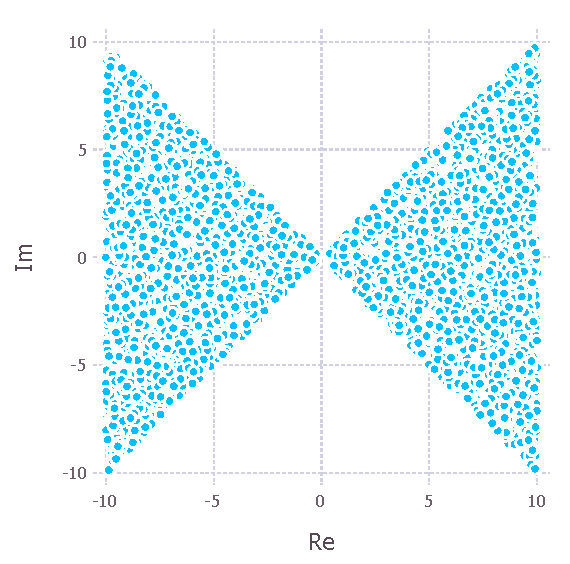
\includegraphics[width=1\linewidth]{contourSimulation_n=2_a=1_cropped.pdf}
      \caption{$n=2$, $a=1$.}
    \end{subfigure}%
    \begin{subfigure}{.5\textwidth}
      \centering
      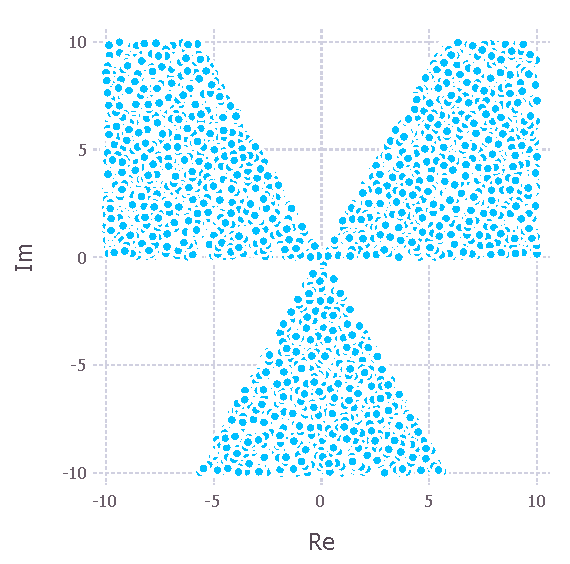
\includegraphics[width=1\linewidth]{contourSimulation_n=3_a=-i_cropped.pdf}
      \caption{$n=3$, $a=-i$.}
    \end{subfigure}
    \begin{subfigure}{.5\textwidth}
        \centering
        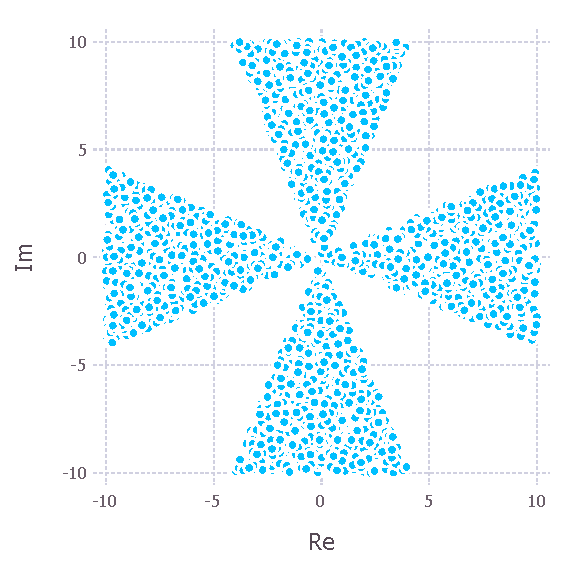
\includegraphics[width=1\linewidth]{contourSimulation_n=4_a=1_cropped.pdf}
        \caption{$n=4$, $a=1$.}
    \end{subfigure}
    \begin{subfigure}{.5\textwidth}
        \centering
        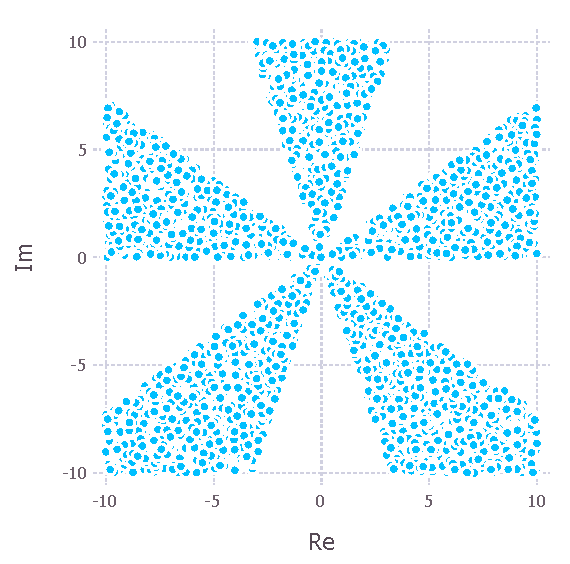
\includegraphics[width=1\linewidth]{contourSimulation_n=5_a=-i_cropped.pdf}
        \caption{$n=5$, $a=-i$.}
    \end{subfigure}
    \caption{Simulation of the region $\{\lambda\in\C:\,\real(a\lambda^n)>0\}$ by randomly sampling $10^4$ points $\lambda$ and keeping those that satisfy $\real(a\lambda^n)>0$.}
    \label{fig:contourTracing}
\end{figure}

\paragraph{Deforming contour backbone to avoid poles of the integrands}\label{sec:deform_contours}\mbox{}\\
The boundaries of the sectors found above form the ``backbones'' of the contours $\Gamma_a^+$ and $\Gamma_a^-$. We proceed to turn these ``backbones'' into $\Gamma_a^+$, $\Gamma_a^-$ by deforming them to avoid  the poles of the integrands $F^+_\lambda$ and $F^-_\lambda$, i.e., the zeros of $\Delta(\lambda)$. 

Before going into the technicalities of the contour deformation, we first draw attention to a modification of the mathematical construction of $\Gamma$ in the actual implementation of the algorithm. In \eqref{eq:gamma}, $\Gamma$ is defined on the entire complex plane; that is, we can have $\lambda$ with arbitrarily large modulus. In the actual implementation, however, we choose a sufficiently large real number $d$ to represent the modulus of complex infinity in the algorithm's context. That is, we restrict the mathematical construction to the disk $D(0, d)$. As the choice of $d$ potentially implies a tradeoff between computational cost and numerical accuracy, it should be chosen with regard to the error tolerance of the computational task at hand. The figures in this report and the documentation of the implementation of the Fokas method \cite{Xiao} are obtained with $d=10$ for clearer illustration. Note that the original infinite contour integrals are understood as improper integrals which, whenever they exist, are equal to their principal values, namely the limits of the respective integrals as the integration bounds tend to infinity. Truncating within $D(0,d)$ and expecting convergence as $d\to\infty$ is therefore legitimate.

By the theory of exponential polynomials \cite{Langer1931}, $\Delta(\lambda)$ has infinitely many zeros, yet any finite region contains only finitely many of these zeros. Since we restrict the construction to the finite region $D(0, d)$, we would only be dealing with finitely many zeros of $\Delta(\lambda)$. This is an important fact: One complication that arises in practice is that each circular contour around a zero of $\Delta(\lambda)$ not only cannot overlap with the circle around another zero but also cannot overlap with the boundary of any sector. That is, in Figure \ref{fig:gamma_smith_fokas}, the blue and black circles not only cannot overlap with each other, but they also cannot overlap with the red or green dashed lines if the zeros of $\Delta(\lambda)$ at their centers do not lie on the boundaries of the red or green sectors. This implies that the $5\epsilon$ introduced in section \ref{sec:fokas_transform_pair} in fact needs to be the minimum of the infimum of the pairwise distances between distinct zeros of $\Delta(\lambda)$ and the infimum of distances between each zero that is exterior to all sectors and the boundary of each sector. The theory of exponential polynomials \cite{Langer1931} guarantees that the former infimum is positive, but there is no such guarantee for the latter infimum. However, precisely because we are working with a finite number of zeros of $\Delta(\lambda)$ in $D(0, d)$, the latter infimum is indeed positive, and so is $\epsilon$. 

To see that our choice of $\epsilon$ is valid, suppose $5\epsilon$ is the minimum of the two infima described above. Then the circle of radius $\epsilon$ around a zero of $\Delta(\lambda)$ does not overlap with any sector boundary. Moreover, the contours around any two distinct zeros of $\Delta(\lambda)$ do not overlap. Indeed: In Figure \ref{fig:epsilon}, suppose the radius of the blue circle around a zero of $\Delta(\lambda)$ is $\epsilon$ and the distance between the blue circle and the red dashed curve around it is again $\epsilon$. Then since the distance between any two distinct zeros of $\Delta(\lambda)$ is no less than $5\epsilon$, the blue circle together with the red dashed curve around it is still of distance $5\epsilon-2\epsilon\cdot 2 = \epsilon$ from the red dashed curve and the blue circle surrounding the nearest zero of $\Delta(\lambda)$. Thus, our choice of $\epsilon$ ensures that no contour around a zero of $\Delta(\lambda)$ is ``overwritten'' by the contour around another zero.

\begin{figure}[htpb!]
    \centering
    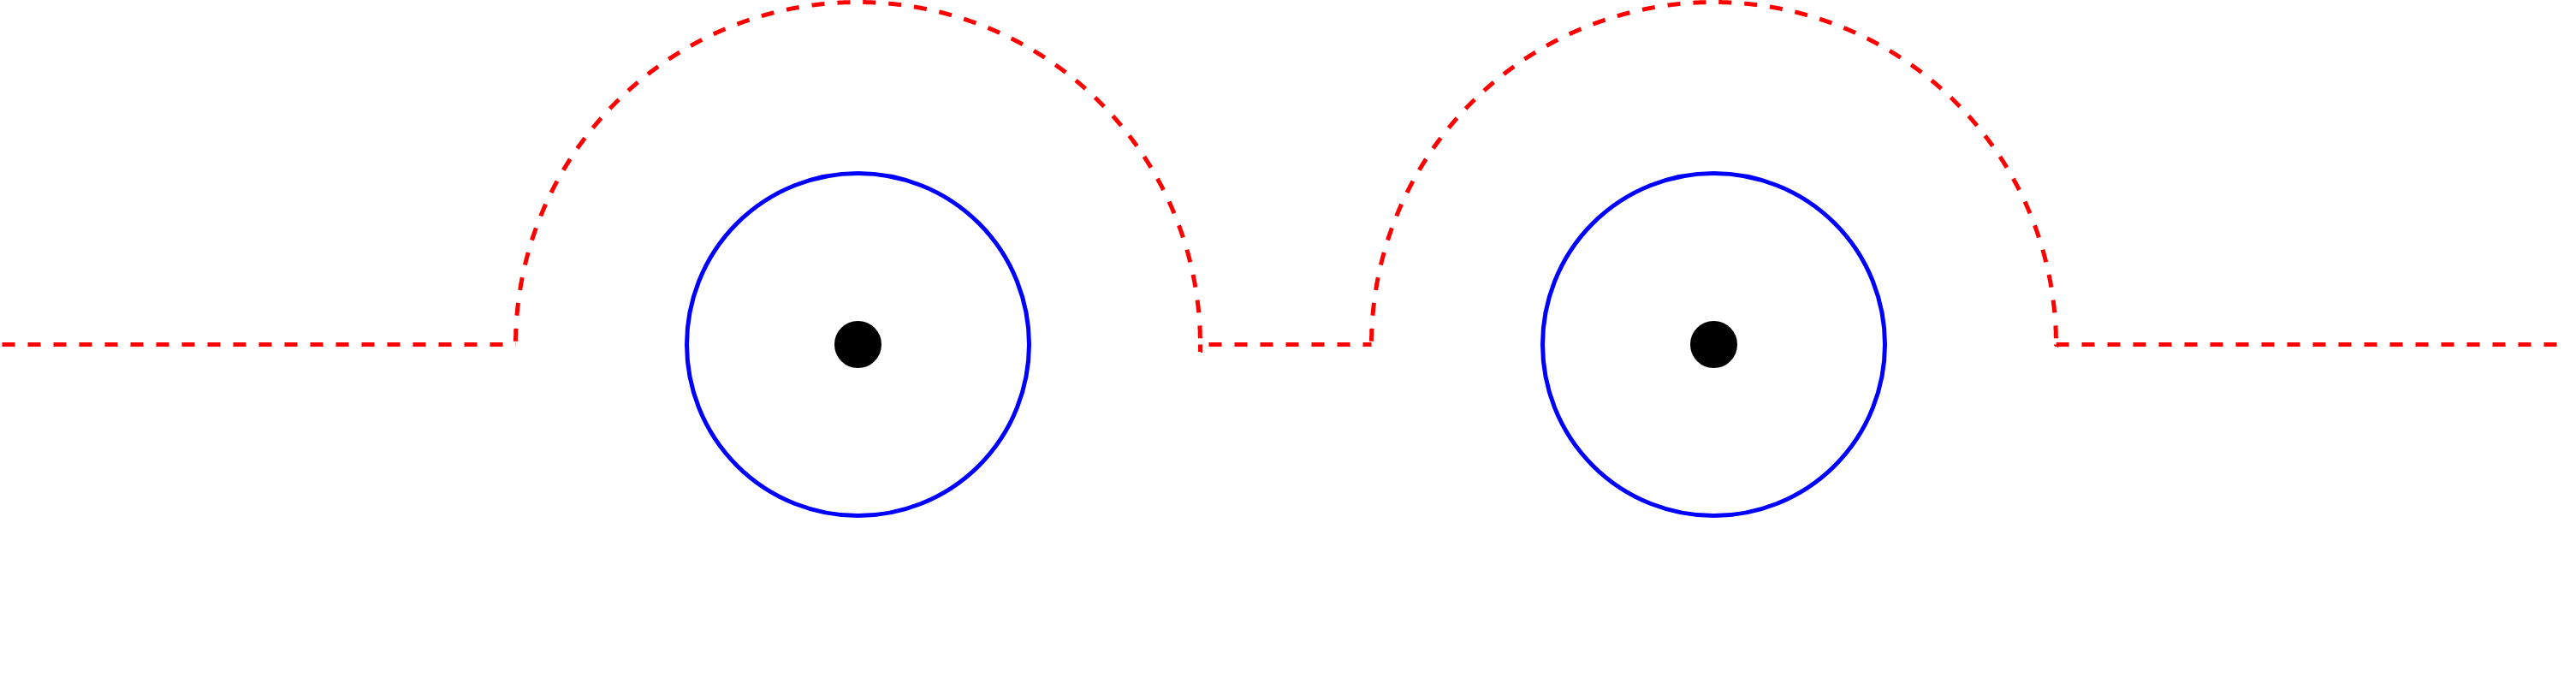
\includegraphics[width=0.8\textwidth]{epsilon_ps.png}
    \caption{Two distinct zeros of $\Delta(\lambda)$ (black dots) that are $5\epsilon$ apart. The blue circles and red dashed contours are as in Figure \ref{fig:gamma_smith_fokas}. The radius of the blue circles, the distance between each blue circle and the red dashed curve around it, and the distance between the two red dashed curves, are all $\epsilon$.}
    \label{fig:epsilon}
\end{figure}

Suppose for now that we have been given finitely many zeros of $\Delta(\lambda)$ in $D(0, d)$ (we will show how to approximate these zeros at the end of this section).

In the complex plane, a ray (straight half-line) emanating from the origin is characterized by the argument of any point on the ray. From Figure \ref{fig:contourTracing}, we note that each sector in the region $\{\lambda\in\C:\, \real(a\lambda^n)>0\}$ is characterized by the arguments of the two rays that mark its boundaries, namely the starting ray and the ending ray, such that if the sector is traversed counterclockwise from one end to the other, the starting ray will be traversed before the ending ray. For example, with $n=3$ and $a=-i$, as shown in section \ref{par:tracing_contour_sectors}, the region $\{\lambda\in\C:\, \real(a\lambda^n)>0\}$ is characterized by the rays with arguments $0, \frac{\pi}{3}, \frac{2}{3}\pi, \pi, \frac{4}{3}\pi, \frac{5}{3}\pi$, where $0, \frac{2}{3}\pi, \frac{4}{3}\pi$ are the angles of the starting rays, and $\frac{\pi}{3}, \pi, \frac{5}{3}\pi$ are the angles of the ending rays. 

Note that each sector is assigned to $\Gamma_a^+$ or $\Gamma_a^-$ depending on whether it belongs to the upper or the lower half plane. As shown in Figure \ref{fig:contourPlot_n=2}, if a sector overlaps with the real line, we divide it into the upper and lower half planes, which can then be assigned to $\Gamma_a^+$ and $\Gamma_a^-$, respectively. In the implementation, this is done by modifying the starting and ending rays that characterize the sector so that the sector is split into two sub-sectors, one ending at the real line and the other starting at it.

The contours $\Gamma_a^\pm$ are built from these rays with possible deformations to avoid zeros of $\Delta(\lambda)$. Here we make another modification of the mathematical construction in \eqref{eq:gamma} to save computational cost. We note that the contours $\Gamma_a^\pm$ and $\Gamma_0^\pm$ defined in \eqref{eq:gamma} lead to partial cancellation, and deformation is in fact only necessary if a zero lies on the boundary of some sector. Indeed: As illustrated in Figure \ref{fig:gamma_smith_fokas}, the red and blue dashed lines do not need to be deformed to avoid zeros exterior to all sectors because they are already outside the sectors. Moreover, zeros interior to any sector can be ignored, since integrating over the blue circle around the zero counterclockwise cancels with integrating over the interior red dashed circle around the zero clockwise. For a zero that lies on the boundary of the sector, half of the blue circle around it that is interior to the sector cancels out with the red dashed curve around it, but the other half that is exterior to the sector does not cancel with anything. In this case, we deform the ray on which the zero lies to include the exterior half of the blue circle that does not cancel. 

On a side note, the way we deform the contours described above implies that we can choose $\epsilon$ to be $\frac{1}{4}$ the minimum of the pairwise distances between distinct zeros of $\Delta(\lambda)$ and the distances between any zero to any sector boundary, instead of $\frac{1}{5}$ as in section \ref{sec:contour_defn}. Indeed: Since we have merged the blue circle into the red dashed curve in the previous paragraph, the scenario in Figure \ref{fig:epsilon} would not occur. Instead, the scenario that puts the most constraint on $\epsilon$ occurs when a zero is at the origin, and as shown in Figure \ref{fig:epsilon_2}, this scenario only requires that the two distinct zeros are $4\epsilon$ apart. Besides mathematical clarity, there is a subtlety in the implementation that actually argues for using $4\epsilon$ over $5\epsilon$: Since zeros of $\Delta(\lambda)$ are poles of the integrands $F_\lambda^+$, $F_\lambda^-$ in \eqref{eq:F_lambda_+-}, the values of $F_\lambda^+$, $F_\lambda^-$ easily blow up near the zeros, thereby creating numerical instability that could make integration very slow. Thus, we use the new choice of $\epsilon$ in the actual implementation to make the contours stay further away from the zeros. Figure \ref{fig:contourPlots} shows the contour $\Gamma$ for some examples, and Figure \ref{fig:contourPlot_n=2} shows each component of $\Gamma$ of Figure \ref{fig:contourPlots}(a) separately.

\begin{figure}[htpb!]
    \centering
    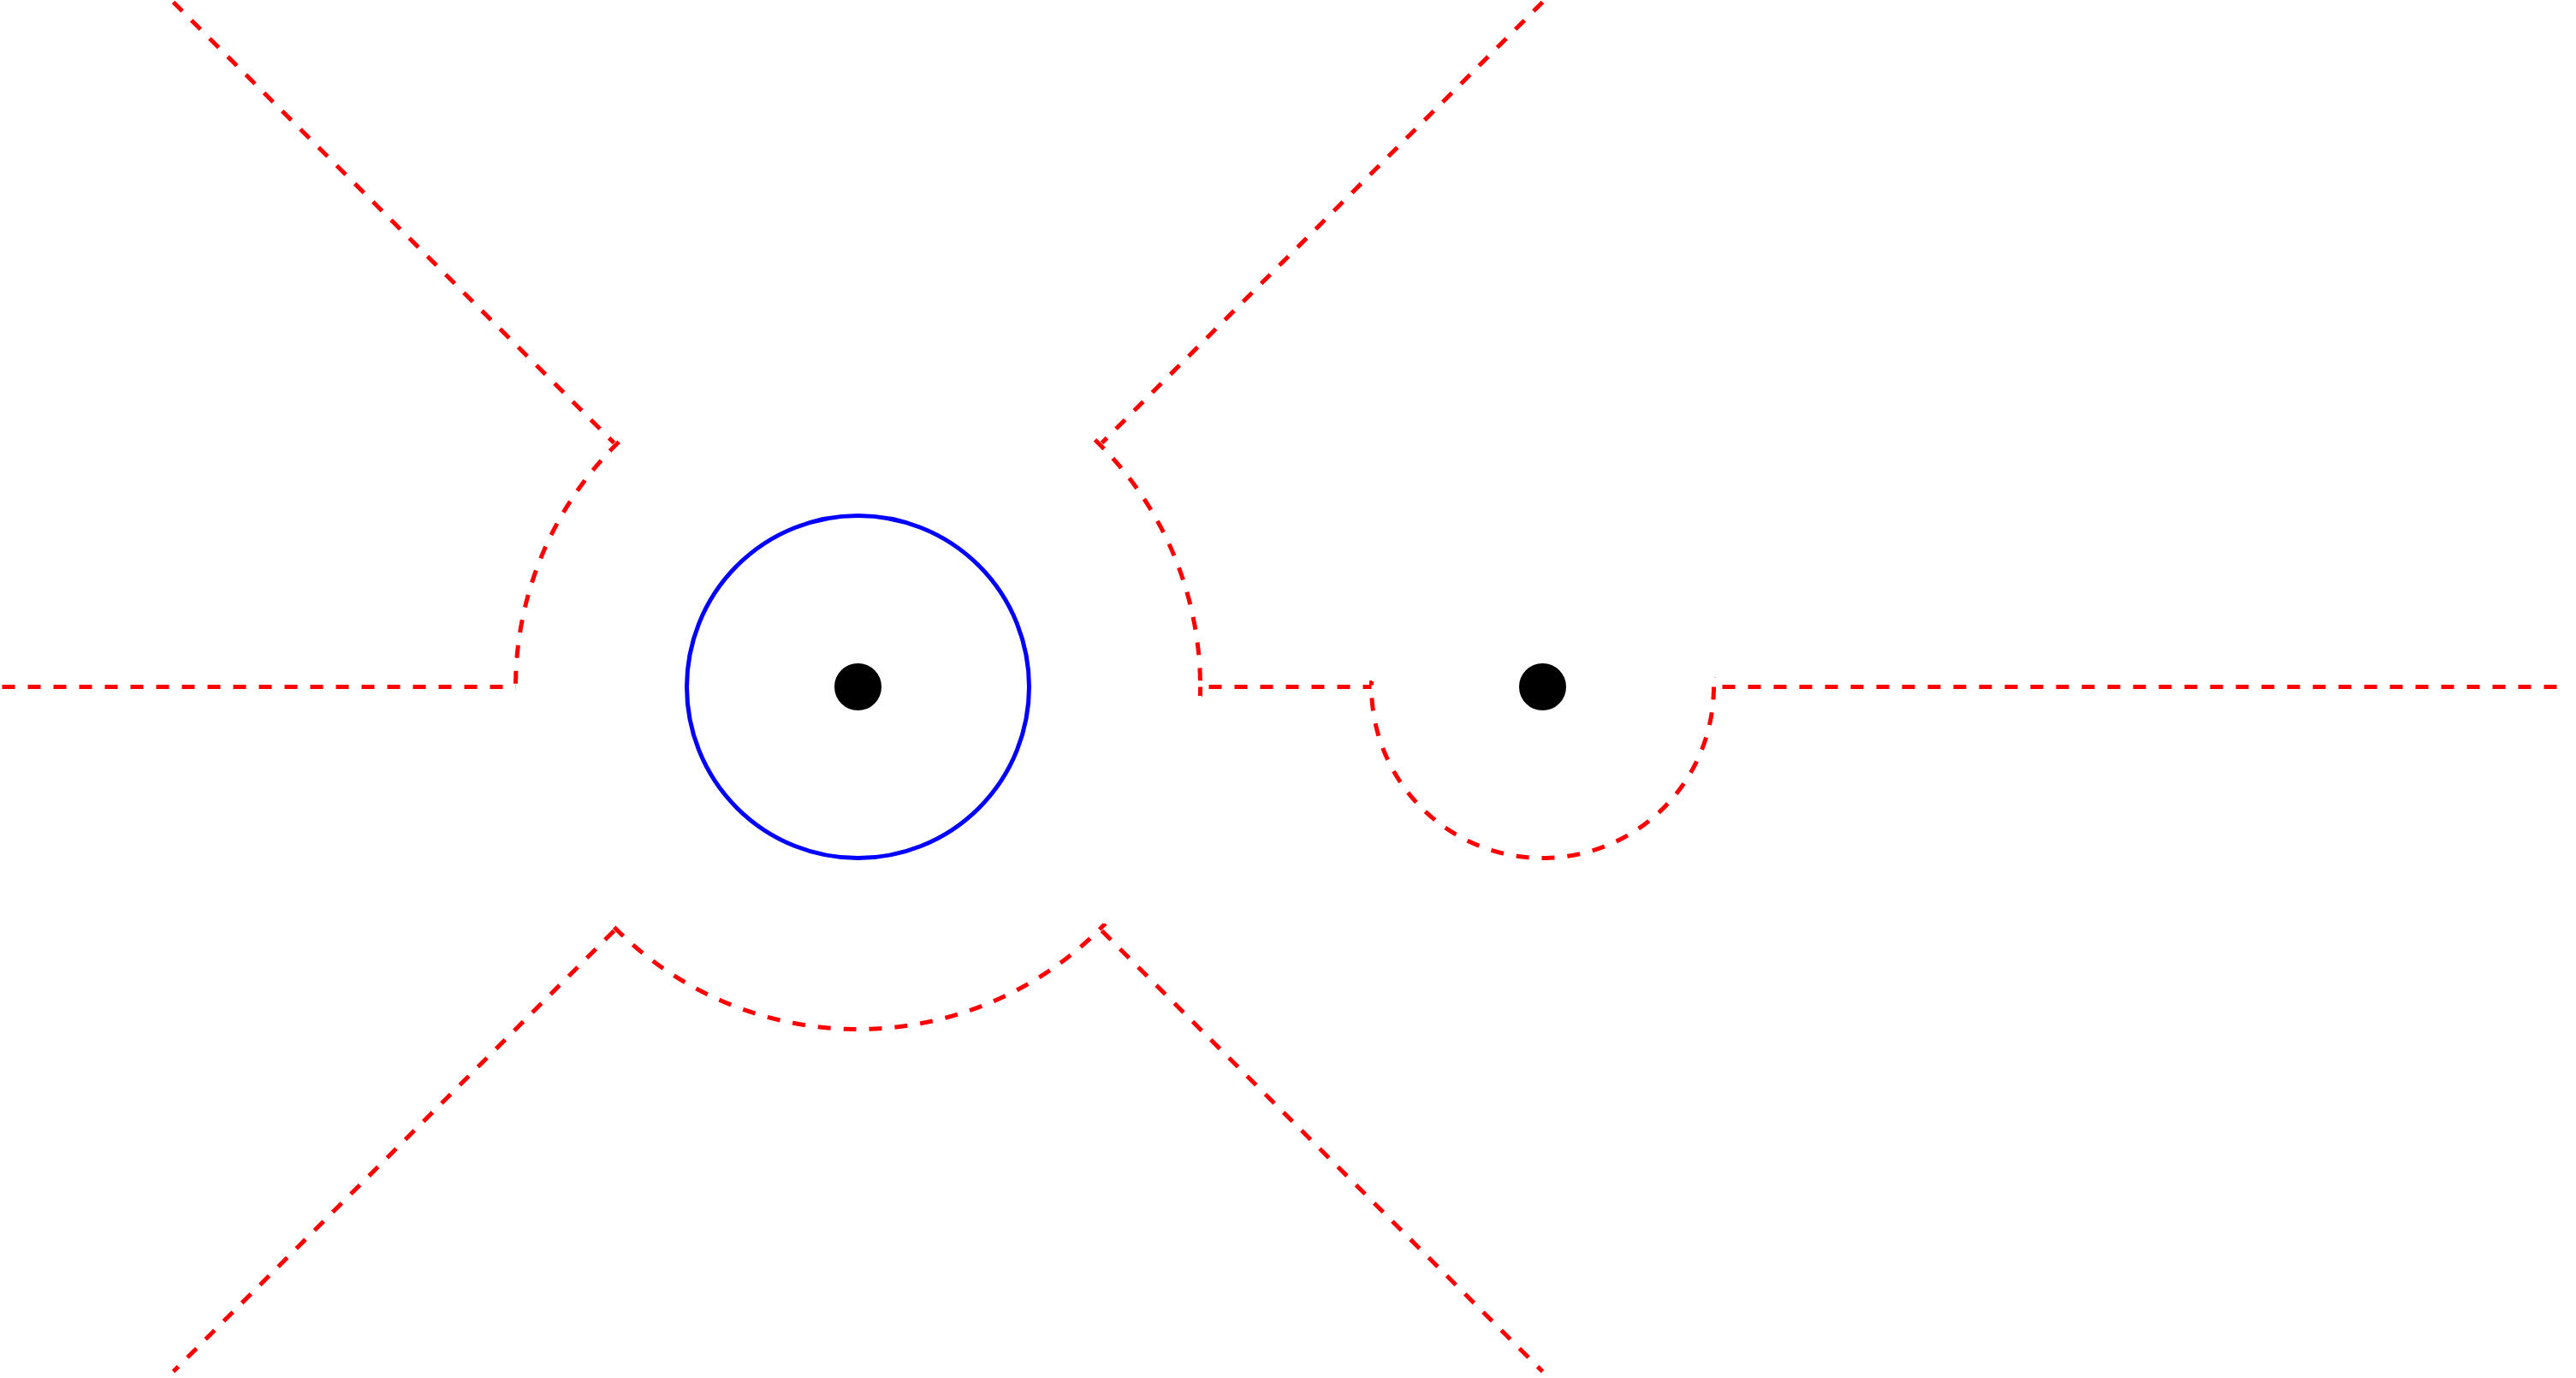
\includegraphics[width=0.8\textwidth]{epsilon_2_ps.png}
    \caption{Two distinct zeros of $\Delta(\lambda)$ (black dots) that are $4\epsilon$ apart. The zero on the left is at the origin. The blue circles and red dashed contours are as in Figure \ref{fig:gamma_smith_fokas} (though not drawn to scale here). The radius of the blue circle, the distance between the blue circle and the red dashed curve around it, and the distance between the red dashed curve around the blue circle and the red dashed curve around the zero on the right, are all $\epsilon$.}
    \label{fig:epsilon_2}
\end{figure}


\begin{figure}[htpb!]
    \begin{subfigure}{.5\textwidth}
      \centering
      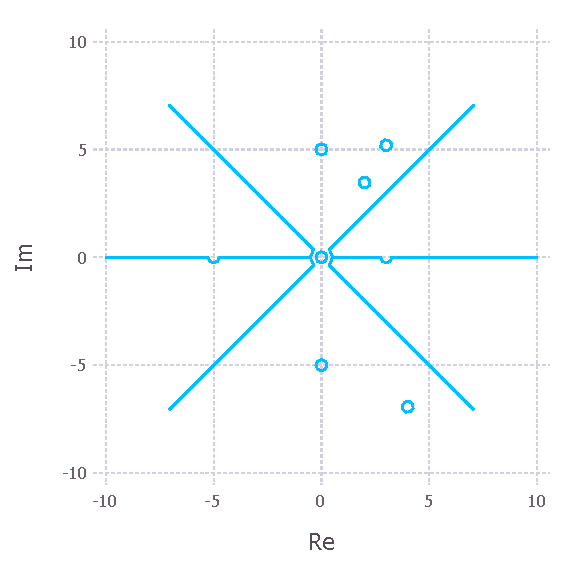
\includegraphics[width=1\linewidth]{contourPlot_n=2_a=1_cropped.pdf}
      \caption{$n=2$, $a=1$.}
    \end{subfigure}%
    \begin{subfigure}{.5\textwidth}
      \centering
      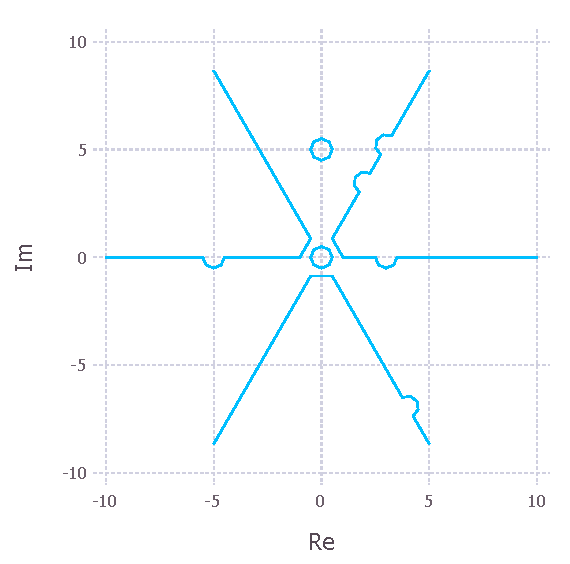
\includegraphics[width=1\linewidth]{contourPlot_n=3_a=-i_cropped.pdf}
      \caption{$n=3$, $a=-i$.}
    \end{subfigure}
    \begin{subfigure}{.5\textwidth}
        \centering
        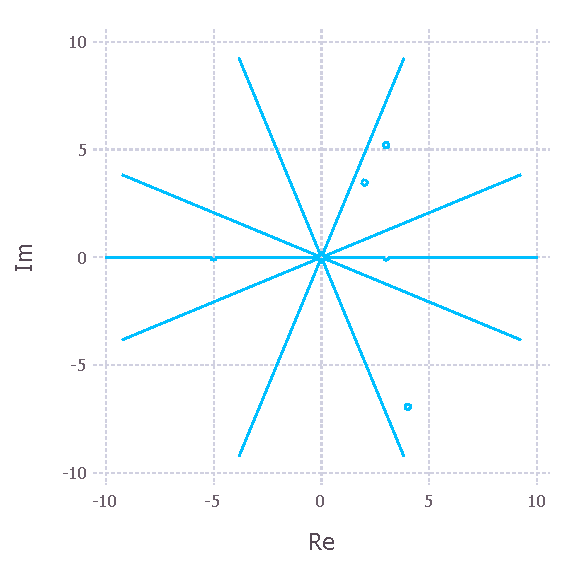
\includegraphics[width=1\linewidth]{contourPlot_n=4_a=1_cropped.pdf}
        \caption{$n=4$, $a=1$.}
    \end{subfigure}
    \begin{subfigure}{.5\textwidth}
        \centering
        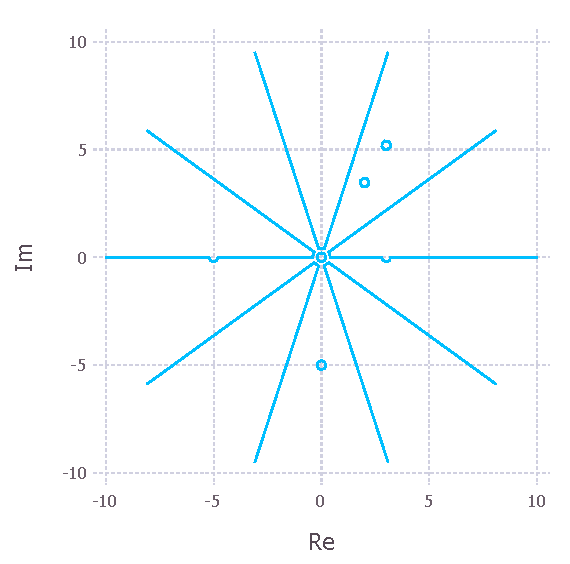
\includegraphics[width=1\linewidth]{contourPlot_n=5_a=-i_cropped.pdf}
        \caption{$n=5$, $a=-i$.}
    \end{subfigure}
    \caption{$\Gamma$ with with zeros of $\Delta(\lambda)$ at $3+3\sqrt{3}i$, $2+2\sqrt{3}i$, $0+0i$, $0+5i$, $0-5i$, $3$, $-5$, and $4-4\sqrt{3}i$. Note that $\Gamma_a^+$ are deformed to avoid zeros on the sectors' boundaries.}
    \label{fig:contourPlots}
\end{figure}

\begin{figure}[htpb!]
    \begin{subfigure}{.5\textwidth}
      \centering
      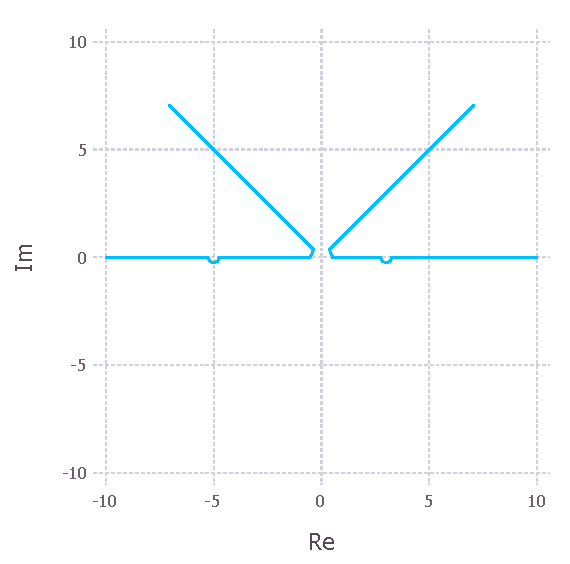
\includegraphics[width=1\linewidth]{contourPlot_n=2_a=1_gammaAPlus_cropped.pdf}
      \caption{$\Gamma_a^+$.}
    \end{subfigure}%
    \begin{subfigure}{.5\textwidth}
      \centering
      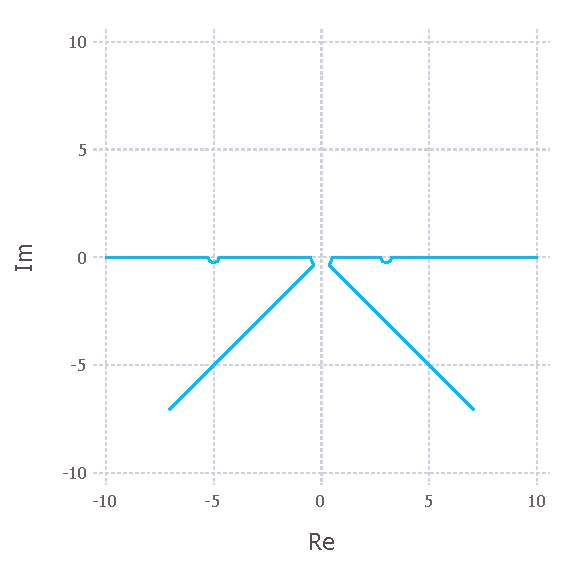
\includegraphics[width=1\linewidth]{contourPlot_n=2_a=1_gammaAMinus_cropped.pdf}
      \caption{$\Gamma_a^-$.}
    \end{subfigure}
    \begin{subfigure}{.5\textwidth}
        \centering
        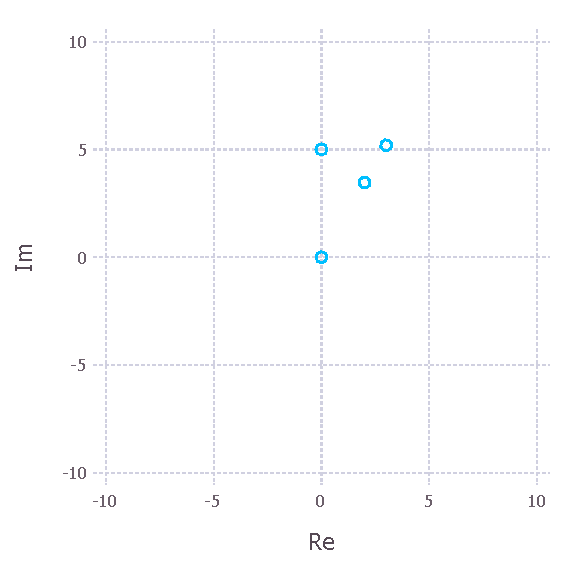
\includegraphics[width=1\linewidth]{contourPlot_n=2_a=1_gamma0Plus_cropped.pdf}
        \caption{$\Gamma_0^+$.}
    \end{subfigure}
    \begin{subfigure}{.5\textwidth}
        \centering
        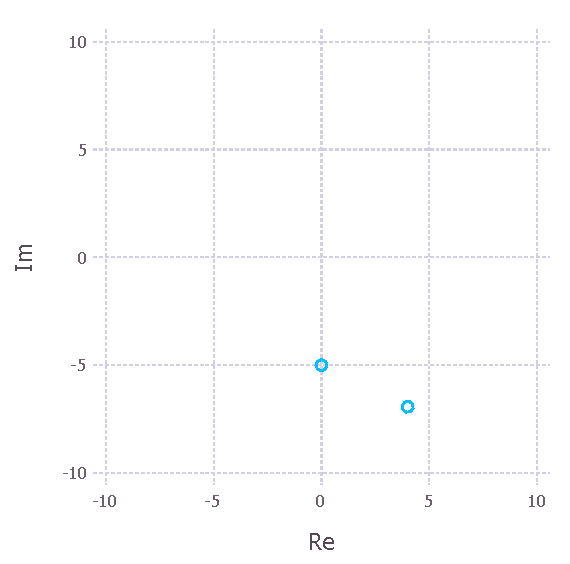
\includegraphics[width=1\linewidth]{contourPlot_n=2_a=1_gamma0Minus_cropped.pdf}
        \caption{$\Gamma_0^-$.}
    \end{subfigure}
    \caption{Components of $\Gamma$ with $n=2$, $a=1$, and the same zeros of $\Delta(\lambda)$ as in Figure \ref{fig:contourPlots}. Note that the sectors are split at the real line into the upper and lower half planes.}
    \label{fig:contourPlot_n=2}
\end{figure}

% The algorithm to construct $\Gamma_a^+$, $\Gamma_a^-$, $\Gamma_0^+$, and $\Gamma_0^-$ is described as follows.
% \begin{algorithm}[H]
%     \caption{Algorithm to construct $\Gamma$.}\label{algo:Find gamma.}
%     \KwData{\texttt{sectors}, \texttt{zeroList}}
%     \KwResult{$\Gamma_a^+$, $\Gamma_a^-$, $\Gamma_0^+$, $\Gamma_0^-$}
%     \Begin{
%         \For{sector in sectors}{
%             sectorContour $\leftarrow$ [sector.startRay, 0, sector.endRay]\;
%             \If{sector in $\C^+$}{
%                 add sector to $\Gamma_a^+$
%             }
%             \Else{
%                 add sector to $\Gamma_a^-$
%             }
%         }
%         sort zeroList by modulus \Comment*[r]{so that the possible zero at the origin comes last}\
%         \For{zero in zeroList}{

%         }
%         mat $\leftarrow$ $(M:N)$\;
%         \For{i in range(nrow(E))}{
%             mat1 $\leftarrow$ vcat(mat, E[i,]) \Comment*[r]{vcat := vertical concatenation, or joining two matrices vertically}\
%             \If{rank(mat1) == rank(mat)+1}{
%                 mat $\leftarrow$ mat1
%             }
%             \Else{
%                 E $\leftarrow$ E[-i,]
%             }
%         }
%         \Return{vcat(mat, E)}
%     }
% \end{algorithm}
The construction of $\Gamma_a^+$, $\Gamma_a^-$, $\Gamma_0^+$, and $\Gamma_0^-$ is described as follows. In the implementation, each contour in $\Gamma$ is encoded by an array of points listed in the order of integration. As shown in Figure \ref{fig:gamma_smith_fokas}, we integrate over each contour in $\Gamma_a^\pm$ from the ending ray to the starting ray, and each contour in $\Gamma_0^\pm$ counterclockwise. Thus, in constructing the contours, for each sector, we initialize its boundary contour by an array of three points, namely the point on the ending ray with modulus $d$, the origin, and the point on the starting ray with modulus $d$. We add these initial sector boundary contours to $\Gamma_a^\pm$ depending on whether the sectors are in the upper or lower half plane. Then, for each zero of $\Delta(\lambda)$ that is not at the origin, if it is on the boundary of some sector, we deform the boundary contour of that sector to include a ``bulge'' that is the exterior half of an $N$-gon of radius $\epsilon$ around the zero, with the vertices listed counterclockwise. If the zero is exterior to all sectors, we add an $N$-gon contour around it to $\Gamma_0^{\pm}$, depending on whether the zero is in the upper or lower half plane. If the zero is interior to any sector, we ignore it, since its contribution to the contour integral will be cancelled out, as explained before. Finally, if there is a zero at the origin, we draw an $N$-gon around it and deform the boundary contours of all sectors to avoid the $N$-gon. 
% At the end of this process, $\Gamma_a$ would contain all sector boundary contours now appropriately deformed, and $\Gamma_0$ would contain all the $N$-gon contours encircling isolated zeros.

\noindent\subparagraph{Approximating poles of the integrands}\mbox{}\label{par:approximating_integrand_poles}\\
As promised, we now describe a method to approximate the poles of $F^+_\lambda$ and $F^-_\lambda$, i.e., the zeros of $\Delta(\lambda)$, in the finite region $D(0,d)$.

Writing $\Delta(\lambda)=\real(\Delta)(\lambda) + i\imag(\Delta)(\lambda)$ for $\real(\Delta), \imag(\Delta): \C\to\R$, we note that $\lambda_0$ is a root of $\Delta(\lambda)$ if and only if it is both a root of $\real(\Delta)(\lambda)$ and a root of $\imag(\Delta)(\lambda)$. Thus, to find zeros of $\Delta(\lambda)$, we aim to solve simultaneously
\begin{subequations}\label{eq:delta_real_imaginary}
    \begin{align}
        \real(\Delta)(\lambda) &= 0,\\
        \imag(\Delta)(\lambda) &= 0.
    \end{align}
\end{subequations}

% We observe that since $\Delta(\lambda)$ is an exponential polynomial of the form
% \[\Delta(\lambda) = \sum_{k=1}^n a_k \lambda^k e^{b_k\lambda},\]
% writing $\lambda=x+iy$ where $x,y\in\R$ gives
% \begin{align*}
%     \Delta(x,y) &= \sum_{k=1}^n a_k (x+iy)^k e^{b_k(x+iy)}\\
%     % &= \sum_{k=1}^n a_k (x+iy)^k e^{b_k x+i b_ky}\\
%     &= \sum_{k=1}^n a_k (x+iy)^k e^{b_k x}(\cos(b_k y) + i\sin(b_k y))\quad\mbox{(Euler's formula)}\\
%     &= \sum_{k=1}^n a_k \left(\sum_{l=0}^k\binom{k}{l}x^{k-l}(iy)^l\right) e^{b_k x}(\cos(b_k y) + i\sin(b_k y))\quad\mbox{(Binomial theorem)}.
% \end{align*}
% Thus, we can always separate the real and imaginary parts of $\Delta(\lambda)$ analytically and find their zeros separately. Therefore, to find the zeros of $\Delta(\lambda)$, it suffices to solve for $x, y$ in 
% \begin{subequations}\label{eq:delta_real_imaginary}
%     \begin{align}
%         \real(\Delta(x, y)) &= 0,\\
%         \imag(\Delta(x, y)) &= 0.
%     \end{align}
% \end{subequations}

We approximate the solutions to \eqref{eq:delta_real_imaginary} by visualizing their corresponding level curves. In the examples shown in Figure \ref{fig:levelCurves}, the red lines correspond to the zeros of $\real(\Delta)(\lambda)$, and the blue lines correspond to those of $\imag(\Delta)(\lambda)$. Thus, We can locate the zeros of $\Delta(\lambda)$ at the intersections of the red and blue lines. 

\begin{figure}[htpb!]
    \begin{subfigure}{.5\textwidth}
      \centering
      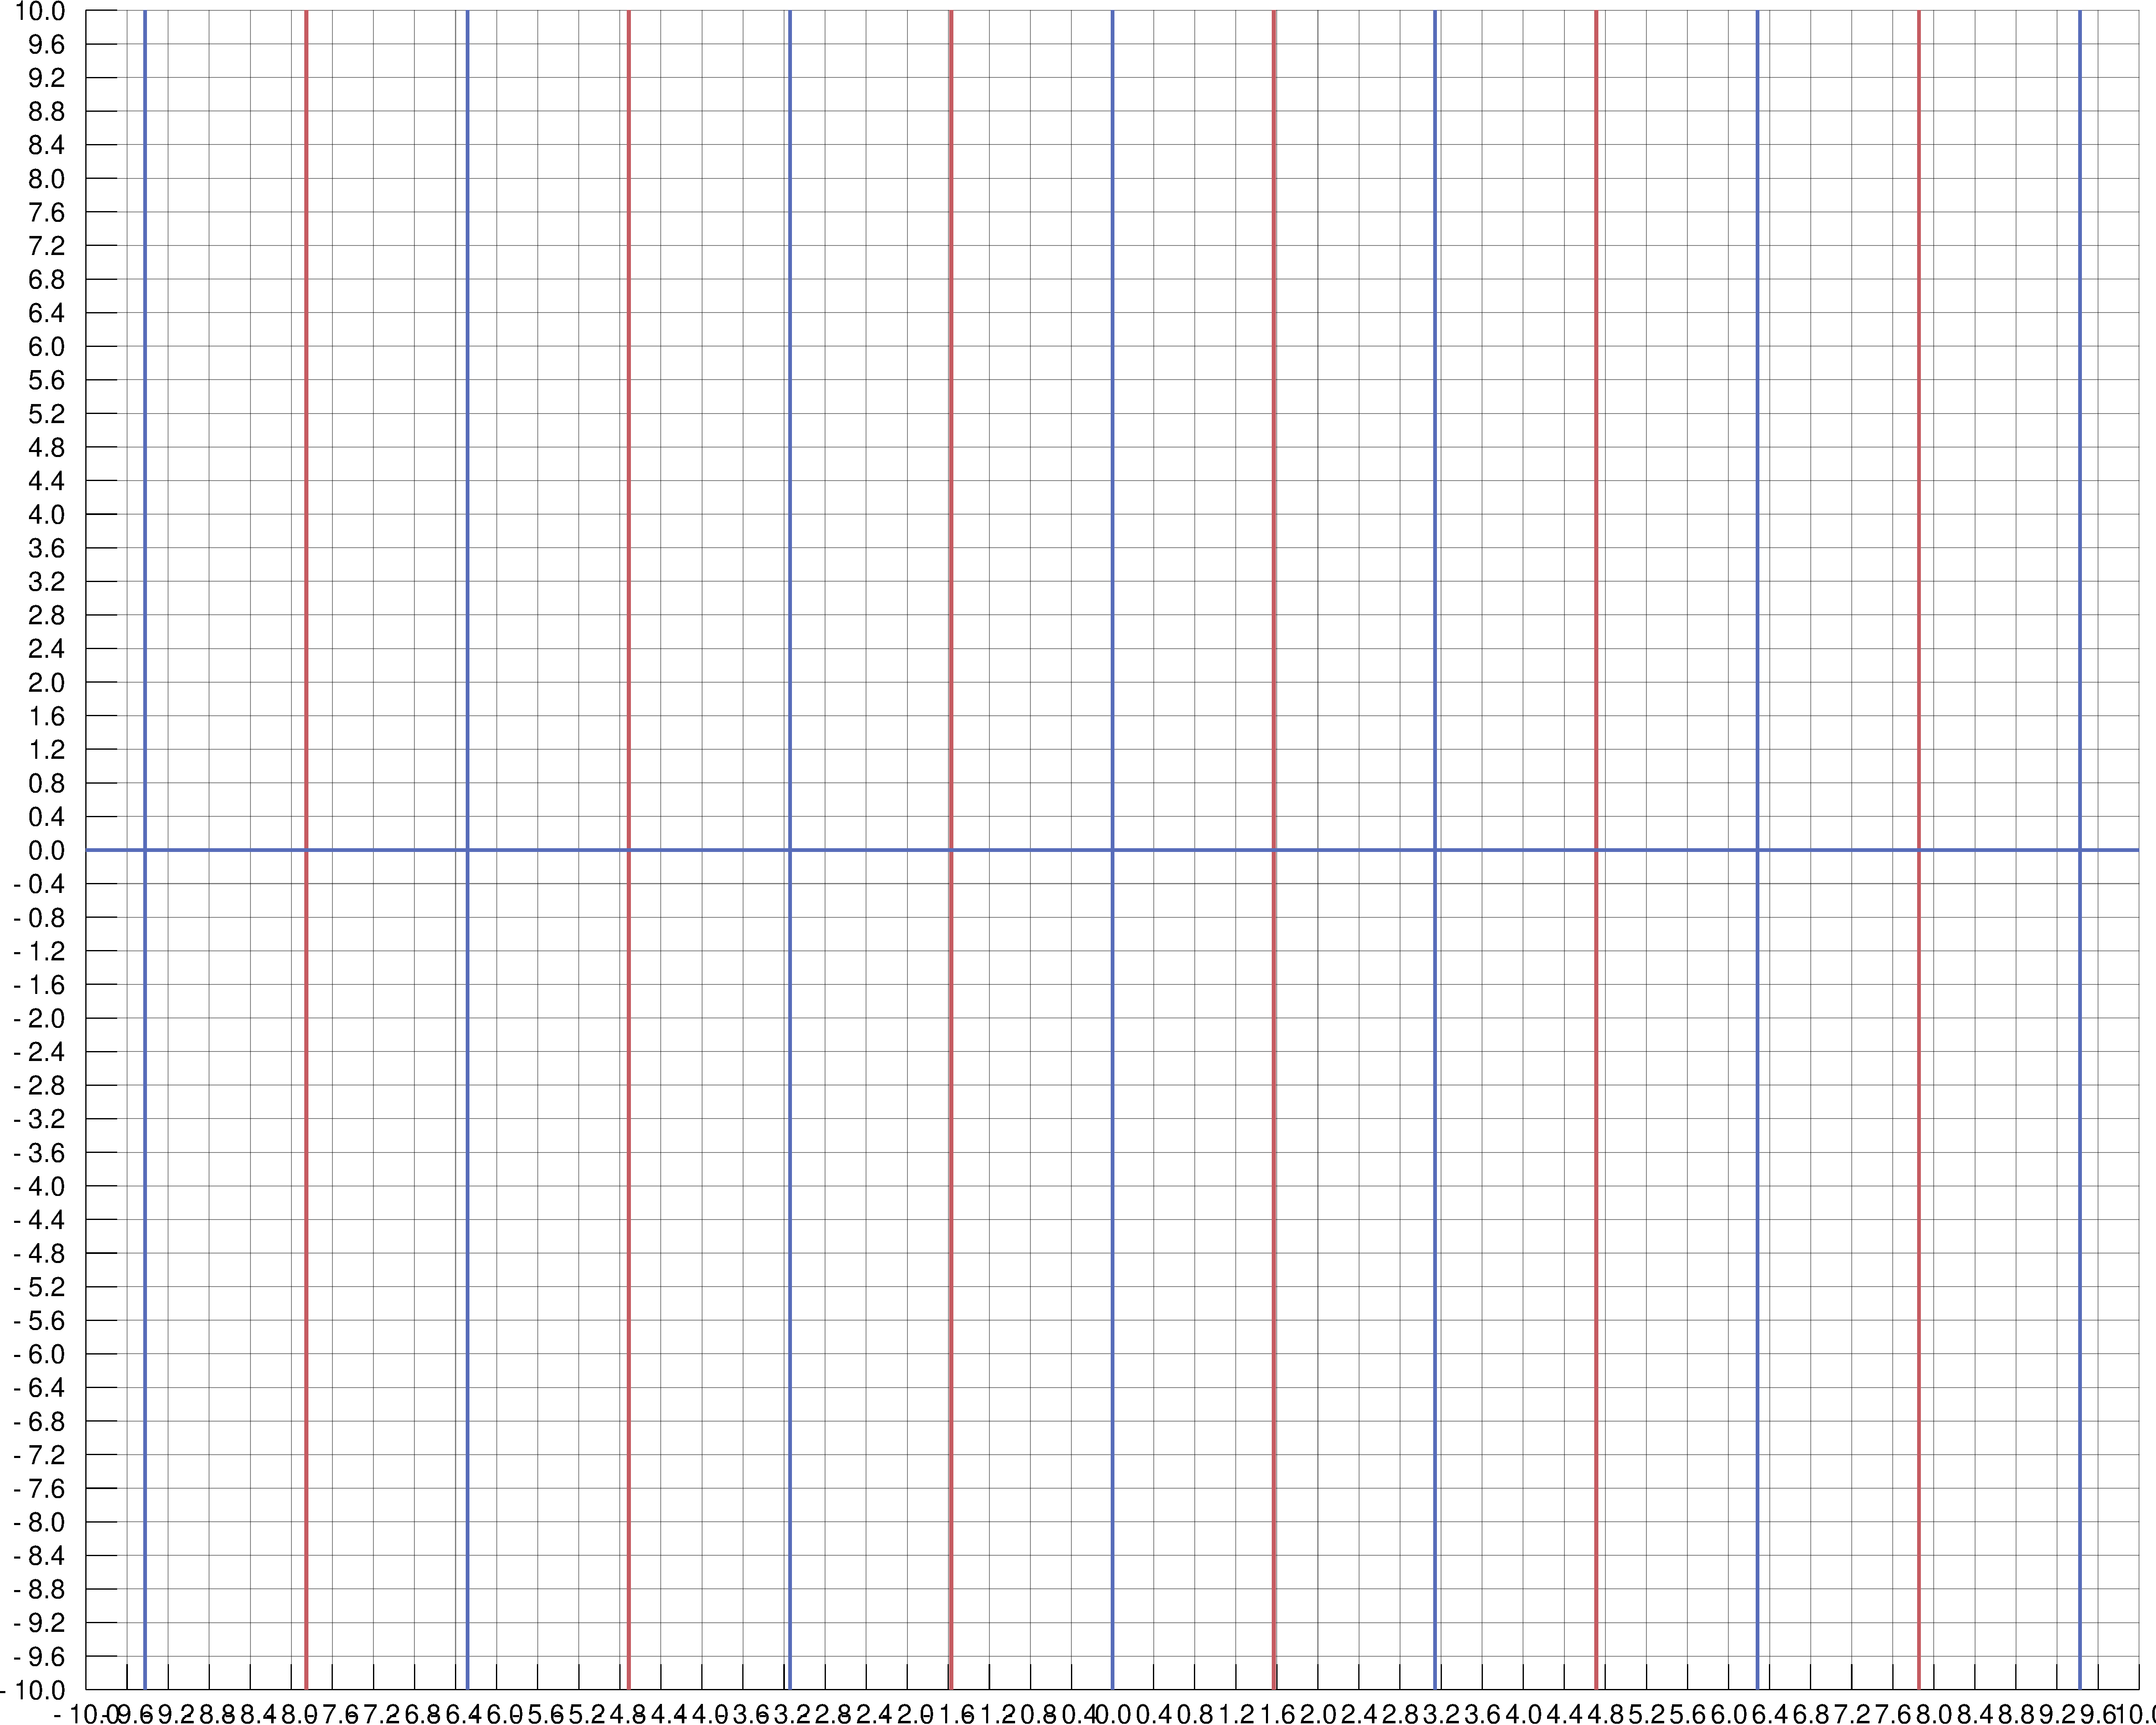
\includegraphics[width=1\linewidth]{levelCurves_1.pdf}
      \caption{$\Delta(\lambda) = \cos(\lambda)$.}
    \end{subfigure}%
    \begin{subfigure}{.5\textwidth}
      \centering
      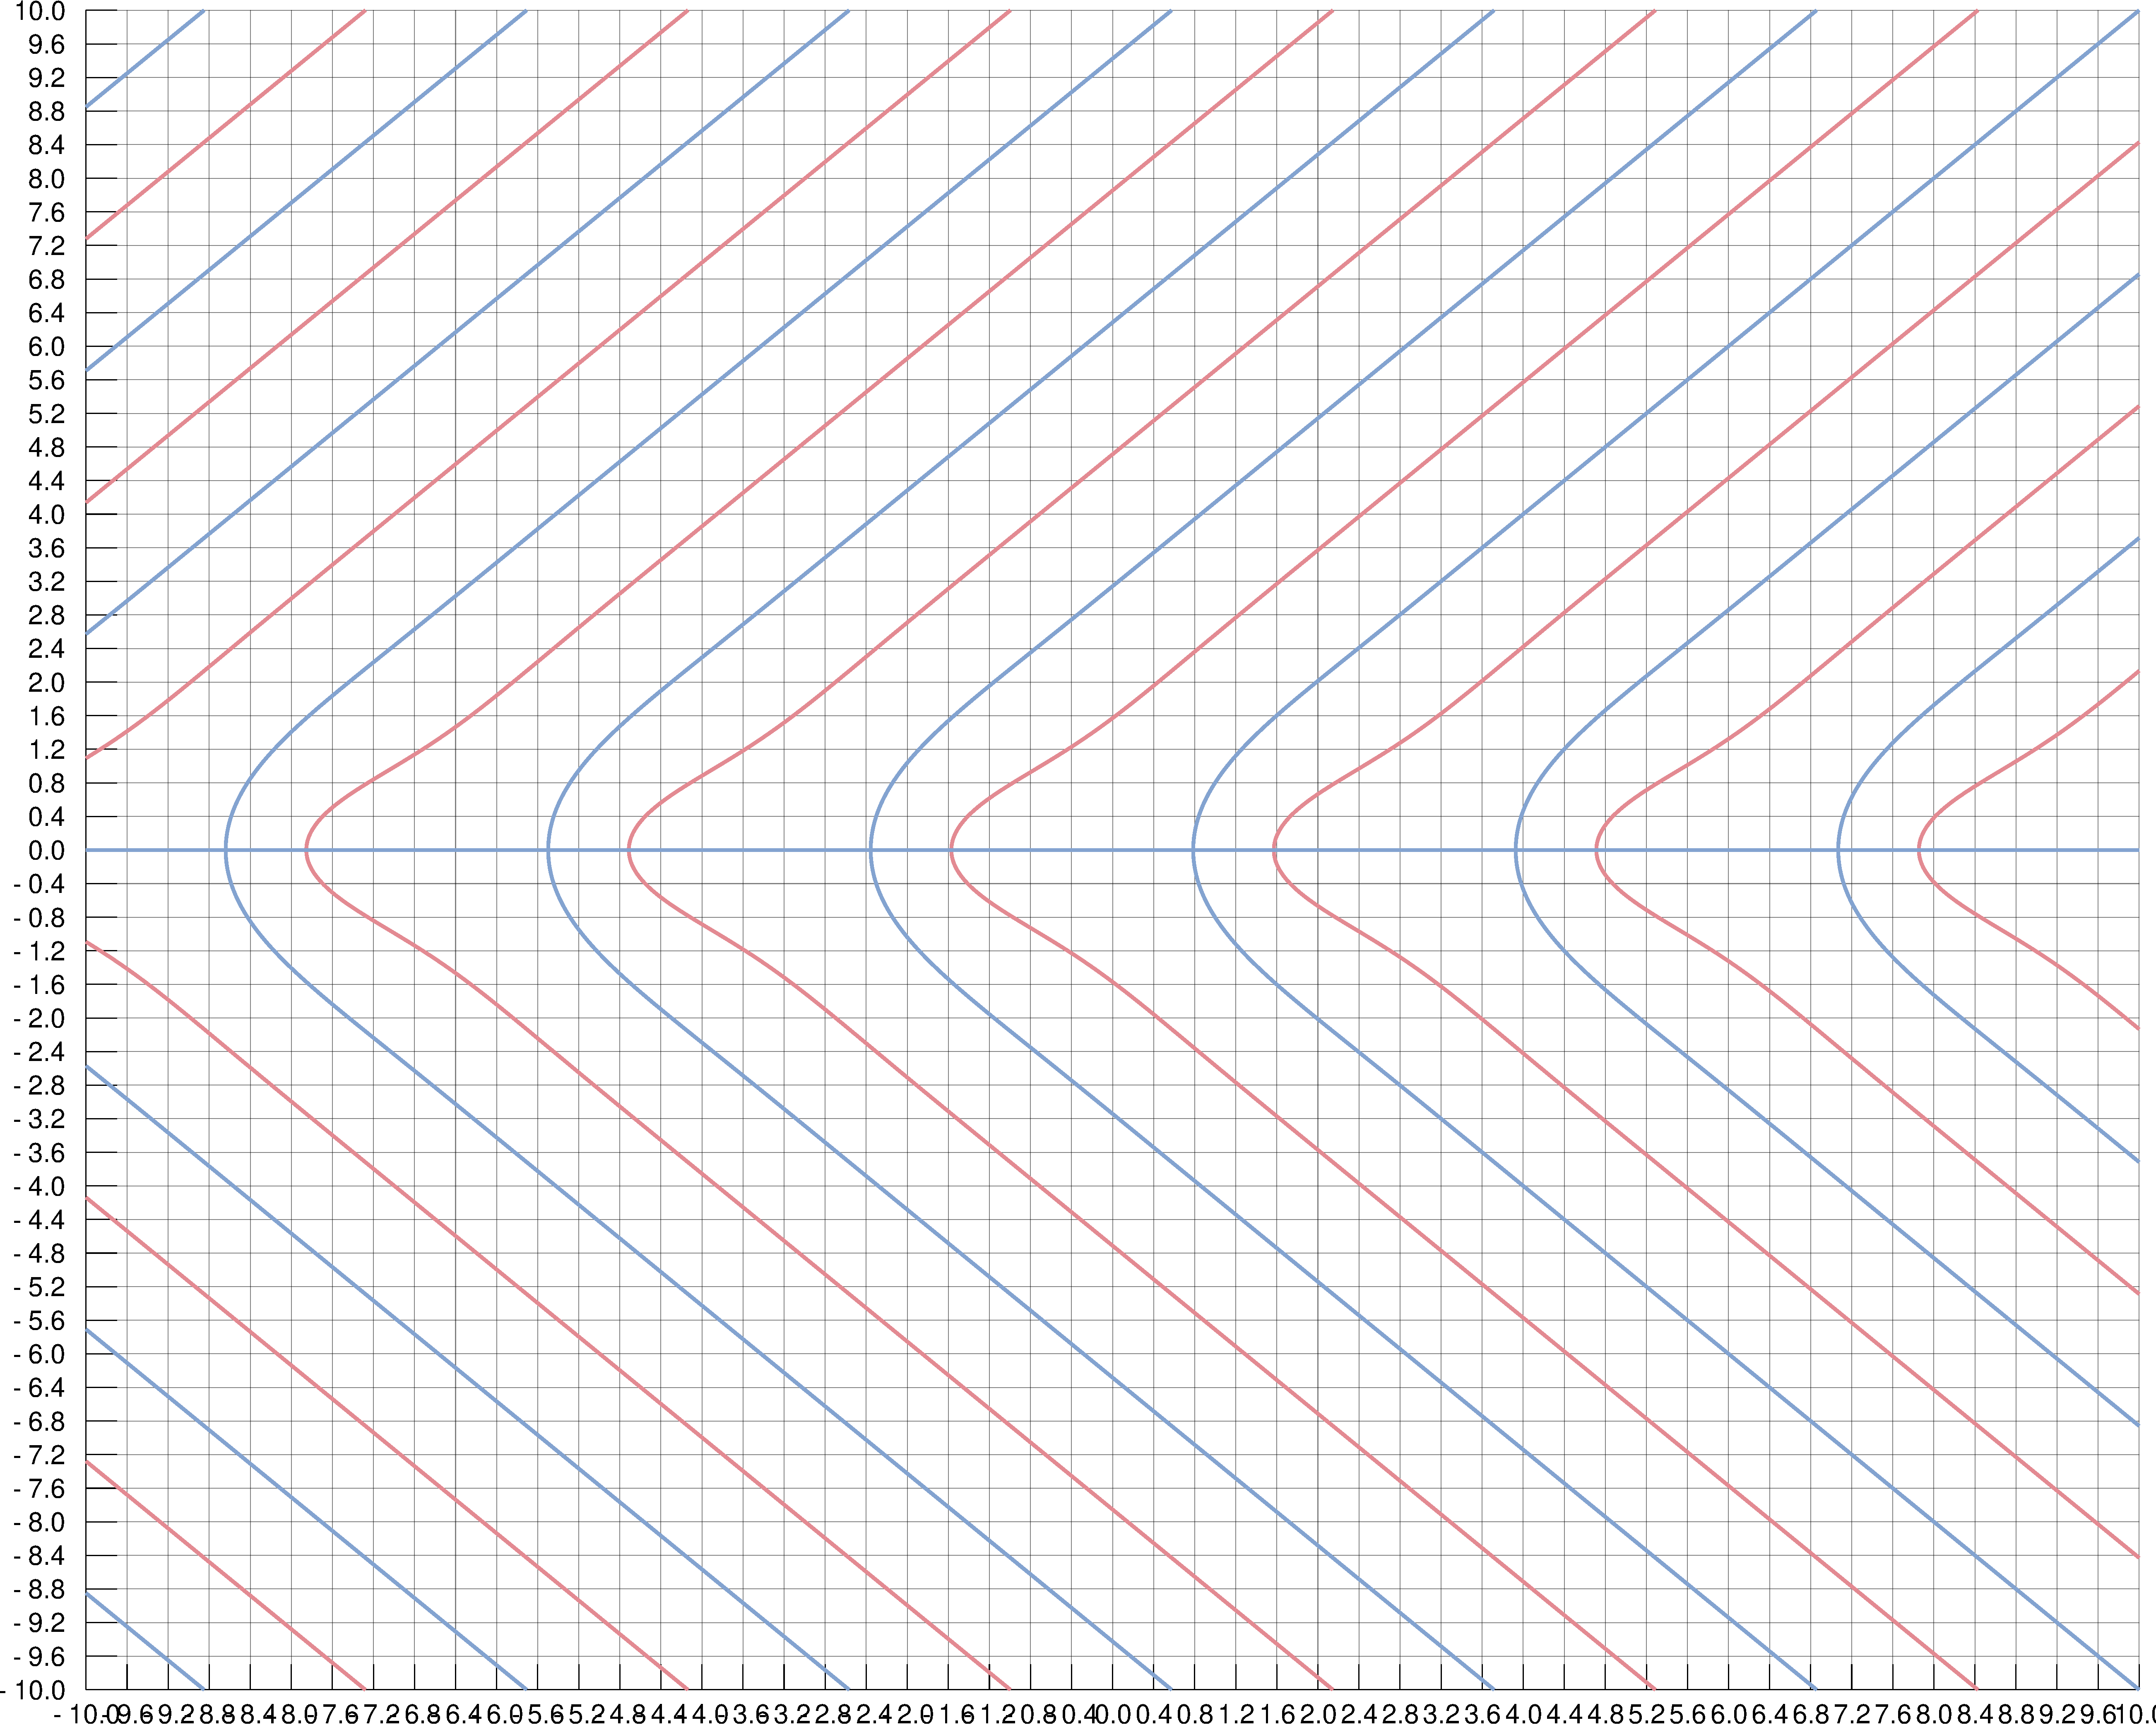
\includegraphics[width=1\linewidth]{levelCurves_2.pdf}
      \caption{$\Delta(\lambda) = \cos(\lambda)e^{\lambda}$.}
    \end{subfigure}
    \begin{subfigure}{.5\textwidth}
        \centering
        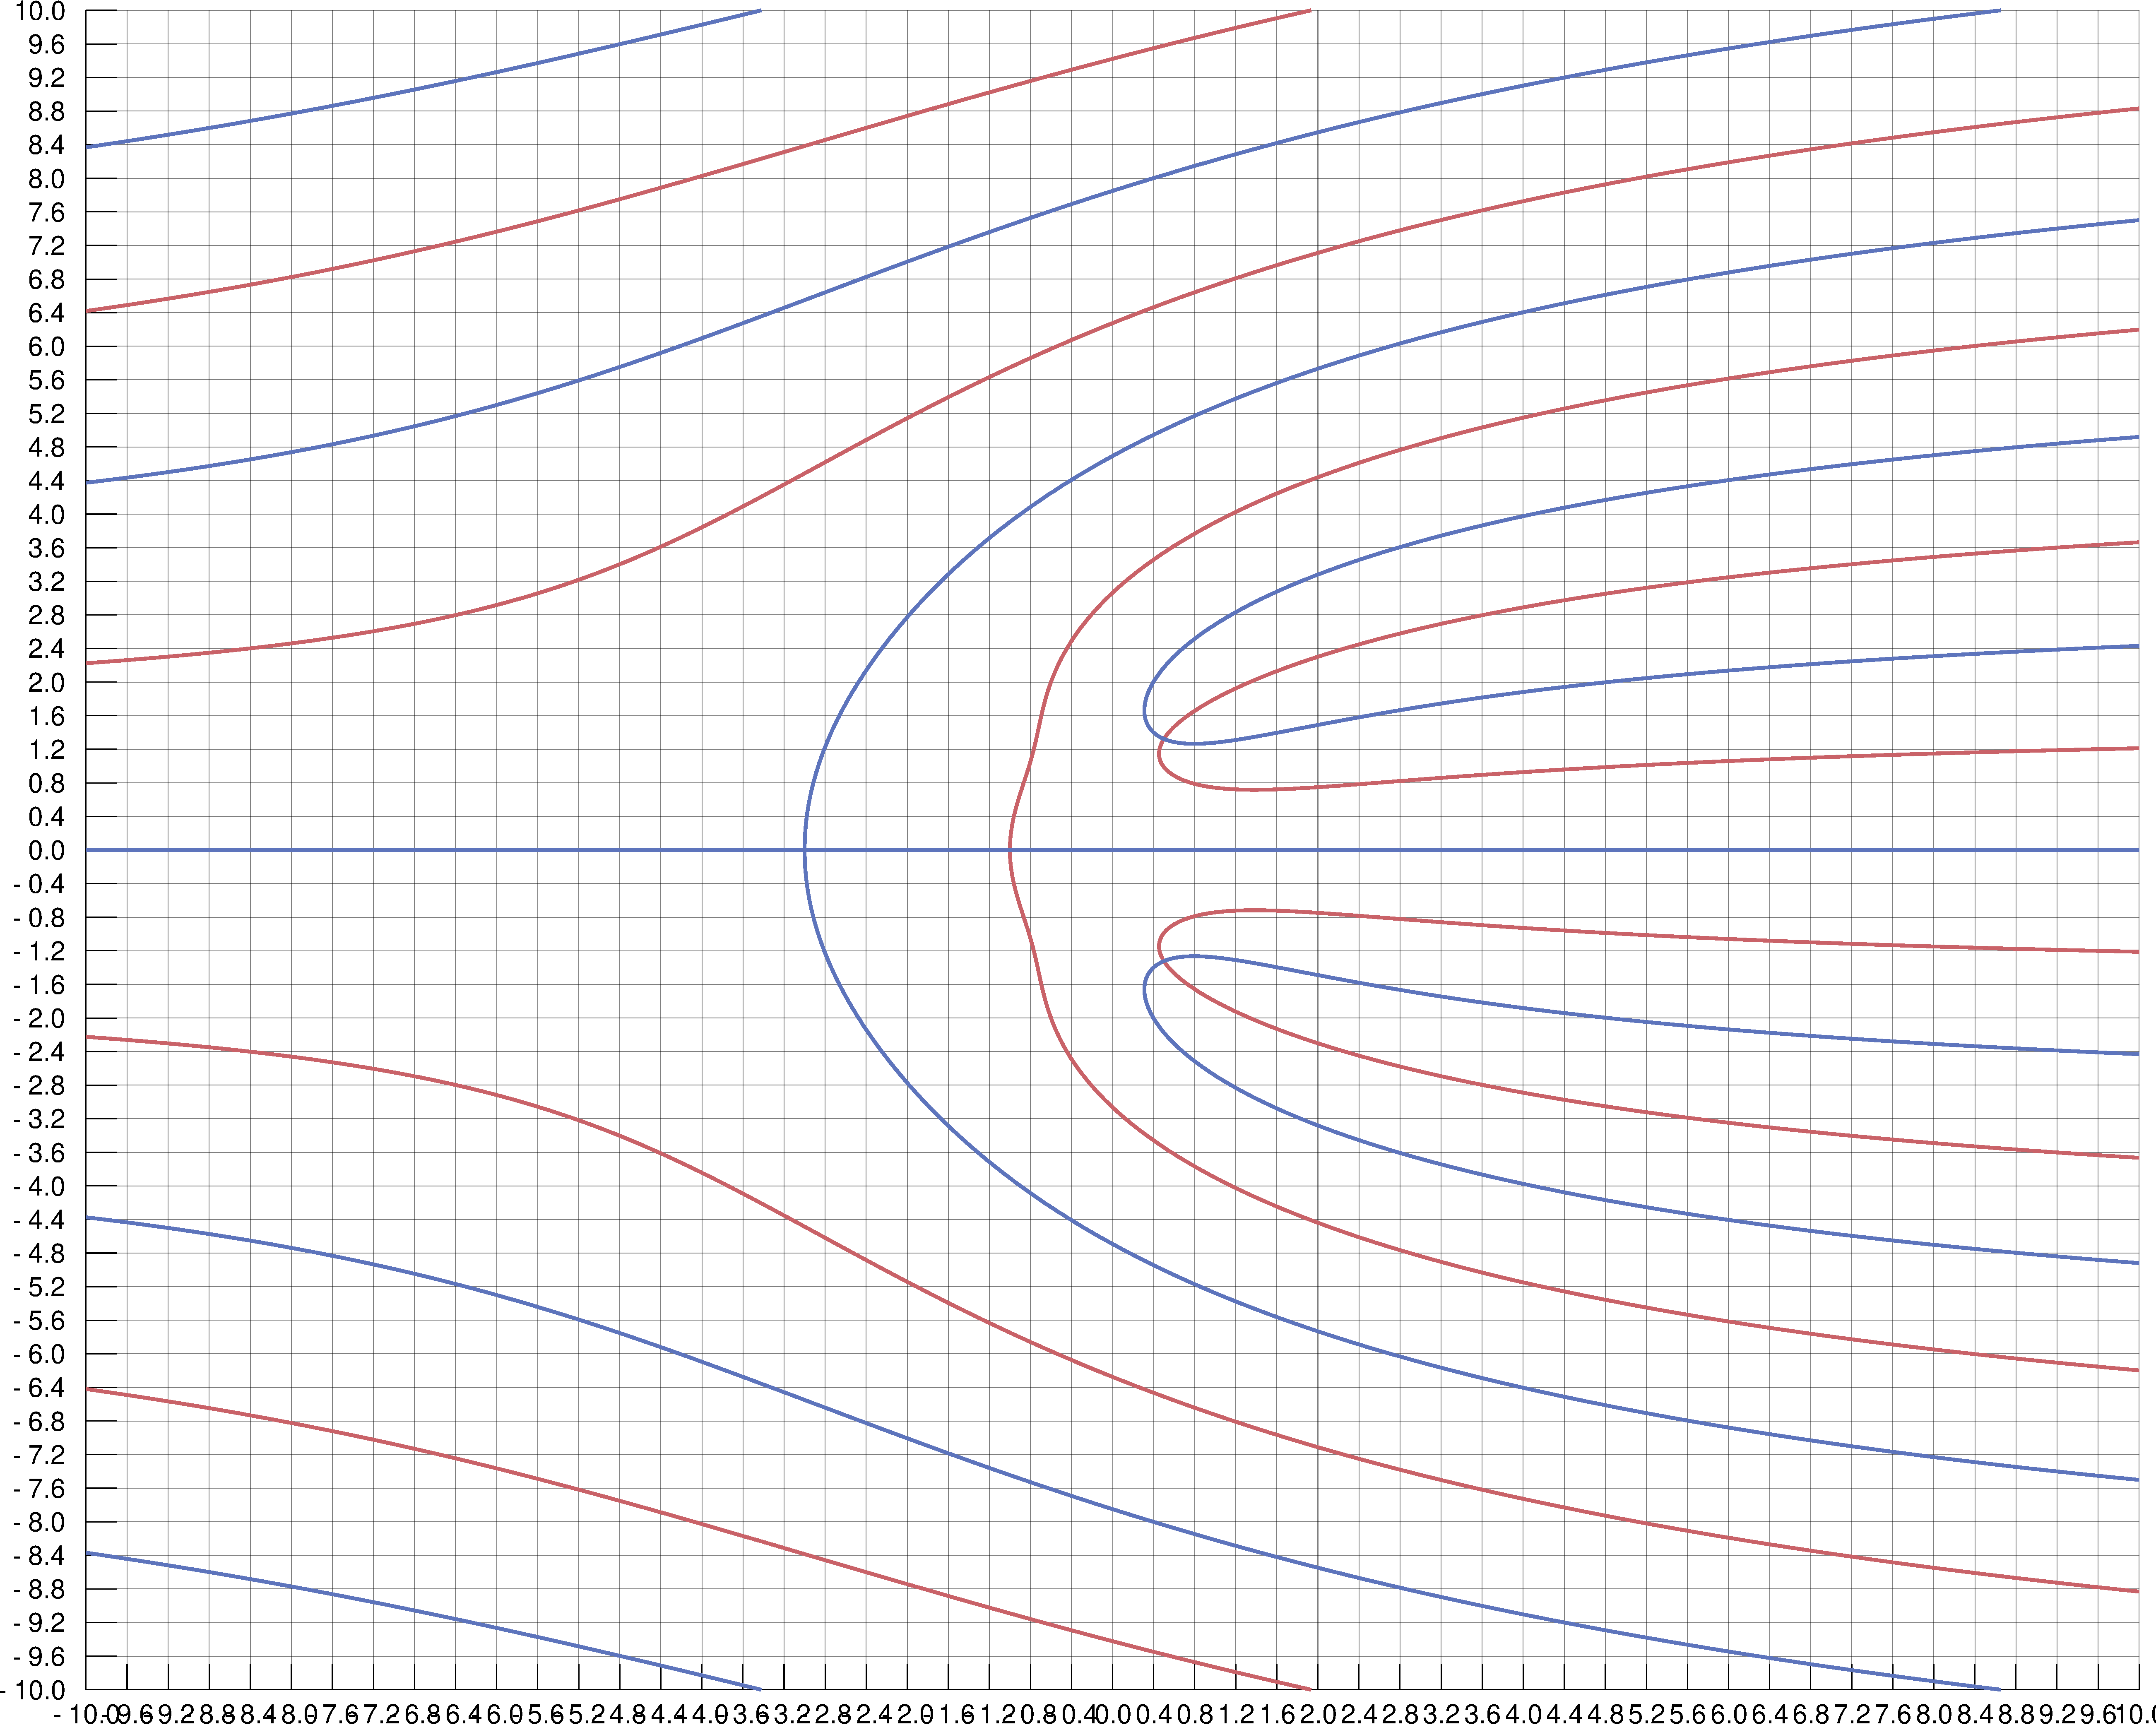
\includegraphics[width=1\linewidth]{levelCurves_3.pdf}
        \caption{$\Delta(\lambda) = (\lambda^3+\lambda+2)e^{\lambda}$.}
    \end{subfigure}
    \begin{subfigure}{.5\textwidth}
        \centering
        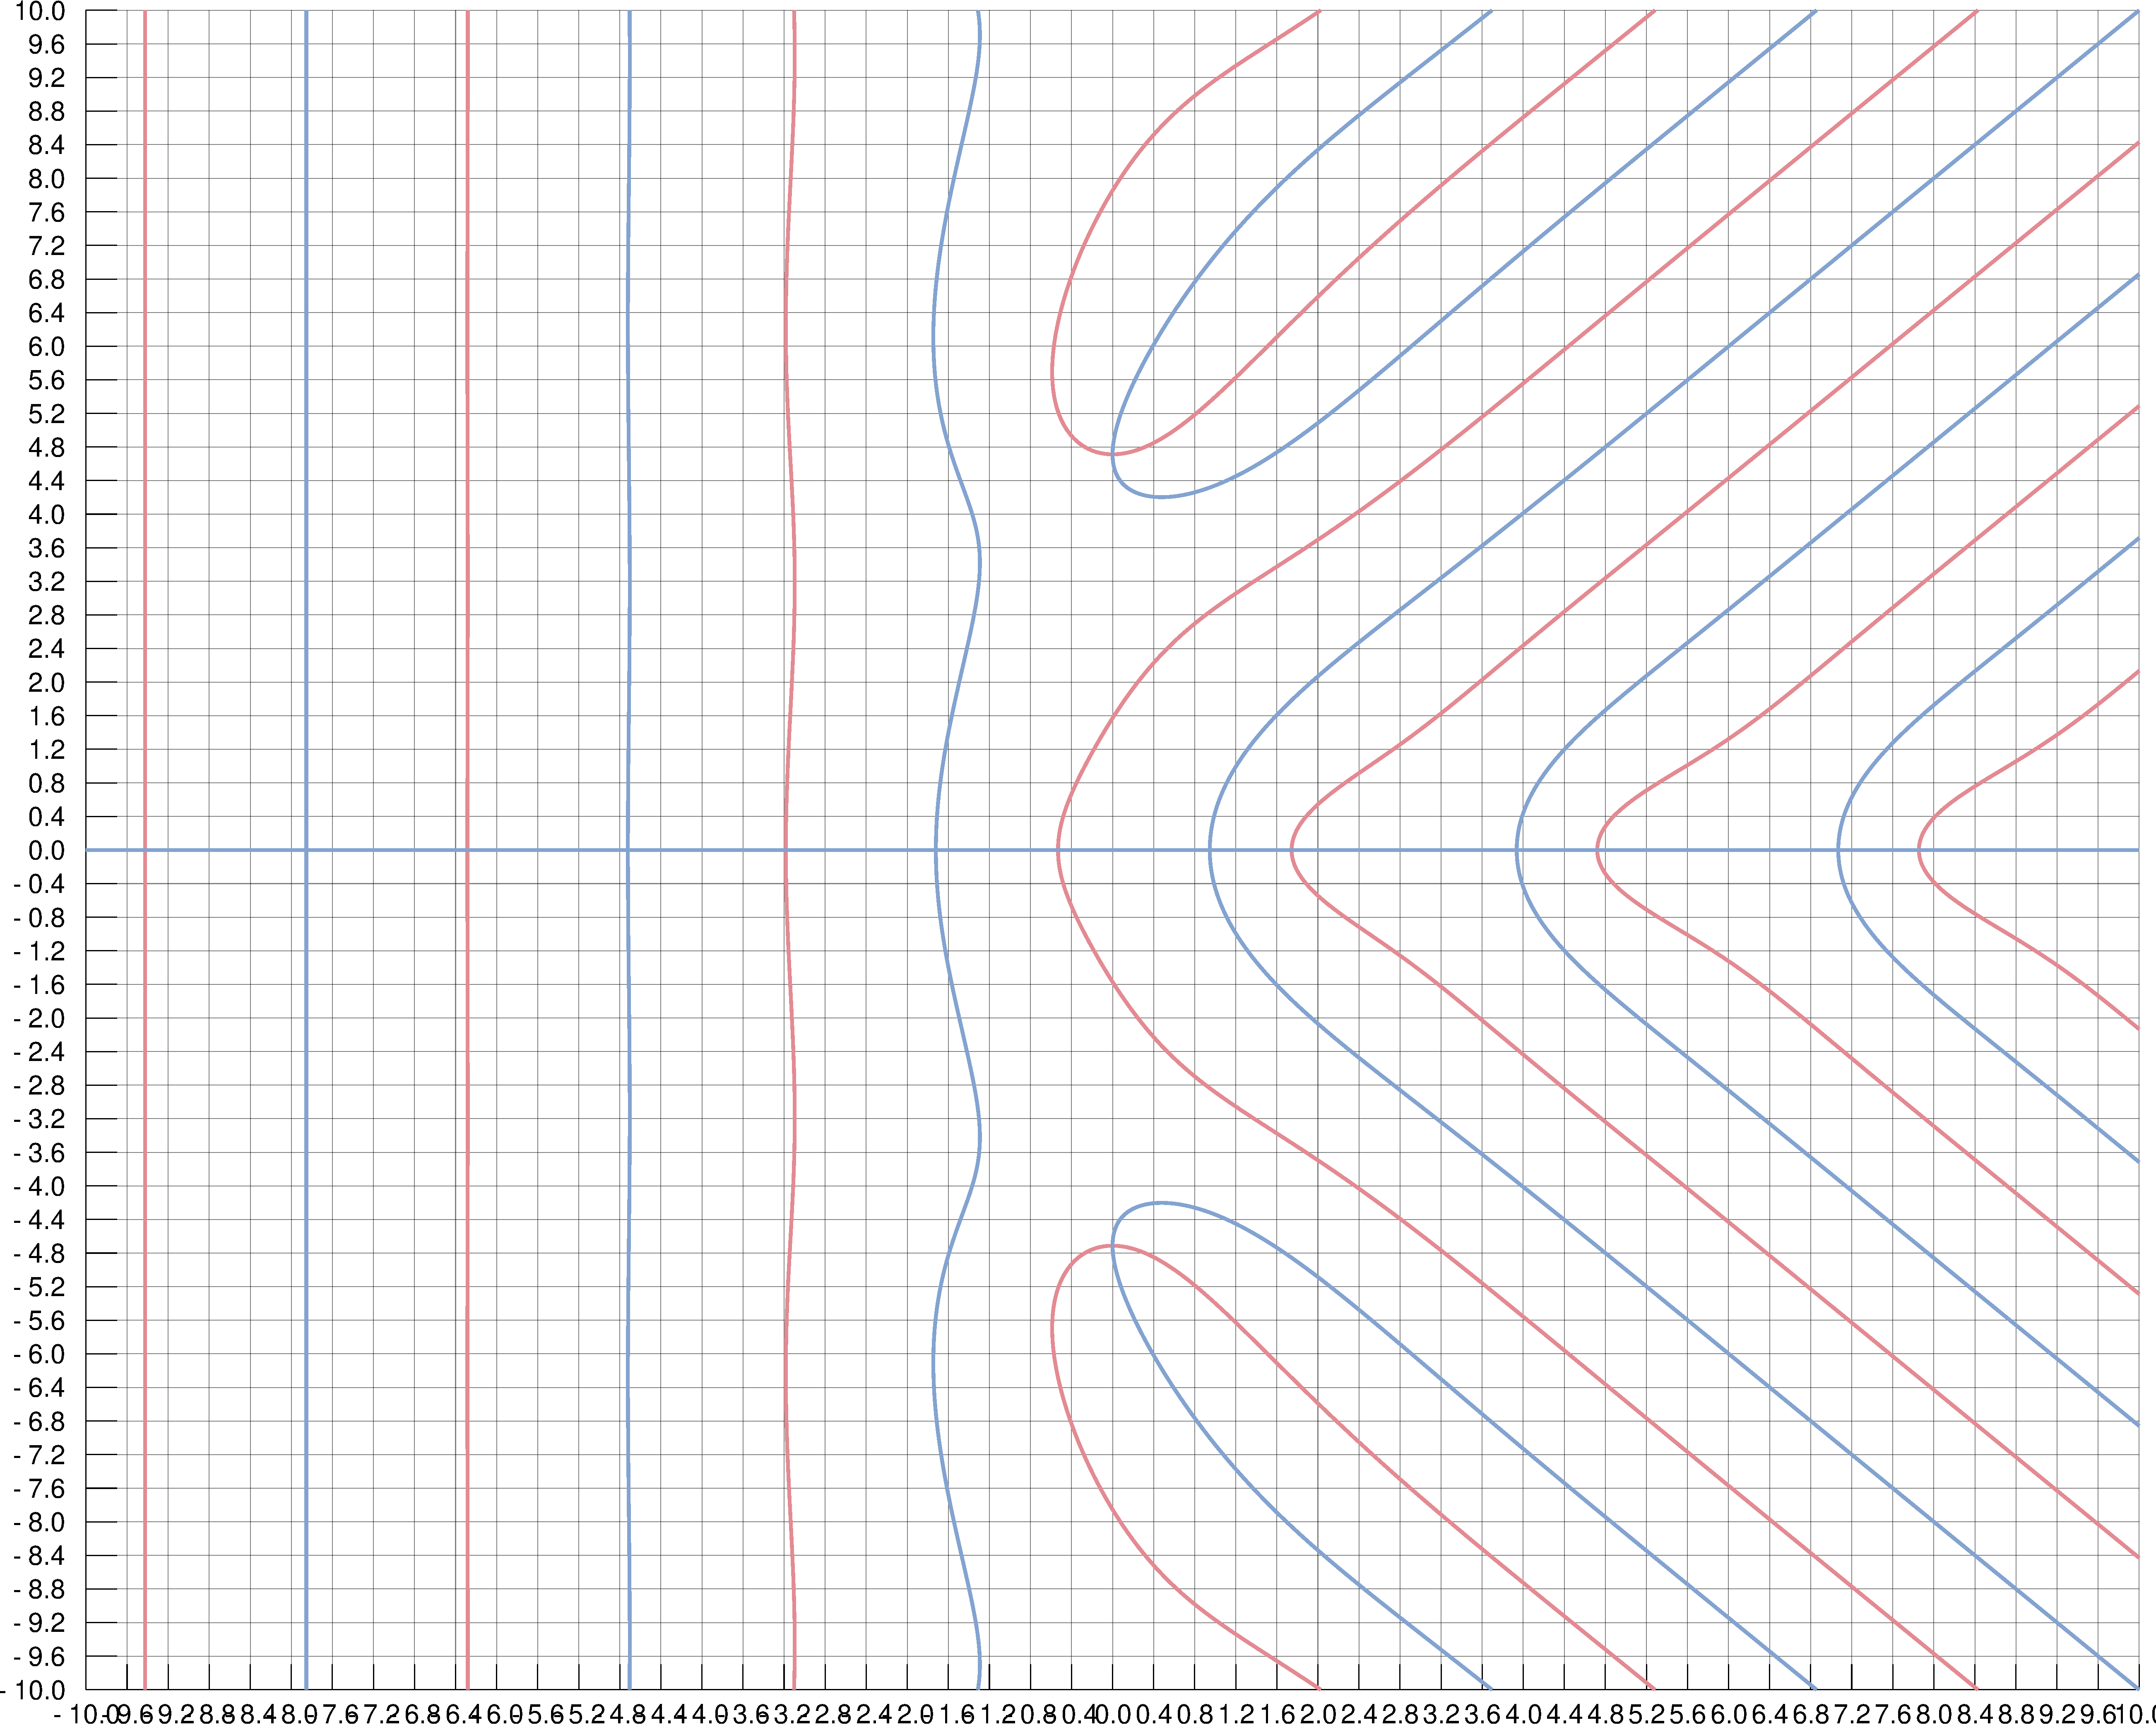
\includegraphics[width=1\linewidth]{levelCurves_4.pdf}
        \caption{$\Delta(\lambda) = \cos(\lambda)e^{\lambda} + \sin{\lambda}$.}
    \end{subfigure}
    \caption{Level curves corresponding to \eqref{eq:delta_real_imaginary}.}
    \label{fig:levelCurves}
\end{figure}

The above method still requires a human to read the level curve plots, visually locate the zeros of $\Delta(\lambda)$, and record them in an array, which can then be used as an input to the algorithm that produces $\Gamma$. Yet this does not introduce much inaccuracy: Recall that when constructing $\Gamma$, we need to deform the contours to avoid zeros of $\Delta(\lambda)$ with $N$-gons of radius $\epsilon$. Thus, there is relatively high tolerance for our approximation of the locations of the zeros.

\subsubsection{Constructing the integrands}\label{sec:constructing_integrands}

Having constructed the integration contours as above, theoretically, we can already compute the Fokas transform pair $F_\lambda$ and $f_x$ using equation \eqref{eq:fokas_transform_pair} and solve for $q(x,t)$ using equation \eqref{eq:q(x,t)_explicit}.
%Theoretically, the integrands $F^+_\lambda$ and $F^-_\lambda$ can be computed directly from \eqref{eq:F_lambda_+-}. 
Yet there is one more complication in practice. As shown in equation \eqref{eq:q(x,t)_explicit}, the solution $q(x,t)$ is a sum of integrals of $F_\lambda^+$, $F_\lambda^-$ over the contours $\Gamma$, but as shown in \eqref{eq:F+}--\eqref{eq:F-}, $F_\lambda^+$ and $F_\lambda^-$ themselves involve an integral of the initial datum $f(x)$. Double integrals are computationally expensive, and so to improve algorithm efficiency, we replace the inner integral involving $f(x)$ with an approximation of it that has explicit formula, developed as follows.

\paragraph{Approximating the inner integral using Chebyshev polynomials}\mbox{}\label{par:approximate_integral_chebyshev}

The inner integral in \eqref{eq:F_lambda_+-} that we wish to approximate is
\[\int_0^1 e^{-i\alpha^{l-1}\lambda x}f(x)\,dx,\]
where $f(x)$ is the initial datum of the IBVP in \eqref{eq:IBVP}.
Note that this is the Fourier transform of $f(x)$ on $[0,1]$ evaluated at $\alpha^{l-1}\lambda$.
The idea is to approximate $f(x)$ using Chebyshev polynomials and compute the integral using explicit formulas of the Fourier transform of Chebyshev polynomials \cite{Fokas2012}.

In this section, $n$ refers to the index of terms in the Chebyshev approximation of $f(x)$ instead of the spatial order of the IBVP in \eqref{eq:IBVP}.

The Chebyshev polynomials are given by
\[
    T_n(x) =
\begin{cases}
    \cos(n \arccos(x))&\quad\mbox{$|x|\leq 1$}\\
    \frac{1}{2}\left((x-\sqrt{x^2-1})^n + (x+\sqrt{x^2-1})^n\right)&\quad\mbox{$|x|>1$},
\end{cases}    
\]
for $n=0,1,2,\ldots$. Given a function $f_0(x)$ on the interval $[a,b]$, we can approximate $f_0(x)$ using Chebyshev polynomial expansion. The Chebyshev approximation is best on $[-1,1]$. Thus, we scale $[a,b]$ to $[-1,1]$ via $g:[a,b]\to [-1,1]$ given by $g(x)=2(x-a)/(b-a)-1$, obtain the Chebyshev coefficients $\{b_n\}_{n=0}^N$ there, and write the approximation of $f_0$ on $[a,b]$ as
\begin{equation}\label{eq:cheb_f_on_[a,b]}
    f_0(x)\approx \sum_{n=0}^N b_n T_n(g(x)),
\end{equation}
which is a finite sum of Chebyshev polynomials.

As shown in \eqref{eq:IBVP}, the IBVP's initial datum $f(x)$ is defined on $[0,1]$. Thus, we define $g(x):[0,1]\to [-1,1]$ by $g(x)=2x-1$. With the change of variable $t=g(x)=2x-1$, we have $x=g^{-1}(t)=\frac{t+1}{2}$. Let $h(t) := f\circ g^{-1}(t)$. Then $h(t)$ is defined on $[-1,1]$. Let $c:=\frac{\alpha^{l-1}\lambda}{2}$. Then
\begin{align*}
    \int_0^1 e^{-i\alpha^{l-1}\lambda x}f(x)\,dx &= \int_0^1 e^{-i2c\frac{t+1}{2}}f\left(\frac{t+1}{2}\right)\,d\left(\frac{t+1}{2}\right)\\
    &= \int_{-1}^1 e^{-ict}e^{-ic}f\left(\frac{t+1}{2}\right)\frac{1}{2}\,dt\\
    &= \frac{1}{2e^{ic}}\int_{-1}^1 e^{-ict} f\left(\frac{t+1}{2}\right)\,dt\\
    &= \frac{1}{2e^{ic}}\int_{-1}^1 e^{-ict} h(t)\,dt,
\end{align*}
Thus, it suffices to find 
\[\int_{-1}^1 e^{-ict} h(t)\,dt.\]

Suppose that on $[-1,1]$, the Chebyshev approximation of $h(t)$ is given by
\[h(t) \approx \sum_{n=0}^N b_n T_n(t).\]
Note that since $t=g(x)$, we have $f(x) = f(g^{-1}(g(x))) = h(g(x)) = h(t)$, and the above is equivalent to
\[f(x) \approx \sum_{n=0}^N b_n T_n(g(x)),\]
which is the same form as equation \eqref{eq:cheb_f_on_[a,b]}.
Thus, the Chebyshev coefficients of $h(t)$ are exactly the Chebyshev coefficients of $f(x)$ obtained on $[-1,1]$ after scaling. 

Since $t\in [-1,1]$, the Chebyshev polynomials $T_n(t)$ is given by $\cos(n\arccos(t))$, and thus
\[h(t) \approx \sum_{n=0}^N b_n \cos(n \arccos(t)).\]
Therefore,
\begin{align*}
    \int_{-1}^1 e^{-ict} h(t)\,dt &= \int_{-1}^1 e^{-ict} \sum_{n=0}^N b_n \cos(n \arccos(t))\,dt \\
    &= \sum_{n=0}^N b_n \int_{-1}^1 e^{-ict}\cos(n \arccos(t))\,dt.
\end{align*}
With the change of variable $t=\cos\theta$, we have
\begin{align*}
    \int_{-1}^1 e^{-ict}\cos(n \arccos(t))\,dt &= \int_{-1}^1 e^{-ic\cos\theta}\cos(n \arccos(\cos\theta))\,d\cos\theta\\
    &= \int_\pi^0 e^{-ic\cos\theta} \cos(n\theta) (-\sin\theta)\,d\theta\\
    &= \int_0^\pi e^{-ic\cos\theta} \cos(n\theta) \sin\theta\,d\theta.
\end{align*}

The remaining section presents material from \cite{Fokas2012} with proofs expanded.

Define
\begin{align*}
    \hat{T}_n(c) := \int_0^\pi e^{-ic\cos\theta} \cos(n\theta) \sin\theta\,d\theta.
\end{align*}
Then 
\begin{align*}
    \hat{T}_n(0) = \int_0^{\pi}\cos(n\theta)\sin\theta\,d\theta &=
    \begin{cases}
    2&\quad\mbox{if $n=0$}\\
    [\frac{1}{2}\sin^2\theta + \frac{0}{2}\cos^2\theta]_0^{\pi}&\quad\mbox{if $n=1$}\\
    \left[\frac{n}{n^2-1}\sin\theta\sin(n\theta) + \frac{1}{n^2-1}\cos\theta\cos(n\theta)\right]_0^{\pi}&\quad\mbox{if $n\geq 2$}
    \end{cases}\\
    &= 
    \begin{cases}
    2&\quad\mbox{if $n=0$}\\
    \frac{1}{2}\sin^2(\pi) - \frac{1}{2}\sin^2(0)&\quad\mbox{if $n=1$}\\
    \frac{n}{n^2-1}\sin(\pi)\sin(n\pi) + \frac{1}{n^2-1}\cos(\pi)\cos(n\pi)\\ 
    \qquad - \frac{n}{n^2-1}\sin(0)\sin(0) - \frac{1}{n^2-1}\cos(0)\cos(0)&\quad\mbox{if $n\geq 2$}
    \end{cases}\\
    &= 
    \begin{cases}
    2&\quad\mbox{if $n=0$},\\
    0&\quad\mbox{if $n=1$},\\
    \frac{(-1)^{n+1}-1}{n^2-1}&\quad\mbox{if $n\geq 2$}.
    \end{cases}
\end{align*}
Note that the formula for $n\geq 2$ agrees with the case for $n=0$, but for clarity, we write them separately.
For $c\in\C\setminus\{0\}$, using integration by parts, we have
\begin{align*}
    \hat{T}_n(c) &= \int_0^\pi e^{-ic\cos\theta}\cos(n\theta)\sin\theta\,d\theta\\
    &= \left[\cos(n\theta)\frac{1}{ic}e^{-ic\cos\theta}\right]_0^{\pi} - \int_0^{\pi}\frac{1}{ic}e^{-ic\cos\theta}n(-\sin(n\theta))\,d\theta\\
    &= \left[\cos(n\pi)\frac{1}{ic}e^{-ic\cos(\pi)} - \cos(0)\frac{1}{ic}e^{-ic\cos 0}\right] + \frac{n}{ic}\int_0^{\pi}e^{-ic\cos\theta}\sin(n\theta)\,d\theta\\
    &= \frac{1}{ic}\left(n\int_0^{\pi}e^{-ic\cos\theta}\sin(n\theta)\,d\theta + (-1)^n e^{ic}- e^{-ic}\right).
\end{align*}

Let $z\in \C\setminus\{0\}$, define 
\[K_n(z):=\int_0^\pi e^{z\cos\theta}\sin(n\theta)\,d\theta.\]
Then for $c\in\mathbb{C}\setminus\{0\}$,
\begin{align*}
\hat{T}_n(c) &= \frac{1}{ic}\left(n\int_0^{\pi}e^{-ic\cos\theta}\sin(n\theta)\,d\theta + (-1)^n e^{ic}- e^{-ic}\right)\\
&= \frac{1}{ic}\left(nK_n(-ic) + (-1)^n e^{ic} - e^{-ic}\right).
\end{align*}
We note that
\begin{align*}
K_0(z) &= \int_0^{\pi}e^{z\cos\theta}\sin 0\,d\theta=0\\
K_1(z) &= \int_0^{\pi}e^{z\cos\theta}\sin\theta\,d\theta\\
&= \left[-\frac{1}{z}e^{z\cos\theta}\right]_0^{\pi}\\
&= -\frac{1}{z}e^{z\cos(\pi)} + \frac{1}{z}e^{z\cos 0}\\
&= \frac{e^z - e^{-z}}{z}.
\end{align*}
To compute $K_n(z)$ for $n\geq 2$, we first note that
\begin{align*}
\sin((n+1)\theta) - \sin((n-1)\theta) &= \frac{e^{i(n+1)\theta} - e^{-i(n+1)\theta}}{2i} - \frac{e^{i(n-1)\theta} - e^{-i(n-1)\theta}}{2i}\\
&= \frac{e^{in\theta}e^{i\theta} - e^{in\theta}e^{-\theta} - e^{-in\theta}e^{-i\theta} + e^{-in\theta}e^{i\theta}}{2i}\\
&= \frac{(e^{i\theta}-e^{-i\theta})(e^{in\theta}+e^{-in\theta})}{2i}\\
&= 2\left(\frac{e^{i\theta}-e^{-i\theta}}{2i}\right)\left(\frac{e^{in\theta}+e^{-in\theta}}{2}\right)\\
&= 2\sin\theta\cos(n\theta).
\end{align*}
So
$$\sin((n+1)\theta) = \sin((n-1)\theta) + 2\sin\theta\cos(n\theta).$$
Thus,
\begin{align*}
K_{n+1}(z) &= \int_0^{\pi}e^{z\cos\theta}\sin((n+1)\theta)\,d\theta\\
&= \int_0^{\pi}e^{z\cos\theta}(\sin((n-1)\theta) + 2\sin\theta\cos(n\theta))\,d\theta\\
&= \int_0^{\pi}e^{z\cos\theta}\sin((n-1)\theta)\,d\theta + 2\int_0^{\frac{\pi}{2}}e^{z\cos\theta}\sin\theta\cos(n\theta)\,d\theta\\
&= K_{n-1}(z) + 2\int_0^{\pi}\cos(n\theta)\sin\theta e^{z\cos\theta}\,d\theta.
\end{align*}
Using integration by parts,
\begin{align*}
\int_0^{\pi}\cos(n\theta)\sin\theta e^{z\cos\theta}\,d\theta &= \left[-\frac{1}{z}e^{z\cos\theta}\cos(n\theta)\right]_0^{\pi} - \int_0^{\pi}\frac{1}{z}e^{z\cos\theta}n\sin(n\theta)\,d\theta\\
&= -\frac{1}{z}e^{z\cos(\pi)}\cos(n\pi) + \frac{1}{z}e^{z\cos 0}\cos 0 - \frac{n}{z}\int_0^{\pi}e^{z\cos\theta}\sin(n\theta)\,d\theta\\
&= \frac{e^z}{z} + (-1)^{n+1}\frac{e^{-z}}{z} - \frac{n}{z}K_n(z).
\end{align*}
Thus, $K_n(z)$ satisfies the recurrence relation
\begin{align*}
K_0(z) &= 0\\
K_1(z) &= \frac{e^z-e^{-z}}{z}\\
K_{n}(z) &= K_{n-2}(z) + 2\left(\frac{e^z}{z} + (-1)^{n}\frac{e^{-z}}{z} - \frac{n-1}{z}K_{n-1}(z)\right),\quad n\geq 2.
\end{align*}
Further solving the recurrence relation \cite{Fokas2012} gives
\begin{alignat*}{2}
    \hat{T}_n(c) = \int_0^\pi e^{-ic\cos\theta}\cos(n\theta)\sin\theta\,d\theta &= 
    \begin{cases}
        2 &\quad\mbox{if $n=0$},\\
        0 &\quad\mbox{if $n=1$},\\
        \frac{(-1)^{n+1}-1}{n^2-1} &\quad\mbox{if $n\geq 2$},
    \end{cases}
    &\quad\mbox{if $c=0$},\\
    &= \sum_{m=1}^{n+1}\alpha(m,n)\left[\frac{e^{i\lambda}}{(i\lambda)^m} + (-1)^{m+n}\frac{e^{-i\lambda}}{(i\lambda)^m}\right]&\quad\mbox{if $c\neq 0$},
\end{alignat*}
where
\begin{align*}
\alpha(m,n) =
\begin{cases}
(-1)^n&\quad\mbox{if $m=1$},\\
(-1)^{n+1}n^2&\quad\mbox{if $m=2$},\\
(-1)^{n+m-1}2^{m-2}n\sum_{k=1}^{n-m+2}\binom{m+k-3}{k-1}\prod_{j=k}^{m+k-3}(n-j)&\quad\mbox{if $m=3,4,\ldots,n+1$}.
\end{cases}
\end{align*}

Thus, in summary,
\begin{align*}
    \int_0^1 e^{-i\alpha^{l-1}\lambda x}f(x)\,dx &= \frac{1}{2e^{ic}}\int_{-1}^1 e^{-ict} h(t)\,dt\\
    &\approx \frac{1}{2e^{ic}}\sum_{n=0}^N b_n \int_{-1}^1 e^{-ict}\cos(n \arccos(t))\,dt\\
    &= \frac{1}{2e^{ic}}\sum_{n=0}^N b_n \hat{T}_n(t),
\end{align*}
with $\hat{T}_n(t)$ given above.

\section{Implementation}
\subsection{Overview}
The above algorithm is implemented in Julia 0.6.4. Library dependencies are \texttt{SymPy} \cite{sympy}, \texttt{sympy} \cite{sympyPython},  \texttt{Distributions} \cite{distributions}, \texttt{ApproxFun} \cite{approxfun}, \texttt{Roots} \cite{roots}, \texttt{QuadGK} \cite{quadgk}, \texttt{Plots} \cite{plots}, \texttt{Gadfly} \cite{gadfly}, and \texttt{PyPlot} \cite{pyplot}. Code, unit tests, and documentation with examples can be found in \cite{Xiao}, with possibly minor differences in notation from section \ref{sec:fokas_transform_pair}.

As mentioned near the end of section \ref{sec:motivation}, the implementation aims at providing computer aid alongside human judgment in the process of using the Fokas method to solve IBVPs.

\subsection{Sample usage}
We illustrate the utilities of the implementation using two cases of sample usage below. More details can be found in the documentation \cite{Xiao}.

\subsubsection{Solving IBVP}\label{sec:ex1}
In this section, we show how the implementation provides computer aid in the process of applying the Fokas method.

Consider the heat equation IBVP
\begin{subequations}\label{eq:ex1}
    \begin{alignat}{3}
        q_t - q_{xx} &= 0\quad &\forall (x,t)&\in (0,1)\times (0,T) \label{eq:ex1_PDE}\\
        q(x,0) &= f(x) \quad &\forall x&\in [0,1]\label{eq:ex1_initial_condition}\\
        q(0,t) - q(1,t) &= 0 &\forall t&\in [0,T]\label{eq:ex1_boundary_condition1}\\
        q_x(0,t) - q_x(1,t) &= 0 &\forall t&\in [0,T]\label{eq:ex1_boundary_condition2},
    \end{alignat}
\end{subequations}
where $f(x)$ also satisfies equations \eqref{eq:ex1_boundary_condition1}--\eqref{eq:ex1_boundary_condition2}.

Rewriting the IBVP in the form \eqref{eq:IBVP}, we have $n=2$, $a=1$,
\[S= (-i)^2 \frac{d^2}{dx^2} = -\frac{d^2}{dx^2},\]
\begin{align*}
B_1\phi &= 1\cdot \varphi(0) + (-1)\cdot \varphi(1) + 0\cdot \varphi^{(1)}(0) + 0\cdot \varphi^{(1)}(1)\\
B_2\phi &= 0\cdot \varphi(0) + 0\cdot \varphi(1) + 1\cdot \varphi^{(1)}(0) + (-1)\cdot \varphi^{(1)}(1),
\end{align*}
and
\[\Phi = \{\phi\in C^{\infty}[0,1]:\, B_j\phi = 0\,\forall j\in\{1,2\}\}.\]
Using the notation in section \ref{sec:construct_adjoint}, the two matrices associated with the vector boundary form corresponding to the above boundary conditions are
$$M = \begin{bmatrix}1&0\\0&1\end{bmatrix},\quad N = \begin{bmatrix}-1&0\\0& -1 \end{bmatrix}.$$
We choose $f(x)=\sin(2\pi x)$ to be the initial datum. Then $f(x)$ satisfies
\begin{align*}
Uf = \begin{bmatrix}
1&0& -1 &0\\
0&1&0& -1
\end{bmatrix} \begin{bmatrix}f(0)\\f'(0)\\f(1)\\f'(1)\end{bmatrix} = 0.
\end{align*}
By \eqref{eq:Ux=Mxi(a)+Nxi(b)}, $f\in \Phi$, as required.

The adjoint vector boundary form found by the algorithm outlined in section \ref{sec:construct_adjoint} is characterized by the matrices
% \begin{subequations}\label{eq:ex1_b_beta}
% \begin{align}
%     b^\star &= \begin{bmatrix}0&-1\\ 1&0\end{bmatrix},\\
%     \beta^\star &= \begin{bmatrix}0&1\\ -1&0\end{bmatrix}.
% \end{align}
% \end{subequations}
\begin{equation}\label{eq:ex1_b_beta}
    b^\star = \begin{bmatrix}0&-1\\ 1&0\end{bmatrix}, \quad \beta^\star = \begin{bmatrix}0&1\\ -1&0\end{bmatrix}.
\end{equation}
From \eqref{eq:ex1_b_beta}, we compute $\Delta(\lambda)$ in \eqref{eq:delta} to be 
\begin{equation}\label{eq:ex1_delta}
    \Delta(\lambda) = 8i\lambda \sin^2\left(\frac{\lambda}{2}\right),
\end{equation}
and $F_\lambda^+(f)$, $F_\lambda^-(f)$ in \eqref{eq:F_lambda_+-} to be
\begin{subequations}\label{eq:ex1_F_lambda_+-}
    \begin{align}
        F_\lambda^+(f) &= \frac{\hat{f}(\lambda)e^{i\lambda}}{2\pi(e^{i\lambda}-1)}\\
    F_\lambda^-(f) &= \frac{\hat{f}(\lambda)}{2\pi(e^{i\lambda}-1)},
    \end{align}
\end{subequations}
where 
%$\alpha = e^{2\pi i/n}$ and 
$\hat{f}(\lambda)=\int_0^1 e^{i\lambda x}f(x)\,dx$ is approximated using the method in section \ref{par:approximate_integral_chebyshev}.

From the level curves corresponding to \eqref{eq:delta_real_imaginary} in Figure \ref{fig:ex1_levelCurves}, we see that the zeros of $\Delta(\lambda)$ are $-2\pi, 0, 2\pi$ (with the modulus of complex infinity $d$ set as $10$).
\begin{figure}[htpb!]
    \centering
    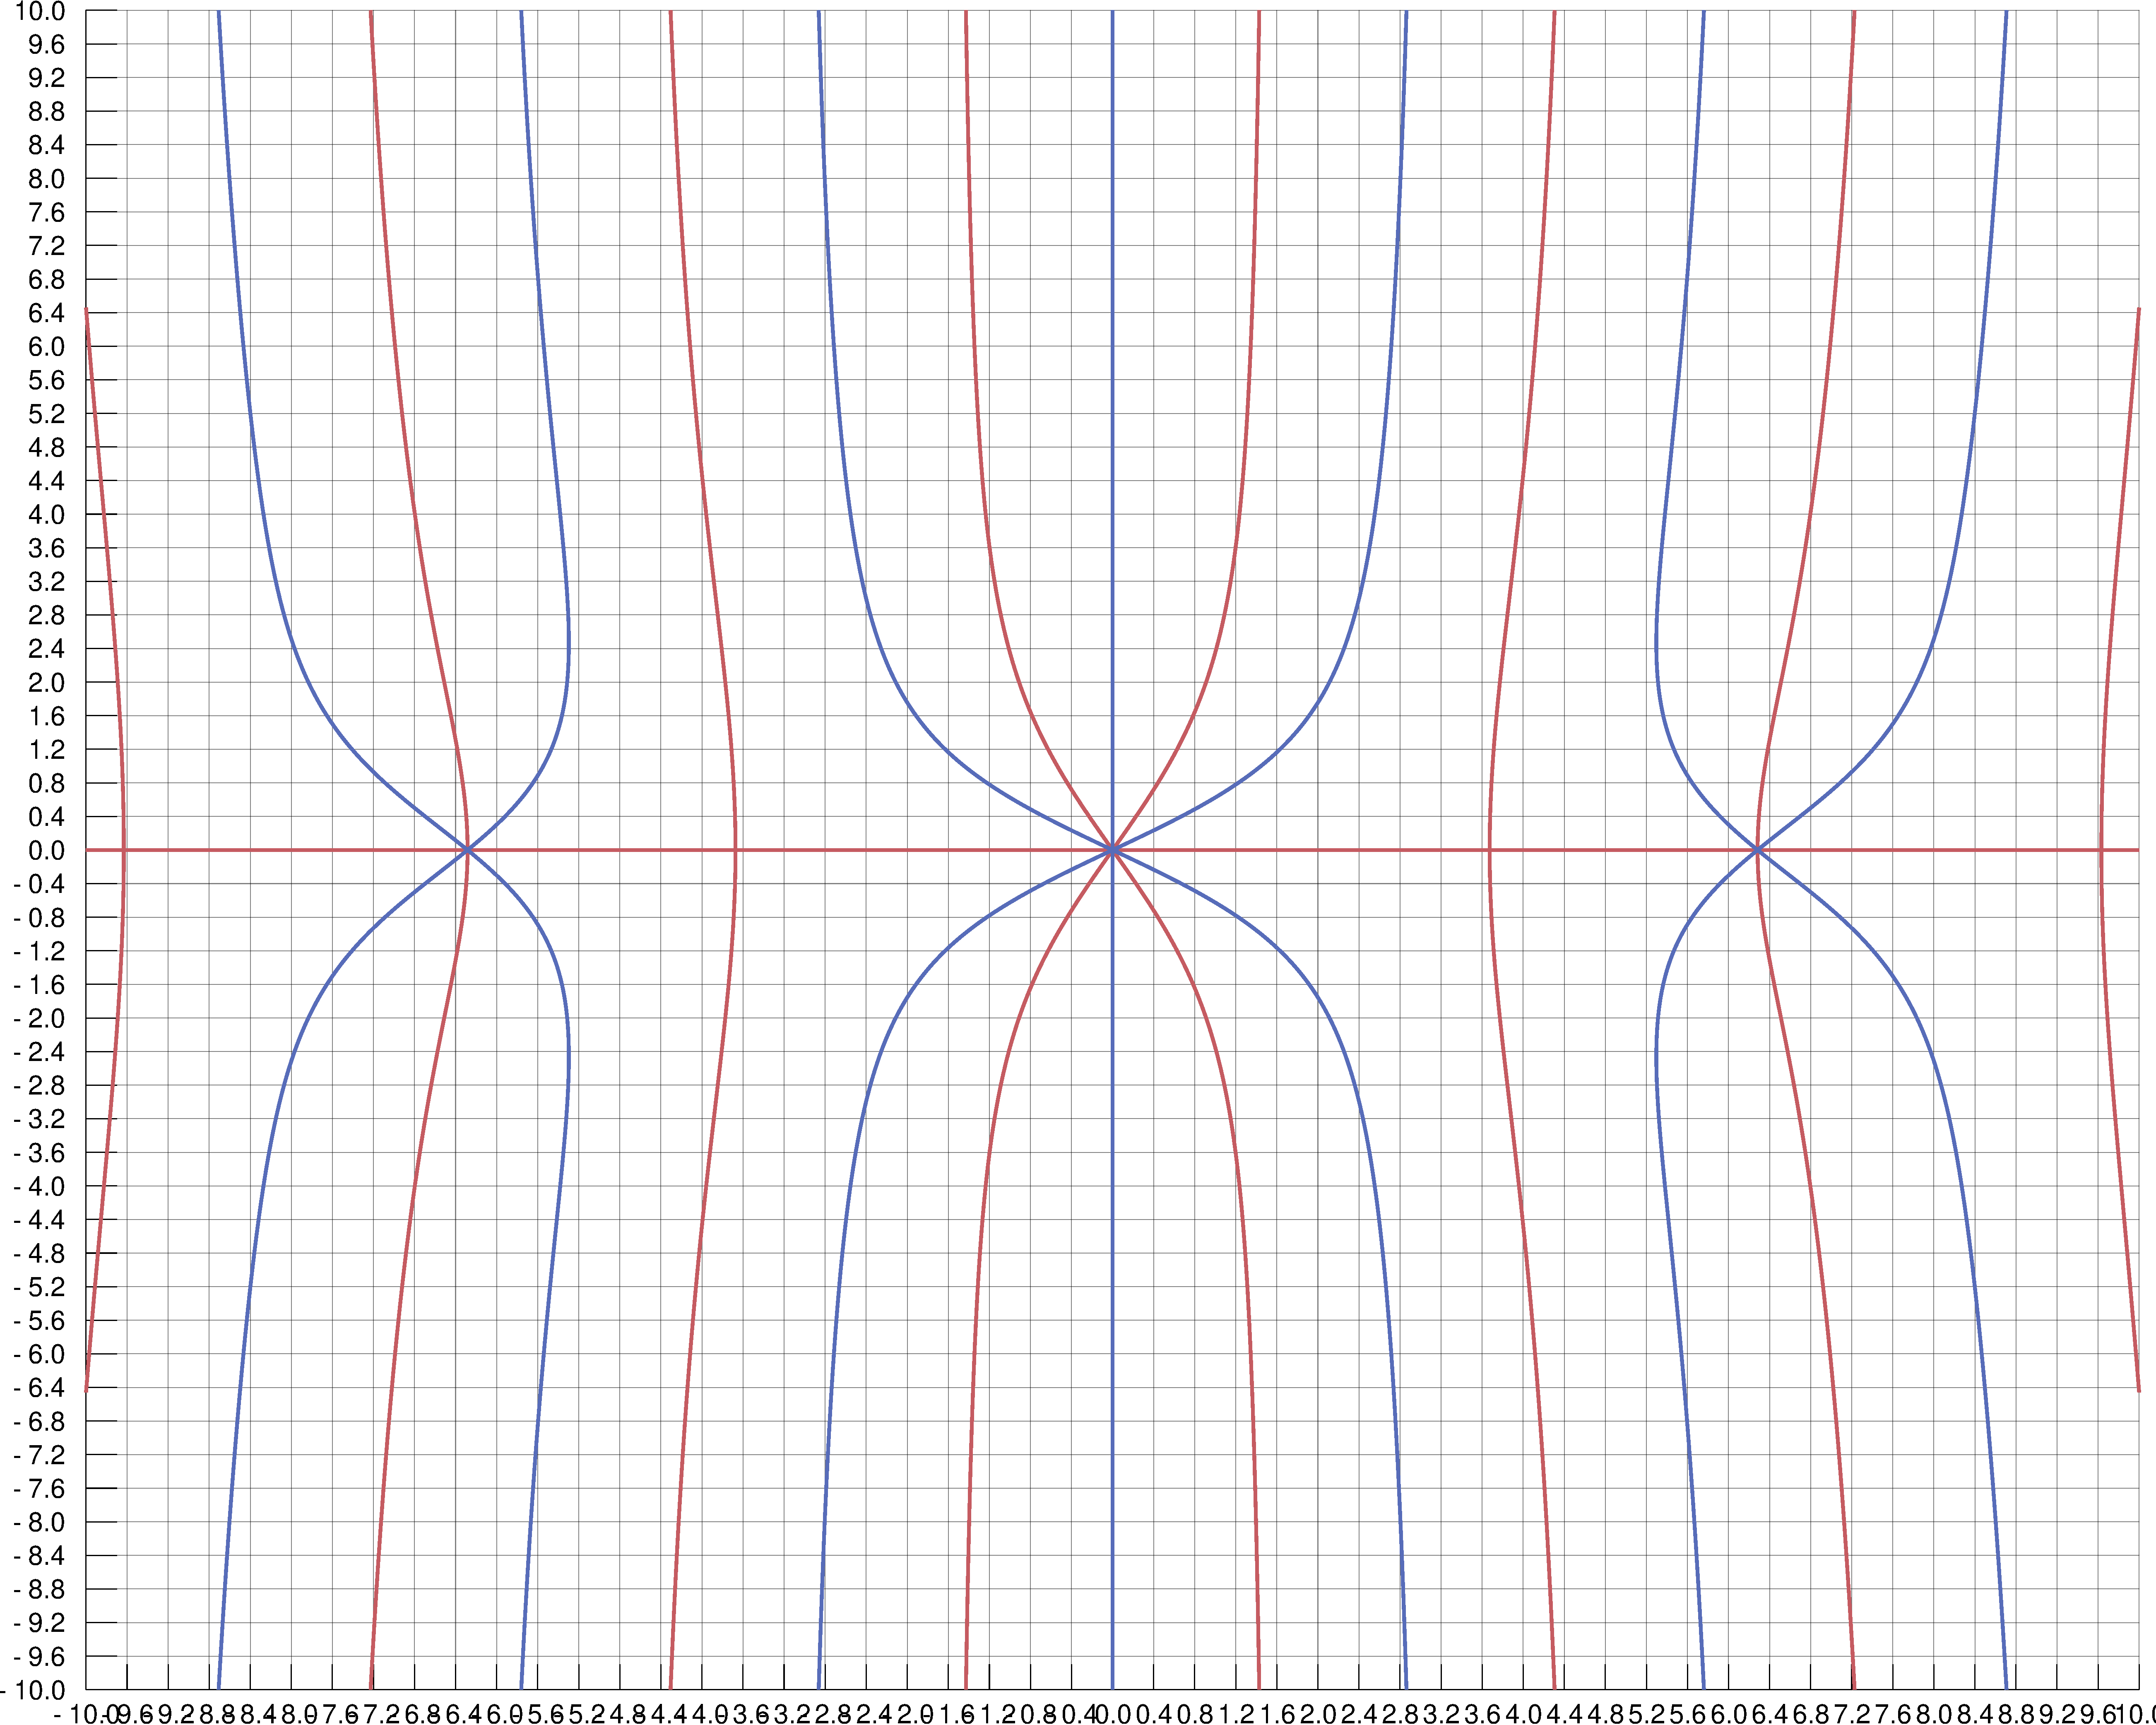
\includegraphics[width=1\linewidth]{ex1_levelCurves.pdf}
    \caption{Level curves corresponding to \eqref{eq:delta_real_imaginary} with $\Delta(\lambda)$ defined in \eqref{eq:ex1_delta}.}
    \label{fig:ex1_levelCurves}
\end{figure}
With this information, we find the contours $\Gamma$ to be as in Figure \ref{fig:ex1_contourPlot}.
\begin{figure}[htpb!]
    \centering
    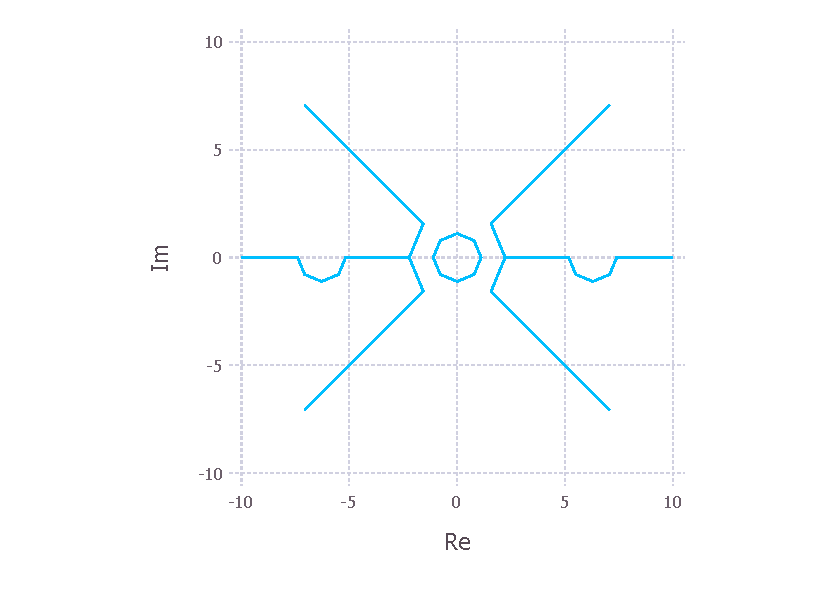
\includegraphics[width=1\linewidth]{ex1_contourPlot.pdf}
    \caption{The $\Gamma$ contour.}
    \label{fig:ex1_contourPlot}
\end{figure}

As shown in equation \eqref{eq:q(x,t)_explicit}, to compute $q(x,t)$, we need to evaluate $e^{i\lambda x}e^{-a\lambda^n t}F_\lambda^\pm(f)$ over the contours $\Gamma_a^\pm$ and $\Gamma_0^\pm$, respectively; call this the outer integral. We note that the inner integral $\int_0^1 e^{i\alpha^{l-1}\lambda x}f(x)\,dx$ in \eqref{eq:F_lambda_+-} depends on both $\lambda$ and $f$. One consequence of this is that if $F_\lambda^+$, $F_\lambda^-$ are to be implemented as functions without symbolic expressions, they each need to take both $\lambda$ and $f$ as arguments. But doing so results in unnecessary computational cost: The outer integral is over $\lambda$ only, meaning that, when evaluating it, $\lambda$ changes while $f$ does not. But once $\lambda$ changes, the inner integral also needs to be re-calculated, and because it depends on $f$ and $\lambda$, the procedure to approximate the integral described in section \ref{par:approximate_integral_chebyshev} would need to be repeated. As a result, when evaluating $q(x,t)$, the Chebyshev approximation of $f$ is re-calculated at each point in the $\Gamma$ contour even though $f$ does not change throughout the process. Current implementation of the Fokas method in this project avoids such unnecessary computational cost by computing the explicit symbolic formulas of $F_\lambda^+$, $F_\lambda^-$ that depend on $\lambda$ only; these symbolic formulas are derived by replacing $\hat{f}(\lambda)$ in \eqref{eq:ex1_F_lambda_+-} with the symbolic expression of the approximation of $\int_0^1 e^{i\lambda x}f(x)\,dx$ obtained in section \ref{par:approximate_integral_chebyshev}.
%these formulas are obtained from \eqref{eq:ex1_F_lambda_+-}, with $\hat{f}(\lambda)$ replaced by the approximation of $\int_0^1 e^{i\lambda x}f(x)\,dx$ obtained in section \ref{par:approximate_integral_chebyshev}, written as a symbolic expression in $\lambda$. 
In this way, components of the outer integral that depend on $f$ are evaluated only once.
%This is also the only way to avoid the cost.

In practice, we would convert the symbolic formulas into function objects, because in Julia, function objects are evaluated much faster than symbolic objects. More recent versions of Julia have parsers that perform the conversion. In Julia 0.6.4 in which the current implementation is based (for reasons explained in the last paragraph in section \ref{sec:motivation}), however, no such parser exists, and conversion needs to be done manually, namely to create the corresponding function objects by typing in the symbolic formulas in the function definition. Having done so, current implementation of the Fokas method in this project allows evaluating $q(x,t)$ at a given $(x_0, t_0)\in (0,1)\times (0,T)$ within $20$ seconds with the modulus of complex infinity set as $10$, and within $1$ minute with the modulus of complex infinity set as $50$ (which is a more reasonable value regarding numerical accuracy, as explained in section \ref{sec:deform_contours}).

As a side note, the solution $q(x,t)$ computed above using equation \eqref{eq:q(x,t)_explicit} corresponds to the separated solution of the heat equation \cite{Pinsky1991} in the following sense. Using Cauchy's theorem and Jordan's lemma from complex analysis, it can be shown that integration over the $\Gamma$ contour in Figure \ref{fig:ex1_contourPlot} reduces to integration over closed contours around the poles of $F^+_\lambda$ and $F^-_\lambda$, i.e., the zeros of $\Delta(\lambda)$ in Figure \ref{fig:ex1_levelCurves}. That is, $q(x,t)$ reduces to a sum of contour integrals around zeros of $\Delta(\lambda)$, and using the residue theorem, these contour integrals can be shown to correspond to the eigenfunctions of Sturm-Liouville BVP related to the heat equation IBVP. Since $\Delta(\lambda)$ have infinitely many zeros on the real line, as the estimate of the modulus of complex infinity $d$ tends to $\infty$, $\Gamma$ would effectively consist of infinitely many closed contours centered on the real line (much like the blue circles on $\real(\lambda)$ in Figure \ref{fig:gamma_smith_fokas}, but extending to $\infty$ in both directions). As a result, $q(x,t)$ would become an infinite series of contour integrals, which is none other than the separated solution of the heat equation of the form 
\[q(x,t) = \sum_{n=1}^\infty A_n \phi_n(x)e^{-\lambda_n Kt},\]
where $A_n$ are Fourier coefficients of the initial datum $f(x)$, $\lambda_n$ the eigenvalues of the Sturm-Liouville problem, and $\phi_n(x)$ the corresponding eigenfunctions. Such correspondence to the separated solution is no surprise since the Fokas transform method originated from a deeper form of separation of variables \cite{Fokas1997}\cite{Fokas2009}. This is also reflected in the fact that methods based on transform pairs essentially separate the spatial and temporal components of the IBVP.

\subsubsection{Symbolic computation}\label{sec:symbolic_computation}

In this section, we illustrate how the symbolic computation feature of the implementation can be useful.

Applying the Fokas method to IBVPs and beyond depends on two technical lemmas, one concerning the positions of the poles of $F^+_\lambda$, $F^-_\lambda$ (i.e., zeros of $\Delta(\lambda)$), the other concerning the asymptotic decay of $F^+_\lambda$, $F^-_\lambda$. These lemmas are first described in \cite{Smith2012} for IBVPs. Their precise roles are more clearly articulated in \cite{Miller2018}, which also describes the extension of the Fokas method to a broader class of problems. These lemmas may assume variations for different types of problems such as those described in the beginning of section \ref{sec:discussion}, but some version of them are always required when applying the Fokas method. Because of the way these lemmas make statements about $F^+_\lambda$ and $F^-_\lambda$, in proving them or their variations, it would be helpful to have the symbolic formulas for $F^+_\lambda$, $F^-_\lambda$.

For the IBVPs \eqref{eq:problem_1} and \eqref{eq:problem_2}, the formulas for $F_\lambda^+$ and $F_\lambda^-$ have been computed by hand in \cite[p. 1-4]{Smith2016}. Symbolic formulas for the same objects have also been computed by the implementation of the Fokas method following the steps outlined in section \ref{sec:ex1}, with $S$, $a$ as described in section \ref{sec:IBVP}, and
\[M = \begin{bmatrix}1 & 0 & 0\\ 0 & 0 & 0\\ 0 & 1 & 0\end{bmatrix},\quad N = \begin{bmatrix} 0 & 0 & 0\\ 1 & 0 & 0 \\ 0 & -2 & 0\end{bmatrix}\]
in \eqref{eq:problem_1}, and 
\[M = \begin{bmatrix}1 & 0 & 0\\ 0 & 0 & 0\\ 0 & 0 & 0\end{bmatrix},\quad N = \begin{bmatrix} 0 & 0 & 0\\ 1 & 0 & 0 \\ 0 & 1 & 0\end{bmatrix}\]
in \eqref{eq:problem_2}. The symbolic formulas found by the implementation, though not simplified to forms pleasant to the human eye due to limitations of the Julia libraries used, have been verified to be equivalent to those derived by hand in \cite{Smith2016} by comparing the coefficients of $\hat{f}(\alpha^{l-1}\lambda) = \int_0^1 e^{-i\alpha^{l-1}\lambda x}f(x)\,dx$ in \eqref{eq:F_lambda_+-}; the coefficients (which depend on $\lambda$) are evaluated at $100$ random values of $\lambda\in\C$ avoiding any zeros of $\Delta(\lambda)$.

\section{Discussion}\label{sec:discussion}

\subsection{Extension to other problems}

This project concerns applying the Fokas method to solving IBVPs. With appropriate modifications, the Fokas method can be extended to other types of problems. These include multipoint problems with conditions that relate the solution's values at different spatial locations \cite{Pelloni2018}; nonlocal problems with conditions that specify a weighted average of the solution over the spatial interval \cite{Miller2018}; interface problems where solution in one domain specifies boundary conditions for neighbouring domains \cite{Sheils2015}, involving the heat equation \cite{Sheils2014}\cite{SheilsSmith2015}, the linear Schr\"{o}dinger equation \cite{SheilsDeconinck2014}, and the linear KdV equation \cite{Deconinck2016}; and PDEs of fractional orders \cite{Fernandez2018}, as breifly mentioned before in section \ref{sec:motivation}. Correspondingly, the implementation of the Fokas method in this project may be extended to problems beyond IBVPs. While modifications need to be made, the design and usefulness of the implementation's functionalities such as those described in section \ref{sec:symbolic_computation} should remain generalizable to applications of the Fokas method in other settings.

\subsection{Possible improvements}

Currently, this project's implementation of the Fokas method \cite{Xiao} supplies utilities such as contour visualization, symbolic computation, and numeric evaluation that significantly reduce the time and effort in applying the Fokas method compared to working by hand. Possible directions for further improvement involve better symbolic computation, wider coverage of automated functionalities, and faster computation speed.

\subsubsection{Symbolic computation}

As mentioned in section \ref{sec:symbolic_computation}, the symbolic formulas derived by the implementation of the Fokas method are not always simplified to a satisfying form due to limitations of the Julia libraries used. This issue may be improved by migrating the implementation to later releases of Julia with better library support for symbolic computation.

\subsubsection{Automatically approximating poles of the integrands}

As mentioned in section \ref{par:approximating_integrand_poles}, to approximate the poles of $F^+_\lambda$ and $F^-_\lambda$, i.e., zeros of $\Delta(\lambda)$, in the region $D(0,d)$ (where $d$ is the number representing the modulus of complex infinity), human judgement is still needed to visually locate the zeros as the intersections of the level curves of $\real(\Delta)(\lambda)=0$ and $\imag(\Delta)(\lambda)=0$. This procedure may be automated based on a numerical method to find zeros of an analytic function in a given region using Cauchy's argument principle \cite{Delves1967}.

By Cauchy's argument principle, if $C$ is a closed curve, $R$ is the interior of $C$, and $f(z)$ is analytic in and on $C$, then the number of zeros of $f(z)$ in $R$ is given by
\[N_z := \frac{1}{2\pi i}\int_C \frac{f'(z)}{f(z)}\,dz.\]
As mentioned in section \ref{sec:fokas_transform_pair}, $\Delta(\lambda)$ is an exponential polynomial, and so it is analytic. By the above result, the number of zeros of $\Delta(\lambda)$ in $D(0,d)$ is given by
\[\frac{1}{2\pi i}\int_{C(0,d)} \frac{\Delta'(\lambda)}{\Delta(\lambda)}\,d\lambda.\]
Thus, to approximate the zeros of $\Delta(\lambda)$, we may divide the region $D(0,d)$ into sub-regions, find the number of zeros in each region, discard those sub-regions that do not contain any zeros, and proceed iteratively, until we obtain $N_z$ sub-regions whose radii are within a certain pre-determined tolerance level, each trapping exactly one zero of $\Delta(\lambda)$. Alternatively, one may strictly follow the method in \cite{Delves1967}, which starts by dividing the region into sub-regions until each sub-region contains no more than a pre-determined number $n_z$ of zeros. Then, zeros in any given sub-region (if any) are found by first constructing an up-to-$n_z$-degree polynomial with the same zeros as $\Delta(\lambda)$ in that sub-region, and then finding the zeros of this constructed polynomial by exploiting the rich collection of root-finding algorithms for polynomials.

\subsubsection{Computation speed}

Although evaluation of the solution $q(x,t)$ at a single point can now be done in less than a minute with a reasonable estimate of the modulus of complex infinity (as explained at the end of section \ref{sec:ex1}), analyzing the solution in depth usually involves visualizing it, which poses a much higher demand on the speed of evaluating the solution. To plot in reasonable time, evaluating the solution at a single point should ideally take no more than a fraction of a second. The implementation as it is now evaluates the solution $q(x,t)$ as follows. Given $(x_0, t_0)\in (0,1)\times (0,T)$, the integrand $e^{i\lambda x_0}e^{-\alpha \lambda^n t_0}F_\lambda^\pm(f)$ in equation \eqref{eq:q(x,t)_explicit} is defined as a function of $\lambda$, which is then integrated over the four contours $\Gamma_a^+$, $\Gamma_a^-$, $\Gamma_0^+$, and $\Gamma_0^-$ as in equation \eqref{eq:q(x,t)_explicit}. This means that when attempting to plot $q(x,t)$ over a domain $D$, at each point $(x_0, t_0)\in D$, a new function corresponding to the integrand is defined, compiled, and evaluated. The problem here is that in Julia, compilation time could be several orders of magnitude higher than evaluation time, and the more so for complicated functions. For instance, the compilation time issue would be prominent if the Chebyshev approximation of $f(x)$ used in section \ref{par:approximate_integral_chebyshev} has many coefficients; in this case the symbolic formulas for $F_\lambda^+$, $F_\lambda^-$ would be complicated, meaning that they would take much time to compile, making it impractical to plot the solution $q(x,t)$ in reasonable time.

Another problem that contributes to the speed issue is that, if the circular contours around zeros of $\Delta(\lambda)$ have very small diameter $\epsilon$ (given our choice of $\epsilon$ in section \ref{sec:constructing_contours}, this would be the case if two distinct zeros are very close to each other, or there is a zero that is close to the boundary of some sector), the integration contours would be very close to the zeros which they are supposed to avoid. As discussed in section \ref{sec:constructing_contours}, zeros of $\Delta(\lambda)$ are poles of the integrands $F^+_\lambda$ and $F^-_\lambda$, and so the integrands easily become numerically unstable near them, yielding very large numbers when evaluated. As a result, the integration itself becomes slow.

Currently, the implementation of the Fokas method in this project uses the native Julia integrator \texttt{quadgk}. One possible solution to the speed issue is to develop a custom integrator tailored to evaluating the contour integrals in equation \eqref{eq:q(x,t)_explicit} by exploiting the mathematical properties of the integrands $F^+_\lambda$, $F^-_\lambda$ and the contours $\Gamma$. Analysis of the behaviour of $F_\lambda^+$ and $F_\lambda^-$ over $\Gamma$ could help identifying the components of the integrands that contribute significantly to the integral at different parts of the contour $\Gamma$. In this way, we could reduce the time it takes to evaluate $q(x,t)$ by dynamically ``trimming'' the integrands as we move along the contours.

\newpage
\pagenumbering{gobble}
\addcontentsline{toc}{section}{References}

\newpage
\bibliographystyle{utphys}
% \bibliographystyle{unsrt}
\bibliography{C:/Bibtex/Capstone}
\end{document}

